% Capability Exposure Accounting, version 4.1.3 (wording and layout revision of 4.1.1; artifact v4.1.1). Compiler: pdfLaTeX; bibliography: BibTeX.
\PassOptionsToPackage{table}{xcolor}
\documentclass[pdflatex,sn-mathphys-num,twocolumn]{sn-jnl}
\usepackage[T1]{fontenc}
\usepackage[utf8]{inputenc}
\usepackage{amsmath,amssymb,amsfonts}
\usepackage{graphicx,booktabs,tabularx,array,longtable}
\usepackage{fvextra,tikz,xurl,needspace}
\usetikzlibrary{arrows.meta,positioning}
% v4.0.4 presentation layer. One source, two builds:
%   main.tex            styled research version (boxes, accents)
%   main_submission.tex sets \submissionmode before % Capability Exposure Accounting, version 2.0.0. Compiler: pdfLaTeX; bibliography: BibTeX.
\documentclass[pdflatex,sn-mathphys-num]{sn-jnl}
\usepackage[T1]{fontenc}
\usepackage[utf8]{inputenc}
\usepackage{amsmath,amssymb,amsfonts}
\usepackage{graphicx,booktabs,tabularx,array,longtable}
\usepackage{fvextra,tikz,xurl,needspace}
\usetikzlibrary{arrows.meta,positioning}
\theoremstyle{plain}
\newtheorem{theorem}{Theorem}
\newtheorem{lemma}[theorem]{Lemma}
\newtheorem{proposition}[theorem]{Proposition}
\newtheorem{corollary}[theorem]{Corollary}
\theoremstyle{definition}
\newtheorem{definition}[theorem]{Definition}
\newcommand{\Cl}{\operatorname{Cl}}
\newcommand{\F}{\mathbb{F}}
\newcommand{\Adv}{\operatorname{Adv}}
\newcommand{\pk}{\mathsf{pk}}
\newcommand{\sk}{\mathsf{sk}}
\newcommand{\code}[1]{\texttt{#1}}
\newcolumntype{Y}{>{\raggedright\arraybackslash}X}
\emergencystretch=2em
\hypersetup{hidelinks,bookmarksdepth=2,pdftitle={Capability Exposure Accounting for Threshold-Based Encrypted Backup Recovery},pdfauthor={Samarjeet Malik and Shaurya Pratap Singh}}
\begin{document}
\raggedbottom
\title[Capability Exposure Accounting]{Capability Exposure Accounting for Threshold-Based Encrypted Backup Recovery}
\author[1]{\fnm{Samarjeet} \sur{Malik}}
\author[2]{\fnm{Shaurya Pratap} \sur{Singh}}
\affil[1]{\orgname{Ashoka University}}
\affil[2]{\orgname{Indian Institute of Science}}
\abstract{Deleting a custodian's local secret need not revoke an encrypted backup's recovery capability: copied credentials, recorded capsules, refreshed sharings and independent archive authorities can preserve access. We formalize this distinction using a typed capability closure coupled to finite-field observations. The model separates symbolic linear reconstruction from information leakage; a rank condition characterizes value-independent privacy for the declared linear view, including adaptive observation choices. Minimal erasure sets are characterized by hitting all surviving reconstruction or privacy witnesses, with immutable copies yielding explicit impossibility cases. A temporal specialization characterizes independently randomized sharing generations and explains why renewing shares and renewing their recipient credentials are different operations. The familiar deletion-receipt bound becomes a single-generation special case, and joint recovery, approval, deletion and log-quorum constraints expose the cost of additional outages. We validate the algebra against 7,407 finite matrices, retain the earlier baseline checks, explore eight temporal scenarios, and check four finite TLA+ lifecycle configurations. These cover 316,332 reachable states across separate runs; unsafe variants produce counterexamples for stale responses, premature receipts, rollback and request mismatch. An executable reference kernel adds scheduled concurrency and crash tests. The characterization is relative to declared symbolic operations and affine observations. It is neither a new cryptographic primitive nor a complete concrete-client confidentiality theorem or physical-erasure certification.}
\keywords{Capability exposure, encrypted backup, threshold recovery, cryptographic erasure, linear secret sharing, TLA+}
\maketitle


\section{Introduction}\label{sec:intro}

Encrypted recovery creates durable access to data whose live communication keys may already have evolved. Losing every message device is recoverable only if some external capability survives. Erasing access to an old record requires that the adversary's permitted later view contain no sufficient surviving path. These are different questions: legitimate recoverability is a property of available honest authorities, whereas confidentiality after compromise concerns the authority and material actually disclosed to the adversary.

Several distinctions determine the outcome. A record's birth epoch is unchanged when it is placed in a newer snapshot. Deleting a cached share does not remove a recorded share capsule's recipient key. Deleting an honest device's key does not remove a previously copied key. Refreshing sharing polynomials does not renew the credentials that decrypt their capsules. An independent archival service adds a recovery route rather than removing the ordinary route's limitations. Finally, an authentic approval can still authorize an attacker-controlled recipient through a genuine mistake.

The underlying mechanisms are established. Revocable backup and ephemerizer systems already exploit deliberate key destruction~\cite{boneh1996,perlman2007}; proactive sharing and CODEX address distributed custody under explicit compromise assumptions~\cite{herzberg1995,zhou2005,marsh2004}. CKS and GKP give cryptographic treatments of persistent key access~\cite{dodis2024,dodisstandard2024,backendal2026}. Our question is how to represent their surrounding lifecycle obligations without treating an individual guardian's status as the security state of the entire recovery system.

We organize the analysis around three research questions:
\begin{description}
\item[RQ1: Capability accounting.] Which surviving capabilities, including alternate and recorded paths, suffice for reconstruction or information leakage after a specified exposure?
\item[RQ2: Temporal exposure.] What changes when recipient credentials are copied across epochs, when sharing generations are independently refreshed, or when their delivery credentials are renewed?
\item[RQ3: Joint progress.] Which parameter and service conditions permit reconstruction, approval, deletion progress and ordered policy operation despite withholding and additional outages?
\end{description}

Our contribution is an explicit analysis interface and its checked lifecycle, rather than a new encryption construction. A monotone typed rule system represents conjunctive decryption and derivation dependencies. A linear module accounts for jointly exposed sharing observations, including correlations across generations. We prove closure and privacy characterizations relative to those declared operations; characterize deletion as hitting the appropriate minimal witnesses; and specialize the model to independently randomized threshold sharings. The specialization recovers the elementary single-generation deletion bound and also identifies cases for which per-generation holder counts are insufficient.

The distinction between reconstruction and privacy is central. Observing $S_0+S_1$ need not linearly reconstruct either seed, but it exposes a relation between them. A statement that the adversary cannot reconstruct a complete seed is therefore insufficient as a general confidentiality definition. We use separate predicates, and require the stronger privacy predicate whenever the claim concerns a value-independent sharing view.

We additionally specify a generation-aware release/expiry machine, give a manual inductive safety argument, and execute TLC on finite configurations and unsafe mutations. A reference implementation tests the critical queue, ownership-transfer and crash ordering. These forms of evidence remain separate from encryption security: we state a precise independent-slot component game, but make no completed end-to-end client-refinement claim. The formal results use familiar monotone-derivation, linear-sharing and witness-hitting ideas; no priority claim for those mathematical foundations is made~\cite{karchmer1993}.

\section{Position relative to prior work}\label{sec:related}

\paragraph{Deletion and custody.}
Boneh--Lipton's revocable backups and Perlman's temporal ephemerizers are direct predecessors to cryptographic forgetting and externally held temporary keys~\cite{boneh1996,perlman2007}. FadeVersion addresses assured deletion amid dependencies between retained versions and shared data, with a prototype evaluated on cloud storage~\cite{rahumed2011}. Our witness model represents dependencies and immutable copies explicitly; it does not establish the first backup-deletion architecture or reproduce FadeVersion's performance. The implementation here is a lifecycle reference, not a competing cloud-backup system.

Shamir/Pedersen sharing supplies the algebraic basis~\cite{shamir1979,pedersen1991}. Proactive sharing and APSS explicitly bound compromise over refresh windows and transitions~\cite{herzberg1995,zhou2005}. CODEX combines authorized secret distribution, Byzantine quorums and proactive techniques~\cite{marsh2004}. Our temporal theorem describes the complete historical linear view under stated independence conditions. It is not a replacement for an active distributed-refresh protocol: a clean reconstructor and independent coefficients alone do not implement APSS's transition guarantees.

\paragraph{Compact and evolving persistent keys.}
ROM-CKS has line and interval constructions, with preservation of compatible application security rather than an unrestricted key-indistinguishability promise~\cite{dodis2024}. Its adaptive simulation uses noncommitting techniques. The standard-model follow-up proves that the original general preservation objective cannot be instantiated as stated in that model, and instead recovers derived keys, restricts delegation and gives selective-security definitions~\cite{dodisstandard2024}. It is incorrect to treat this as only a change of hash assumption: the recovered functionality and admissible applications differ. Our independent-slot array is a less compact component with direct exposure accounting. It is not a standard-model substitute achieving CKS's full original functionality.

GKP/Grappa provides persistent interval access and post-compromise evolution under its specified group model~\cite{backendal2026}. The inspected full-version proof of Theorem 6.1 announces its oracle-query sequence in advance and uses honestly generated control messages. This differs from our arbitrary lifecycle scheduling with abstract verified certificates; it does not imply that our paper supplies a stronger cryptographic protocol theorem. Our results concern declared capability closure, affine views, and local release/expiry safety. They could serve as an audit layer around a persistent-key scheme, but no generic composition with CKS or GKP is proved.

\paragraph{Authentication, recovery and cloud-storage models.}
Kintsugi uses password-authenticated threshold recovery and an asynchronous model. Its inspected threat model assumes non-Byzantine nodes, permits honest-but-curious collusion and bounds share disclosure per refresh interval~\cite{ma2025}. Translating notation, its reconstruction threshold is one greater than its collusion parameter. Its password-authentication question differs from whether old recipient credentials or archive paths survive a later erasure barrier. Our human-approval profile does not inherit its password-guessing guarantees.

Janneck--Riepel refines encrypted cloud-storage security with adaptive corruption, authentication modularity, and a network-adversary model whose registration exception matters~\cite{janneck2026}. The authors' primary record supports those model-level comparisons; we do not claim an independent audit of their full reduction. Our trusted bootstrap and verified log are assumed services, not substitutes for their network-authentication proof. Lifecycle counterexamples here do not demonstrate a break of their scheme or a cryptographic separation from it. SafetyPin and SVR3 provide implemented recovery with hardware-based trust splitting and deployment-specific protection~\cite{dauterman2020,connell2024}; our software reference has no corresponding deployment or hardware-erasure evidence.

\begin{table}[htbp]
\caption{Required persistent-key comparison dimensions. Properties refer to the cited interfaces; ``relative'' denotes the declared ideal operations, not an end-to-end cryptographic guarantee.}\label{tab:comparison}
\centering\footnotesize
\begin{tabularx}{\linewidth}{@{}p{.20\linewidth}YYY@{}}\toprule
Dimension & ROM-CKS / standard-model CKS & GKP / Grappa & This analysis / slot baseline\\\midrule
Storage & Compact; original line constant state, interval logarithmic state; follow-up graph-dependent constructions & Compact interval and group state & $O(T)$ slots per guardian; analysis graph need not be compact\\
Erasure scope & Permitted forgetting families; follow-up derives keys rather than original seeds & Interval progression and rotation under specified cleanness & Explicit birth-epoch/generation paths and allowed exposure map\\
Recovery & Original seeds versus derived keys, depending on definition & Persistent group access within intervals & External threshold restoration with stated surviving factors\\
Security model & Preservation in ROM versus modified standard-model selective key security & Inspected nonadaptive, passive control-message theorem & Exact symbolic/linear results; component cryptography and abstract services\\
Forward security & Application/interface-specific forgetting & Instantiation and interval-policy dependent & Independent erased-slot lemma; actual path cleanup required\\
Future state exposure & Compatibility and fresh application input determine recovery & Group/interval healing conditions & Exposed bank includes future slots until recipient paths are renewed\\
Adaptive corruption & ROM adaptive simulation; follow-up explicitly selective & Preannounced sequence in inspected proof & Adaptive linear observations; no full adaptive ciphertext-composition theorem\\\bottomrule
\end{tabularx}
\end{table}

The gap addressed is thus a specification and analysis obligation: the surrounding system must account for every declared source of a usable observation and enforce the lifecycle order on which that accounting relies. The results here do not assert that the cited constructions cannot be extended to satisfy that obligation. The novelty of a general-purpose audit method would require broader external validation; the present contribution is bounded by the explicit model and evidence below.


\section{Capability and observation semantics}\label{sec:model}

\subsection{State, locations and compromise}
A record has immutable birth epoch $e$. Its sharing generations $g$ may change without changing $e$. Snapshot version $v$ is a container identifier, not a birth epoch. Let $j$ be the committed recovery frontier, $W$ an ordinary retention window, and $L$ the effective deletion floor. Ordinary recovery covers promised records with $j-W+1\le e\le j$; advancing $j$ requires completed barriers for older protected records. These are epoch-count guarantees unless a separate timing contract supplies deadlines.

At time $t$, write the system state as $(H_t,A_t,P_t,\Pi_t,J_t)$: honest located capabilities, adversary-owned knowledge, public recorded material, lifecycle/policy state, and pending work. The atom universe $V$ uses tags for role, location, epoch, generation, holder and bank version. Honest locations and adversary copies are distinct origins that may derive the same usable key value. Deletion removes an honest origin; it never removes a copied value from $A_t$. Once a capsule or response is recorded, deleting an honest replica does not remove the adversary's record.

The exposure map specifies which honest locations a corruption or later snapshot discloses. It is not assumed that every surviving legitimate recovery authority is simultaneously available to the adversary. An ordinary-compromise claim may exclude an independent archive authority, whereas a claim about erasure across all recovery routes must include it. This choice is part of the experiment, not an implicit exception after an attack.

We distinguish four compromise interfaces. \emph{Identity compromise} supplies signing authority and malicious voting behavior, without automatically supplying a data slot. \emph{Device compromise} supplies the enumerated local slots, caches, buffers and retained wrappers. \emph{Capability disclosure} supplies a particular copied pair, slot, response or derivation ancestor without necessarily controlling an identity. \emph{Recovery-authority compromise} supplies an alternate route such as an archive key or reconstructed client seed. The adversary's copies are monotone under all later honest operations.

The lifetime identity budget $f$ is scoped to one configuration for approval/log claims. The historical bound $c_{e,g}$ counts distinct otherwise-erased honest indices with useful copied paths at the selected barrier/observation for that epoch and generation. It does not reset an attacker's memory at refresh. A copied credential may contribute to several $c_{e,g}$ values. Our retained baseline BFS uses the stricter budget on every copied honest slot in a trace prefix; that exploration is not claimed equivalent to every exposure schedule permitted by the theorem.

\subsection{Declared symbolic operations}
Let $\mathcal R$ contain typed rules $Q\Rightarrow v$, where the premise set $Q\subseteq V$ is conjunctive. A recorded capsule \emph{and} its matching private slot derive a share observation. A wrapped slot \emph{and} its wrapping root derive that slot. A cached pair, exposed sender buffer, or delivered response can independently supply an observation. An archive capsule and its archive key derive the seed. A seed and an encrypted record derive a record-decryption capability. A signing identity alone is not a decryption rule.

Accessible observation atoms index rows of a matrix over a prime field. The closure adds all conclusions of enabled rules and any registered seed atom obtainable by a linear combination of accessible rows. It repeats until a least fixed point $\Cl_{\mathcal R}(K)$ is reached. A linear decoder is part of the declared operation language, not an assertion that all possible nonlinear algorithms have been enumerated.

\begin{theorem}[Relative closure characterization]\label{thm:closure}
For a finite atom universe and fixed typed rules/linear decoders, $v\in\Cl_{\mathcal R}(K)$ if and only if $v$ has a finite derivation from $K$ using those operations. The naive fixed-point procedure terminates after at most $|V|$ productive rounds.
\end{theorem}
\begin{proof}
Every added Horn conclusion has a proof from already derived premises. Every linear-decoder step has a row-combination certificate, so induction over productive rounds gives soundness. Conversely, induction over a finite derivation tree places its root in the fixed point: every premise is eventually present and its operation is enabled. Each productive round adds at least one atom, proving termination.
\end{proof}

Completeness is relative to the inventory. Applying the result to a concrete backup requires that every relevant exposure and derivation be represented. Neither an unlisted disk root nor an unmodeled client side effect is excluded by calling the model complete. Authorization transitions supply response facts only when the separately specified state machine emits them.

\begin{figure}[htbp]
\centering
\resizebox{\linewidth}{!}{%
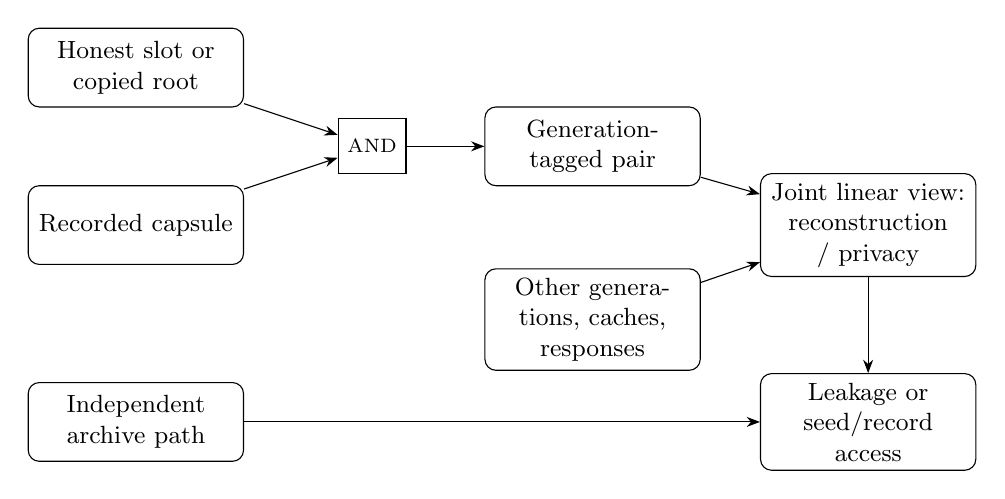
\begin{tikzpicture}[>=Stealth,box/.style={draw,rounded corners,align=center,font=\small,text width=25mm,minimum height=10mm},gate/.style={draw,rectangle,align=center,font=\scriptsize,minimum size=7mm}]
\node[box] (root) at (0,4.5) {Honest slot or copied root};
\node[box] (cap) at (0,2.5) {Recorded capsule};
\node[gate] (and) at (3,3.5) {AND};
\node[box] (pair) at (5.8,3.5) {Generation-tagged pair};
\node[box] (obs) at (5.8,1.3) {Other generations, caches, responses};
\node[box] (linear) at (9.3,2.5) {Joint linear view: reconstruction / privacy};
\node[box] (archive) at (0,0) {Independent archive path};
\node[box] (seed) at (9.3,0) {Leakage or seed/record access};
\draw[->] (root)--(and);\draw[->] (cap)--(and);\draw[->] (and)--(pair);
\draw[->] (pair)--(linear);\draw[->] (obs)--(linear);\draw[->] (linear)--(seed);
\draw[->] (archive)--(seed);
\end{tikzpicture}}
\caption{A capability hypergraph, not ordinary edge reachability. Conjunctive openings feed a joint observation module. An immutable copied root preserves its derivation despite honest deletion. Archive paths may bypass the ordinary sharing module. The module's reconstruction and privacy predicates are distinct.}\label{fig:capabilities}
\end{figure}

\subsection{Reconstruction and privacy are different predicates}
Let $S\in\mathcal D_1\times\cdots\times\mathcal D_k$ contain protected seed parameters, with each domain containing at least two field elements. Repeated generations of the same seed use the same coordinate. Let $R$ be an independent uniform vector of sharing/blinding coefficients over $\F_p$. For a fixed public operation choice, the accessible linear view is
\begin{equation}\label{eq:view}
 Y=A S+B R.
\end{equation}
All observation sources and public affine observations must be included. For privacy of a target subset conditioned on other seeds, their values are supplied to closure and their known contribution is subtracted; unknown nonuniform seeds are not silently treated as uniform masks.

\Needspace{12\baselineskip}
\begin{theorem}[Linear reconstruction and value-independent privacy]\label{thm:rank}
For the declared linear layer: (i) a seed coordinate is linearly reconstructible exactly when its unit row is in the row span of $[A\ B]$; (ii) the distribution of $Y$ is independent of all protected seed values exactly when
\begin{equation}\label{eq:privacy}
 \operatorname{rank}[B\ A]=\operatorname{rank}B.
\end{equation}
The privacy claim applies to arbitrary embedded seed domains as above. The reconstruction claim concerns linear decoders; with arbitrary bounded seed encodings, absence of its row-span witness does not rule out every nonlinear decoder.
\end{theorem}
\begin{proof}
A row-span representation gives a linear combination returning the selected coordinate; a linear decoder valid on all field inputs must have that coefficient row. For privacy, uniform $R$ makes $Y$ uniform on the coset $A s+\operatorname{im}B$. All these distributions agree if every column of $A$ lies in $\operatorname{im}B$. Conversely, changing only one seed between two distinct allowed values gives a nonzero scalar multiple of that column. Equality of cosets forces the column into $\operatorname{im}B$. Column containment is equivalent to~\eqref{eq:privacy}.
\end{proof}

For example, $Y=S_0+S_1$ with no masks linearly reconstructs neither coordinate but leaks their relation, violating joint privacy. Embedded domains can make such leakage even stronger. A deletion analysis must therefore name its predicate: preventing full linear reconstruction is weaker than preserving a value-independent view.

\begin{corollary}[Adaptive observations]\label{cor:adaptive}
Suppose observation choices depend only on the visible prefix, public seed-independent data, and fixed adversary coins. For each terminal transcript passing~\eqref{eq:privacy}, its probability mass is identical for every allowed seed vector. This is a statement about the accepted subdistribution, not conditioning on a potentially challenge-dependent freshness event.
\end{corollary}
\begin{proof}
Fix a terminal transcript and seed difference $\Delta$. The rank condition provides $d$ with $Bd=-A\Delta$. Translating the original uniform mask tape by $d$ while changing $S$ by $\Delta$ preserves every recorded answer. It therefore preserves every adaptive row choice and the entire transcript. Translation bijects the transcript fibers and preserves their probability mass. Public metadata or nonlinear observations omitted from~\eqref{eq:view} are outside the premise.
\end{proof}

\subsection{Erasure as witness elimination}
Fix public recorded facts $P$, immutable adversary copies $A_0$, and honest-origin facts $H$ eligible for the stated future snapshot. A permitted deletion $D\subseteq H$ leaves view roots $P\cup A_0\cup(H\setminus D)$. For either selected bad predicate $F$---declared reconstruction or failure of~\eqref{eq:privacy} after closure---let $\mathcal W_F$ be the inclusion-minimal supports $W\subseteq A_0\cup H$ for which $F(P\cup W)=1$.

\begin{theorem}[Witness-hitting characterization]\label{thm:cuts}
A permitted deletion prevents the selected bad predicate if and only if it intersects every support in $\mathcal W_F$. If a witness has no permitted honest-origin element, no allowed deletion can establish the selected property.
\end{theorem}
\begin{proof}
Both predicates are monotone under additional knowledge. A surviving unhit witness certifies failure. Conversely, if failure survives deletion, finiteness permits removal of redundant roots until a minimal surviving witness remains; it was not hit. An immutable witness cannot be hit by any permitted deletion.
\end{proof}

Thus a minimum-weight deletion can be formulated as a hitting-set optimization over witness supports. This is a standard monotone-access-structure formulation, not a new ordinary graph min-cut theorem. Threshold reconstruction and conjunctive decryption prevent replacement by simple edge reachability. Our exact implementation enumerates supports and deletions; no polynomial optimization guarantee is claimed. Privacy witnesses, rather than reconstruction witnesses, are required for a privacy promise: in the sum example, removing no facts already prevents linear recovery of $S_0$, but removing the sum observation is necessary for joint privacy.

\subsection{Independent generations and copied delivery credentials}
For epoch $e$, generation $g$ uses threshold $t_g$, distinct nonzero indices, and independently sampled polynomials
\begin{equation}\label{eq:sharing}
 A_g(X)=S_e+\sum_{i=1}^{t_g-1}a_{g,i}X^i,
 \qquad B_g(X)=\sum_{i=0}^{t_g-1}b_{g,i}X^i.
\end{equation}
Pedersen coefficient commitments are $g_0^{a_{g,i}}h_0^{b_{g,i}}$, with $a_{g,0}=S_e$. Their exponent representation, using $h_0=g_0^\beta$, is a stronger affine view; hiding that view suffices to hide the actual commitments. Let $I_g$ include every genuine share/opening pair obtainable across the full recorded history by that generation's capabilities, not only currently held shares.

\begin{theorem}[Joint independent-generation characterization]\label{thm:temporal}
Assume honest generation, mutually independent polynomial randomness, no extra coefficient/seed observations, and the declared capsule-opening interfaces. The joint commitment/opening view of any finite collection of generations of $S_e$ is independent of $S_e$ if and only if $|I_g|<t_g$ for every generation. This also holds on adaptive terminal transcripts satisfying those conditions.
\end{theorem}
\begin{proof}
For each subthreshold terminal set, the polynomial translation in Appendix~\ref{app:proofs} changes the common constant by the same $\Delta$ while preserving all that generation's commitments/openings. Independent random-coefficient blocks permit simultaneous bijective translations, preserving the joint adaptive transcript. If one generation exposes at least $t_g$ distinct pairs, interpolation returns $S_e$, so privacy fails.
\end{proof}

The rule layer determines $I_g$. Reused recipient keys may open old and future capsules; a captured bank can include future period slots even when the periods' keys were originally independent. Renewing recipient banks removes old-key rules to \emph{new} capsules but cannot remove prior observations. Refreshing an already known $S_e$ cannot restore its secrecy. Conversely, a fresh independent epoch seed can pass the target privacy test even conditioned on all old seeds when its renewed delivery paths and auxiliary disclosures leave the new view subthreshold.

Independence is essential. Reusing polynomial randomness across generations can produce a joint rank failure while every individual generation has fewer than $t_g$ disclosed points. Auxiliary coefficient leaks, correlated sharings, alternate authorities and changed thresholds must be analyzed with the general closure/rank condition, not the per-generation counting shortcut. These statements are not an active distributed proactive-sharing protocol.

\subsection{The single-generation deletion bound as a specialization}
With one generation and one useful point per index, suppose $q_d$ matching receipts include at most $f$ dishonest issuers, honest signers remove every local path, and $c$ otherwise-erased honest indices have useful prior copies. At least $\max(0,q_d-f)$ indices lose their honest paths; remaining indices plus prior copies give the tight worst-case bound
\begin{equation}\label{eq:deletion}
 m_{\max}=\min(n,n-q_d+f+c),\qquad
 q_d\ge n-t+f+c+1\ \Longleftrightarrow\ m_{\max}<t.
\end{equation}
Tightness places as many liars as possible among signers and copies at distinct honest erasers. The temporal theorem then supplies sharing-view privacy. This recovers the existing elementary result, but only for the stated single-generation/path assumptions. A signed receipt does not prove their physical truth.


\section{Reference protocol, assumptions and component security}\label{sec:protocol}

\subsection{Explicit exposure interfaces}
Table~\ref{tab:oracles} specifies the trace-level observations used by the analysis. An honest party's state and the challenger's private bookkeeping are distinct. The exposure inventory must enumerate storage wrappers, snapshots and volatile work; deletion of one named field is not proof that this inventory is exhaustive.

\begin{table}[htbp]
\caption{Trace interfaces and returned material. A real device disclosure may cross several compromise categories when keys are co-resident.}\label{tab:oracles}
\centering\footnotesize
\begin{tabularx}{\linewidth}{@{}p{.26\linewidth}Y@{}}\toprule
Interface & State or observation supplied\\\midrule
Setup / Publish & Honest bank directories, epoch/generation parameters, public manifests, commitments and recorded capsules\\
CopySlot$(h,b,e)$ & The present matching private slot, or failure if absent; an earlier copy remains in adversary state\\
CopyBankCapability & Every retained slot in that bank snapshot, including future periods; no signing authority is implied by this narrower interface\\
CorruptDevice & Enumerated stored slots, cached shares, wrapper roots and volatile responses; stored signing keys, if present, also count as identity compromise\\
CorruptIdentity & Specified signing/policy keys and malicious voting control, without inventing possession of a data slot\\
CopyPair / CopyResponse & The declared pair or recorded response-opening material; irreversible deliveries are never retracted\\
CorruptRecoverer & Its reconstructed seeds, available pairs, plaintext outputs, ephemeral session state and buffers\\
CorruptArchive & The specified independent archival root/slots and their recorded envelopes\\
Expire / Crash / Restart & Lifecycle transitions; receipts and public log metadata only. Old snapshots must pass the nonrollback anchor\\
FinalSnapshot & Exactly the honest-origin fields allowed by the experiment's exposure map, followed by declared closure\\\bottomrule
\end{tabularx}
\end{table}

The ideal seed-view game lets an adversary nominate two allowed seed vectors with identical public metadata, samples a hidden bit and uniform sharing masks, and answers adaptive declared observations. Recorded encryption envelopes are opaque symbols in this game. At the final observation it applies the rank-privacy freshness test; on accepted runs it outputs whether the guess equals the bit, and otherwise an independent fair bit. The advantage is always
\begin{equation}\label{eq:advantage}
 \Adv_{\mathrm{view}}(\mathcal A)=\left|\Pr[\mathsf{out}=1]-\tfrac12\right|.
\end{equation}
Corollary~\ref{cor:adaptive} gives zero advantage for the accepted linear-view subdistribution. This is a complete statement about that ideal experiment. It does not include concrete ciphertext leakage or arbitrary computations on restored challenge plaintext. A concrete historical-data game would require a separate refinement/composition theorem; this paper does not claim one. The earlier schematic protocol-level bound is therefore not retained as a theorem.

\subsection{A concrete classical profile}\label{sec:profile}
The selected profile uses independent 32-byte epoch seeds embedded in the scalar field of NIST P-384. The sharing prime is the group order, not the curve-coordinate prime (hexadecimal; concatenate the three lines):
\begin{Verbatim}[fontsize=\small]
FFFFFFFFFFFFFFFFFFFFFFFFFFFFFFFF
FFFFFFFFFFFFFFFFC7634D81F4372DDF
581A0DB248B0A77AECEC196ACCC52973
\end{Verbatim}
Scalars use 48-byte unsigned big-endian encodings strictly below that prime. Coefficients and blinders are uniform including zero. Holder indices are distinct nonzero elements, with profile limit $n\le255$. P-384 commitments use the standard generator and a second generator obtained with RFC~9380 suite \code{P384\_XMD:SHA-384\_SSWU\_RO\_}, message \code{h}, and domain tag \code{CEAB-v2-Pedersen-H}, retrying with an encoded counter for identity or $\pm g_0$~\cite{rfc9380,sec2}. The unknown generator relation is an assumption of this instantiation; it is not established by the toy algebra checker. Compressed commitment points occupy 49 bytes.

\begin{table}[htbp]
\caption{Concrete algorithm choices. Specifying the profile is separate from implementing or proving its complete composition.}\label{tab:profile}
\centering\footnotesize
\begin{tabularx}{\linewidth}{@{}p{.24\linewidth}Y@{}}\toprule
Component & Profile and binding requirements\\\midrule
Capsule PKE & RFC~9180 HPKE Base; DHKEM(X25519, HKDF-SHA256), KEM 0x0020; KDF 0x0001; ChaCha20Poly1305 AEAD 0x0003. Independent finite-bank slots; signed manifest supplies sender/context authentication~\cite{rfc9180}\\
Object PRF & HMAC-SHA256 under the uniform 32-byte epoch seed, over typed deterministic CBOR containing domain, account, creation configuration, birth epoch, object ID and immutable header\\
Data AEAD & ChaCha20-Poly1305; nonce is four zero bytes followed by the uint64 big-endian chunk index, never repeated under an object key. Profile limit $2^{32}-1$ chunks, at most 1 MiB each~\cite{rfc8439}\\
Signatures & Pure Ed25519 on SHA256 of a typed, domain-separated complete-message encoding; canonical validating verification. This is not Ed25519ph~\cite{rfc8032}\\
Hash and encoding & SHA-256; RFC~8949 core deterministic CBOR, definite lengths and bytewise encoded-key ordering. Reject duplicates, unsupported required fields, invalid scalars/points and oversized requests~\cite{rfc8949}\\
Private release & Short-lived authenticated TLS~1.3 with forward-secret ephemeral exchange, exporter binding to the approved recipient/request, no release in early data, and explicit session/buffer cleanup~\cite{rfc8446}\\\bottomrule
\end{tabularx}
\end{table}

Capsules contain exactly a share and blinder, 96 raw bytes. HPKE info binds account, configuration, bank, epoch, generation and holder; associated data additionally binds commitments, package identity and algorithms. The data header is immutable and authenticated. Random 32-byte object identifiers give collision probability at most $q(q-1)/2^{257}$ for $q$ independently sampled IDs. An uncertain interrupted creation is abandoned under a fresh identifier rather than reusing a key/nonce for changed plaintext. The overall profile targets approximately 128-bit classical strength, bounded by its weakest components; a 256-bit seed is not a blanket 256-bit security claim.

\subsection{Exact slot-component game and guessing losses}\label{sec:slots}
The slot game creates $nT$ independent labeled PKE pairs. It exposes every public key and permits recording all capsules before or after deletion. One challenge encrypts the adversary's equal-length pair under a selected guardian/period key. Other slots can be exposed completely. Labeled decryption queries are permitted except for the exact protected challenge. Freshness excludes every earlier target-slot disclosure, including a regenerating wrapper, secondary store or rollback image. A later snapshot contains only genuinely retained slots. Nonfresh outcomes use the fair-bit convention in~\eqref{eq:advantage}.

\begin{lemma}[Independent-slot component]\label{lem:slot}
Under the specified labeled IND-CCA PKE interface and actual target-slot erasure, a selective guardian/period challenge reduces to one PKE challenge without a slot-guessing factor. Selecting only the period adaptively among $T$ incurs at most $T$; selecting only the guardian among $n$ incurs at most $n$; selecting both among $nT$ incurs at most $nT$, with polynomial setup/query work.
\end{lemma}
\begin{proof}
Embed the PKE challenge public key at the selected or guessed pair and generate all other keys. The public directory has the honest independent distribution. Other-slot disclosures are answerable; target decryption queries go to the CCA oracle except the prohibited challenge. A fresh post-deletion snapshot never needs the unknown target secret. Premature target exposure or a wrong target guess yields an independent fair outcome. Uniformly guessing the unfixed coordinates supplies the stated factors.
\end{proof}

For a fixed target epoch, masking at most $n$ recipient capsules is a separate $n$-hop argument using selective-pair component challenges. If an outer experiment guesses one of $N$ epochs, its corresponding accounting is $Nn$, not $NnT$ when $N$ already enumerates the challenged periods. A guessed final useful-index set would introduce a separate partition loss; no such completed concrete-data reduction is asserted here. Independent data entropy alone cannot heal a stolen bank containing enough future slots.

\subsection{Operational assumptions and failure terms}
\begin{table}[htbp]
\caption{Assumptions, dependent statements and failure consequences.}\label{tab:assumptions}
\centering\footnotesize
\begin{tabularx}{\linewidth}{@{}p{.26\linewidth}YY@{}}\toprule
Assumption & Dependent result & If absent\\\midrule
Complete declared inventory and affine-view coverage & Closure/privacy application & An omitted wrapper or nonlinear client observation invalidates the application\\
Honest independently randomized sharing & Temporal specialization & Malicious/correlated generation requires another analysis\\
Actual honest cleanup, including wrappers and buffers & Post-barrier bound & A retained or resurrected path remains useful\\
Independent recipient slots & Slot component & Other-key exposure can recreate a target key\\
Authentic ordered log/checkpoints & Release ordering and policy & Replay, rollback or conflicting accepted states\\
External authentic bootstrap & Identity recovery & Cloned/replaced authority can persist\\
Private bound release and cleanup & Observation inventory & Recorded responses may add useful pairs\\
Persistent monotone clock & Mandatory hold/deadline & Premature release or unbounded waiting\\
Stated total prior-copy budgets & Counting specialization & More historical indices survive than counted\\\bottomrule
\end{tabularx}
\end{table}

Failure probabilities are not hidden inside a generic negligible implementation term. For an explicitly chosen finite experiment, define the global union budget
\begin{align}\label{eq:budget}
 B_{\mathrm{all}}={}&\delta_{\mathrm{log}}+\delta_{\mathrm{erase}}+\delta_{\mathrm{chan}}
 +\delta_{\mathrm{clock}}+\delta_{\mathrm{boot}}\\
 &+K_{\mathrm{sig}}\varepsilon_{\mathrm{sig}}+\varepsilon_H+\varepsilon_{\mathrm{DL}}.\nonumber
\end{align}
Under the relevant component reductions this upper-bounds the union of the named failure events; it is not a completed bound on historical ciphertext advantage. Every $\delta$ is global over all relevant operations. Without physical/platform or behavioral models, these terms have no measured or asserted negligible value.

\begin{table}[htbp]
\caption{Interpretation of the failure budget. Query/resource bounds are part of every primitive term.}\label{tab:budget}
\centering\footnotesize
\begin{tabularx}{\linewidth}{@{}p{.20\linewidth}YY@{}}\toprule
Term & Event measured & Required contract/evidence\\\midrule
$\delta_{\mathrm{log}}$ & Any relevant freshness/finality/durability failure & Chosen log's locking, restart and reconfiguration assumptions\\
$\delta_{\mathrm{erase}}$ & Any relevant honest cleanup/anti-rollback failure & Complete logical and physical path model; excludes attacker copies already charged to exposure\\
$\delta_{\mathrm{chan}}$ & Any private endpoint/session binding or cleanup failure & Actual release transport and recorded-session exposure semantics\\
$\delta_{\mathrm{clock}}$ & Any monotone/rate-bound failure & Trusted timing persistence through restart\\
$\delta_{\mathrm{boot}}$ & Any bootstrap/authority-anchor failure & Independent authentic recovery enrollment/anchor\\
$K_{\mathrm{sig}}\varepsilon_{\mathrm{sig}}$ & Forgery under any honest identity & Per-key EUF-CMA bound with experiment signing-query limits; union over keys\\
$\varepsilon_H$ & Any relevant context/manifest hash collision & Global collision bound for the exact typed encodings and query limits\\
$\varepsilon_{\mathrm{DL}}$ & First accepted distinct false opening & One DL extraction algorithm with all $V$ verification attempts in its resource bound; no extra $V$ factor is silently assumed\\\bottomrule
\end{tabularx}
\end{table}

The false-opening extraction is elementary: a reference pair $(a,b)$ and distinct accepted $(a',b')$ satisfy $a+\beta b=a'+\beta b'$. Distinctness implies $b\ne b'$, yielding $\beta=(a-a')/(b'-b)$. This requires an honest reference sharing and validated group encodings, not malicious-dealer agreement.

\section{Joint progress and lifecycle guarantees}\label{sec:lifecycle}

\subsection{Quorum feasibility and human approval}
Let $u$ additional honest holders be unavailable. Share reconstruction and deletion progress require $t,q_d\le n-f-u$. Combining with~\eqref{eq:deletion} yields
\begin{equation}\label{eq:feasible}
 t\ge2f+c+u+1,\qquad n\ge3f+c+2u+1.
\end{equation}
Conversely these arithmetic requirements admit $t=2f+c+u+1$ and $q_d=n-f-u$ when the last inequality holds. Approval progress separately needs $q_a\le n-f-u$. Requiring at least $k$ honest signatures in any approval certificate needs $q_a\ge f+k$. Log-quorum intersection and progress require
\begin{equation}\label{eq:log}
 2q_l>n+f,\qquad q_l\le n-f-u,
\end{equation}
which admits a quorum only if $n\ge3f+2u+1$. These are service-level parameter conditions, not a construction of Byzantine consensus.

At most $f$ identities can account for Byzantine signatures in a $q_a$-signer malicious certificate. The rest, at least $q_a-f$, are genuine honest false approvals. Let $\alpha$ be the probability of that joint event over all repeated interactions and malicious policy-changing requests. Then unauthorized honest release is bounded by $\alpha$ plus the relevant control-failure events. Neither independence nor a numeric value for $\alpha$ is assumed; it can be one. The guarantee binds a quorum to a request and mandatory delay, not to correct human recognition.

\begin{table}[htbp]
\caption{Feasibility sensitivity at the mathematical minimum. These are not deployment recommendations. The displayed quorums all equal $n-f-u$ and satisfy~\eqref{eq:log}.}\label{tab:sensitivity}
\centering\small
\begin{tabular}{@{}rrrrrr@{}}\toprule
$f$&$c$&$u$&Minimum $n$&$t$&$q_d=q_a=q_l$\\\midrule
0&0&0&1&1&1\\
1&0&0&4&3&3\\
1&1&0&5&4&4\\
1&1&1&7&5&5\\
2&1&1&10&7&7\\
2&2&2&13&9&9\\\bottomrule
\end{tabular}
\end{table}

\subsection{Generation-aware state machine}
Each path $(e,g)$ moves through sealed, expiring and erased states. Requests move through holding, decrypting, queued, sending and terminal states. Decryption completion and irreversible transfer are separate transitions; a pre-expiry check does not authorize a later unchecked send. The only disclosure event is the first irreversible byte transfer, conservatively charged as a complete pair even when the send is interrupted. An already delivered pair remains an adversarial capability after expiry.

Expiry atomically persists its tombstone and cancels owned work/buffers for that path. Slot deletion precedes an honest receipt. A proposed log barrier is not a committed barrier. The effective record floor advances only after every modeled generation at that birth epoch commits its barrier and all prior birth epochs have done so. Configuration activation cancels old work; a proposed configuration does not activate on crash recovery. Restart uses current durable metadata, and an old image cannot override the assumed nonrollback anchor.

The five safety properties are: no irreversible release after expiry; exact request/recipient binding; monotone effective floor; honest receipt only after cleanup; and no queued stale work for expiring or obsolete configuration paths. Initialization and each transition preserve these properties under the stated abstract services; Appendix~\ref{app:lifecycle} gives the inductive cases. This argument is manual, while the finite checks below use TLC. Neither establishes a cryptographic implementation or an unconditionally available log.

\subsection{A specified conditional recovery deadline}
For a conservative serial schedule, obtain a nonce-bound checkpoint in one round $D$, fetch complete packages in one $D$, commit/disseminate the request in one log service call $C$, wait for both approvals and local holds, commit/disseminate the approval certificate in one $C$, establish a bound ephemeral channel in one $D$, and obtain share responses in one $D$, followed by local work $P$. Here $C$ includes submission transport, finality and delivery to the participating honest parties. Let $H$ bound availability of the required real approvals after request observation.

With clock rates in $[1-\rho,1+\rho]$, $0\le\rho<1$, waiting $(1+\rho)\tau$ local units lasts at least $\tau$ and at most $(1+\rho)\tau/(1-\rho)$ real units. For this chosen schedule,
\begin{equation}\label{eq:deadline}
 T_{\mathrm{restore}}\le4D+2C+
 \max\!\left\{H,\frac{1+\rho}{1-\rho}\tau\right\}+P.
\end{equation}
All targets must retain at least this slack, and enough holders, storage and authentic bootstrap must survive. The constants count specified stages; $D,C,H,P$ are assumptions, not measured system latencies. Permanent suppression or expiry during the hold yields failure, never timeout-created approval.


\section{Verification and reproducible evidence}\label{sec:evaluation}

\subsection{Retained baseline and independent algebra checks}
We preserve the baseline programs and all five original regression tests. Their reproduced JSON outputs are compared for complete equality with the saved baseline outputs. The deletion enumeration retains 14,714 adversary cases and 2,150 threshold configurations over $1\le n\le8$ and bounded liar/copy sets. The original toy sharing check retains 15,625 assignments over $\F_5$; static authorization retains 320 approver/time cases, seven field mutations and expiry rejection; symbolic retention retains 39 cases. The original expanded exploration retains 288 quotient states and 732 edges over three separate one-generation configurations, together with 121 independent two-generation rank patterns. These checks remain arithmetic/symbolic evidence, not measured attack probabilities.

The new algebra checker compares the rank-privacy prediction with direct output-distribution enumeration and the reconstruction prediction with direct all-input fiber enumeration. It checks 7,407 matrices over $\F_3$ spanning several one/two-seed, one/two-mask and one/two-output dimensions. Thus the reference check is not another invocation of the same Gaussian-elimination decision. It also checks 256 independent-generation exposure-pattern pairs over $\F_7$ with thresholds two or three, and a correlated-randomness counterexample. An independent enumeration of actual share/deletion pairs and approval/log quorums checks 28,335 parameter configurations with $n\le20$; exactly 1,914 meet all joint constraints, agreeing with~\eqref{eq:feasible}.

For the cut characterization, a two-of-three ordinary path plus an archive has four minimal reconstruction supports: the three ordinary pairs and the archive root. The minimum deletion has size three when all four roots are deletable: two ordinary roots and the archive root. If the archive root is immutable, allowed erasure is impossible. Twenty-eight deletion/copy combinations agree with the witness-hitting characterization. A relation-only fixture independently distinguishes a privacy cut from a reconstruction cut.

\subsection{Temporal exploration and shortest witnesses}\label{sec:temporal-evidence}
The new breadth-first explorer uses labeled publish/refresh/disclosure actions and the full closure/rank decision. It retains old capsules and observations, distinguishes renewed bank labels, permits client/archive disclosures, and varies thresholds. Each atomic bank-copy action ends before the next visit, so traces can accumulate data capabilities without simultaneous control of several devices; this is not an assertion that their signing identities remain uncompromised under arbitrary physical device capture.

The eight runs contain 120 states and 174 transitions in total. These are separate bounded scenarios, not one combined global state graph. Two scenarios preserve target privacy under their stated exposures; six have a saved shortest privacy counterexample. The exact traces and accessible observation sets are included in the artifact.

\begin{table}[htbp]
\caption{Temporal scenarios. ``Private'' refers to the declared target view, conditioned on other seed values. Each run uses three holders and at most two generations/epochs.}\label{tab:temporal}
\centering\footnotesize
\begin{tabularx}{\linewidth}{@{}p{.43\linewidth}rrY@{}}\toprule
Scenario & States & Private? & Distinguishing outcome\\\midrule
Independent share refresh &21&Yes&One copied pair per generation remains jointly hidden\\
Correlated refresh randomness &21&No&Different-index subthreshold pairs combine across reused randomness\\
Fresh seed, stolen future bank &21&No&Old bank snapshots open fresh-epoch capsules\\
Renewed recipient bank &21&Yes&Old copies open no new-bank capsule, even with old seed known\\
Threshold lowered, recipients reused &21&No&Two old recipient capabilities cross the new threshold\\
Known seed then independent refresh &5&No&Recipient renewal cannot revoke the reconstructed seed\\
Recovery-client exposure &4&No&The reconstructed target seed is directly disclosed\\
Archive after ordinary erasure &6&No&An independent archive still supplies the historical seed\\\bottomrule
\end{tabularx}
\end{table}

For example, the future-bank witness publishes the old epoch, copies two old-bank holder capabilities, then publishes the fresh independent epoch under that bank. The new seed is exposed through future slots. In the threshold-change witness, two capabilities remain below the old threshold three but become sufficient after a threshold-two generation uses the same delivery bank. In the correlated-randomness witness, two generations each disclose one pair at different indices; the shared coefficient block permits reconstruction. Each violates an enlarged interpretation, not Theorem~\ref{thm:temporal}'s independence and complete-history premises.

The archive witness completes the assumed ordinary-path deletion while retaining an archive envelope and subsequently discloses its archive key. This demonstrates why an ordinary-only compromise promise is different from revoking all recovery routes. The explorer assumes the named ordinary cleanup event; its physical implementation is not verified by this trace.

\subsection{TLA+ lifecycle checks and mutation controls}\label{sec:tlc}
The TLA+ specification represents one honest guardian's path obligations, two classes of certificate (exact or mismatched), recipient mutation, delayed hold completion, configuration activation, a separate identity-compromise step, crash/restart, and attempted rollback. Signature/log validity is abstract. Offering an exact certificate does not assume human intent is correct; the environment may produce genuine false approvals. Identity compromise does not automatically reveal a data slot. These abstractions deliberately separate trace binding from authentication cryptography.

TLC2~2.19 from release 1.7.4 is pinned by SHA-256 and executed with one breadth-first worker, seed 1 and fingerprint polynomial index 0. Table~\ref{tab:tlc} reports the reachable states. The total 316,332 is the sum of four separate safe model runs. The epoch/generation variables are explicit, and the floor counts completed birth epochs only after all their generation barriers. Deadlock/liveness checking is disabled; withholding and cancellation are allowed. Finite safety checking does not imply an unconditional recovery-time guarantee~\cite{lamport2002}.

\begin{table}[htbp]
\caption{Final TLC safe configurations. Every listed state satisfies all five lifecycle invariants and the type invariant.}\label{tab:tlc}
\centering\small
\begin{tabular}{@{}lrrrr@{}}\toprule
Configuration & Epochs & Generations & Requests & Distinct states\\\midrule
SafeOneEpoch&1&1&2&26,448\\
SafeTwoEpoch&2&1&1&5,444\\
SafeCombined&2&1&2&132,232\\
SafeGenerations&1&2&2&152,208\\\bottomrule
\end{tabular}
\end{table}

Four deliberate unsafe variants ensure the checks reject the intended failures. Without queue cancellation and final rechecks, TLC finds request, hold, exact certificate, decryption, queue/send preparation, expiry, and then transfer. Without the receipt guard, expiry followed immediately by receipt signing violates cleanup ordering. Without rollback protection, expiry, deletion, receipt, proposal, commit, crash and old-image restart decrease the floor and resurrect a path. Without binding validation, a mismatched offered certificate permits transfer. The raw breadth-first logs provide shortest-action counterexamples for each selected invariant. A specification error in Boolean flag assignment was found by these negative controls and corrected before accepting the final runs.

TLC's state fingerprints have the collision estimates reported in the raw logs. The finite results corroborate the action-level inductive argument; neither is a TLAPS proof or a refinement proof of a deployed client, consensus implementation or physical storage platform.

\subsection{Executable critical-path reference}
The reference kernel implements generation-tagged durable state, request binding, distinct signer counting, a restricted core-deterministic CBOR encoder, held decryption work, queued buffers, atomic modeled first-byte ownership transfer, expiry cancellation, and crash/restart with an assumed nonrollback anchor. Decryption is split into begin/finish calls so a scheduled real thread can pause while another thread expires the path. The resumed completion is rejected rather than reintroducing a stale response.

Twenty-five new tests exercise the report's named cases: expiry before release, during decryption, after decryption and before transfer; an interrupted send after disclosure; crashes after expiry intent, slot removal, receipt and pending/committed barriers; old snapshots; incomplete configuration commits; replay, recipient/field mutation and duplicate identities; stale checkpoints; refusal to supply a quorum; genuine false approval; clock rollback; and interactions between two generations before advancing an epoch floor. All pass alongside the five preserved tests.

This kernel does not implement PKE, real signatures, network TLS or Byzantine consensus. A buffer-overwrite test concerns logical application state, not physical destruction of every Python or operating-system copy. Its trusted-verifier certificate objects are not cryptographic signatures. We report no setup/recovery/expiry benchmark, hardware deletion certification or human-risk estimate. A full cryptographic prototype is optional for this formal-analysis track and is not substituted with invented measurements.

\subsection{Artifact access and reproduction}\label{sec:artifact}
The versioned artifact includes source, saved and reproduced outputs, shortest traces, configs, the pinned TLC digest, Python/Java versions, expected results, tests and a SHA-256 manifest. Version 2.0.0 is available at \url{https://github.com/SamarjeetMalik/threshold-backup-capability-accounting/releases/tag/v2.0.0}. Run the supplied Python reproduction entry point for baseline/algebra/temporal/kernel checks; invoke the TLC runner with Java 17 and the pinned jar for all safe and unsafe configurations. The exact commands and dependency-fetch checksum are in the artifact README. The manuscript and artifact identify their version together; no DOI is claimed.

\section{Costs, boundaries and unresolved obligations}\label{sec:limits}

\subsection{Analytical costs and implementation evidence}
A finite $T$-slot X25519 bank stores $32T$ raw secret bytes per guardian, or 11,680 bytes for $T=365$, before metadata/protection. With 48-byte scalar pairs, a capsule has 96 raw payload bytes; a 32-byte encapsulated key plus 16-byte tag gives approximately 144 bytes, or 720 bytes for five, before context and signatures. Four compressed P-384 commitments add 196 bytes. These are encoding calculations. Bank setup is $O(nT)$, naive sharing $O(nt)$ field work and interpolation $O(t^2)$; closure is polynomial in the finite declared graph and matrix sizes, while exact minimal-witness/deletion enumeration can be exponential.

Implementation evidence consists of the executable lifecycle behavior and scheduled tests, not measured cryptographic throughput, network cost or deployment reliability. Comparisons with a real CKS/GKP/ephemerizer implementation would need matched access, retention and trust assumptions. Additional performance data would be a separate systems contribution rather than evidence for the rank theorem.

\subsection{Four limitation categories}
\paragraph{Cryptographic.}
The general theorem concerns declared symbolic operations and affine observations. Row-span non-reconstruction is not arbitrary computational secrecy, and ciphertext composition is not proved by symbolic closure. The concrete profile's primitive assumptions, generator selection and application nonce discipline require independent implementation validation. No scalable adaptive end-to-end backup theorem, active proactive-sharing protocol or retrospective revocation is established.

\paragraph{Distributed systems.}
The log, exact certificates, nonrollback anchor and timing services are explicit contracts. TLC proves finite trace safety under those abstractions, not quorum-service implementation or unconditional liveness. The reference transfer is an atomic modeled handoff; mapping an actual buffered transport and crash persistence to it needs a separate refinement proof. Configuration/identity recovery cannot be authenticated solely by already cloned authority.

\paragraph{Operational erasure.}
An inventory can omit disk roots, swap, dumps, snapshots or external copies. Honest receipts do not certify that none exist. Already delivered responses and reconstructed seeds remain useful forever in the adversarial view. An ordinary erasure promise must say whether archives and alternate authorities are excluded or also removed.

\paragraph{Human and institutional trust.}
Distinct labels are not independent administrative domains. Real approval signatures may embody a mistaken ceremony, with $\alpha$ unconstrained by this analysis. Authenticated bootstrap, custody enrollment and institutional independence need separate evidence. Nothing here estimates phishing success or guarantees recovery after all factors are lost.

\section{Conclusion}
Capability exposure accounting requires both an inventory of derivation paths and a definition of what it means for the surviving view to be safe. The declared closure characterizes symbolic/linear reconstruction; the rank condition gives the stronger value-independent privacy test for affine observations. Minimal witness supports characterize which permitted deletions suffice, while copied roots and independent archives can make such deletion impossible. The temporal specialization explains the different roles of sharing refresh, credential renewal and fresh record seeds. Quorum feasibility and checked lifecycle order make the operational assumptions visible. The contribution is this explicit, executable analysis and its scoped proofs; a complete concrete-client cryptographic refinement and physical-erasure realization remain unresolved.


\backmatter
\bmhead{Declarations}
This manuscript reports formal analysis, finite model checks and a reference implementation. It reports no study involving human participants or personal data. The artifact's version and access location appear in Section~\ref{sec:artifact}. The affiliations shown are author supplied.

\begin{appendices}
\section{Polynomial translation and component details}\label{app:proofs}

\subsection{Joint hiding with Pedersen verification material}
Fix a generation of threshold $t$ and a terminal set $I$ of $k<t$ distinct nonzero disclosed indices. Let
\[
 Q(X)=\prod_{x\in I}(X-x),\qquad
 D(X)=\Delta Q(X)/Q(0).
\]
For $I=\varnothing$ the empty product is one. Since $Q(0)\ne0$, $D(0)=\Delta$, $D(x)=0$ at every disclosed index, and $\deg D<t$. Write $h_0=g_0^\beta$ for fixed nonzero $\beta$. Translate the polynomials by
\[
 A'(X)=A(X)+D(X),\qquad B'(X)=B(X)-D(X)/\beta.
\]
This changes the constant of $A$ from $s$ to $s+\Delta$. It preserves both coordinates $(A(x),B(x))$ at every $x\in I$. It also preserves every exponent $a_i+\beta b_i$, hence every coefficient commitment. For each allowed seed value, the nonconstant $a_i$ and all $b_i$ are independent uniform field elements. The translation bijects those coefficient spaces and preserves probability exactly. Its proof can use $\beta$ even though parties cannot compute it; this is an information-theoretic hiding argument, not a binding algorithm.

For several independent generations, perform that translation separately in each coefficient block with the same seed shift. The product map is a bijection preserving their entire joint view. An adaptive transcript fixes its terminal index sets; preserving all answers preserves the choice of each next query. If a generation exposes $t$ points, ordinary interpolation distinguishes any two distinct seeds. This proves both directions of Theorem~\ref{thm:temporal}, including $t=1$: only an empty disclosure set is then private. A correlated block need not admit the separate translations, which is exactly why its joint rank must instead be tested.

For fresh independent epochs, apply the translation only to the target epoch blocks, holding all older seed values and old-epoch observations fixed. This proves the stated conditional privacy when old credentials open no additional target observations. It does not apply if those credentials still decrypt target capsules or an archive directly exposes the target seed.

\subsection{Sharing, reconstruction and binding}
An honest writer samples~\eqref{eq:sharing}, publishes coefficient commitments $C_i=g_0^{a_i}h_0^{b_i}$, and encapsulates $(A(x_h),B(x_h))$ to each holder's authenticated epoch/bank slot. A recoverer rejects duplicate holder indices, validates encodings and the signed manifest, and checks
\[
 g_0^{A(x_h)}h_0^{B(x_h)}=\prod_{i=0}^{t-1}C_i^{x_h^i}.
\]
Any $t$ accepted genuine pairs reconstruct the seed using
\[
 S_e=\sum_{h\in I} A(x_h)
 \prod_{k\in I\setminus\{h\}}\frac{-x_k}{x_h-x_k}.
\]
The denominators are nonzero by distinctness. Verification alone does not establish an honest dealer or agreement on a commitment vector. The manifest/log contracts supply the selected vector. Given an honest reference opening, a distinct accepted opening yields the discrete-log extraction stated in Section~\ref{sec:protocol}. This is the particular binding use in the failure budget, not a malicious-dealer VSS theorem.

\subsection{Authoritative ideal-game convention}
The following defines the finite linear-view game independently of any production ciphertext experiment. Setup fixes a finite public inventory and operation language. The adversary supplies two seed vectors in the allowed Cartesian domain and matching public metadata. The challenger samples a fair bit, a uniform full mask tape, and answers the named trace interfaces; rules exposing observations return the relevant affine rows evaluated on that seed/mask tape. A recorded opaque envelope reveals its type and declared public metadata only. The adversary may adapt its next operation to the visible prefix. At termination, compute declared closure and the rank test for the selected target seeds conditioned on the other seeds. On a passing transcript return the correctness bit; on a failing transcript return a fresh fair bit.

The passing transcript masses agree branch by branch by Corollary~\ref{cor:adaptive}, so the output probability is exactly one half. Direct target-seed or restored-plaintext disclosures cannot be hidden by labeling a recovery opaque; they are observations outside the protected view and invalidate that application. This ideal experiment proves neither IND-CCA security of the selected HPKE composition nor security of a client which computes arbitrary functions of restored plaintext. The component-security choice in this paper deliberately leaves that composition theorem open.

\section{Lifecycle induction and operational schema}\label{app:lifecycle}

\subsection{State and invariants}
The released \code{RecoveryLifecycle.tla} uses paths $(e,g)$, a finite request set, persistent expiry tombstones, slot-presence bits, receipts, proposed/committed barriers, and a configuration counter. Volatile request state separates holding, decrypting, queued, sending, done and cancelled. Only \code{Transfer} grants external knowledge. The effective floor is the number of consecutive birth epochs for which \emph{all} modeled generation barriers have committed.

In addition to the five safety properties, use these helper facts: receipts imply tombstones and absent slots; a committed barrier requires its receipt and the preceding-epoch barriers; buffers belong only to queued/sending jobs; tombstones grow; and activated configurations do not decrease. The floor is a prefix property rather than a promise that a later generation can be silently created below it. Enrollment of paths for a live epoch must be complete before its floor commitment; creating a fresh obligation below an already committed floor is forbidden by the protocol specification.

\subsection{Inductive transition cases}
Initialization has no work, receipts or barriers and therefore satisfies the invariants. \code{Request}, \code{OfferCertificate}, \code{HoldCompletes}, endpoint mutation and the separate identity-compromise environment action do not transfer data. Request identifiers cannot be reused. An offered token can be mismatched; offering it is not verification.

\code{BeginDecrypt} checks path liveness, exact request binding, current configuration and completed hold. \code{FinishDecrypt} and \code{StartSend} repeat the necessary checks. Thus expiry or a configuration change cannot turn stale decryption work into a valid new buffer. \code{BeginExpiry} persists the tombstone and invalidates all owned work and buffers for that path atomically. \code{Erase} removes the local slot. \code{SignReceipt} requires both the slot and owned buffers absent. A proposed barrier changes neither commitment nor floor. \code{Commit} requires its receipt and all preceding epoch paths committed, so adding a generation barrier cannot decrease the floor and cannot advance it prematurely.

\code{Transfer} is the only irreversible release. Its safe guard checks a live path, exact bound recipient/request, current configuration and hold completion. Hence it preserves both release flags. Once it happens, the model charges the entire pair to the adversary even if a network send later aborts. Expiry need only cancel still-owned work; it never retracts that disclosure.

Configuration activation cancels work before changing the active version. Crash drops volatile jobs and buffers while preserving tombstones, slot absence, receipts, proposals and committed metadata. Restart preserves durable state. With the rollback guard, an old image is admitted only before any relevant tombstone/configuration/floor progress; the helper facts then prevent resurrection. Removing the assumed external anchor is an unsafe variant, not a software solution to rollback.

These action cases establish the stated invariants for arbitrary finite positive path/request domains under the abstract certificate, log and anchor contracts. This is a manual induction argument; no TLAPS-certified proof is supplied. TLC independently checks the reported instances and negative controls. Neither proof instrument establishes log implementation, physical cleanup, fair scheduling or unconditional progress.

\subsection{Binding and inventory records}
All signed objects include a domain label and format version. A recovery request binds account, request ID, active configuration, target birth epochs/generations, package/commitment digest, exact recipient public key and channel binding, checkpoint reference, and hold policy. Approval signatures cover that entire object. A receipt binds the exact account, configuration, bank, epoch, generation, holder index, capsule/commitment digest and cleanup-policy version. The checkpoint binds a fresh challenge nonce, configuration, committed barrier digest and effective floor. Different typed encodings cannot be substituted merely because a displayed identifier agrees.

The inventory schema records each atom's type, origin/location, epoch, generation, holder, bank version, permitted disclosure interface, derivation premises, and deletion contract. A disk wrapper root, cached opening or archive key is an independent root when the exposure map can reveal it. Uncertainty about such an origin must remain an explicit assumption; an erasure receipt is not a measurement that the inventory is exhaustive.

The reference CBOR encoder accepts only the selected integers, bytes, strings, arrays, maps, booleans and null values. It rejects unsupported types and uses definite lengths and core bytewise lexicographic order of encoded keys. The reference kernel takes certificates/checkpoints as already authenticated verifier outputs and checks their structure/binding. It does not transform a Python object into a cryptographic signature.
\end{appendices}

\bibliography{references}
\end{document}
; same text,
%                       same statements, same figures, conservative styling.
\usepackage{tcolorbox}
\tcbuselibrary{skins,breakable}
\usepackage{pgfplots}
\pgfplotsset{compat=1.18}
\usetikzlibrary{arrows.meta,positioning,calc,fit,backgrounds,shapes.geometric,decorations.pathreplacing}
\usepackage{microtype}

% Palette (shared by both builds, so figures are identical)
\definecolor{cnavy}{HTML}{1F3A5F}
\definecolor{ccobalt}{HTML}{2F5D8A}
\definecolor{cburg}{HTML}{A93226}
\definecolor{cslate}{HTML}{5E6670}
\definecolor{cpaleblue}{HTML}{F3F6F9}
\definecolor{cpalered}{HTML}{FBEFED}
\definecolor{clightgray}{HTML}{F1F1F1}
\definecolor{cgrid}{HTML}{E4E4E4}

\newif\ifstyled
\ifdefined\submissionmode \styledfalse \else \styledtrue \fi

\ifstyled
  \hypersetup{colorlinks=true,linkcolor=cnavy,citecolor=ccobalt,urlcolor=cnavy}
  \newtcolorbox{keyresult}{enhanced,breakable,colback=cpaleblue,colframe=cnavy,boxrule=0pt,
    leftrule=2.2pt,arc=0pt,outer arc=0pt,left=6pt,right=6pt,top=3pt,bottom=3pt,before skip=8pt,after skip=8pt}
  \newtcolorbox{warnbox}[1]{enhanced,breakable,colback=cpalered,colframe=cburg,boxrule=0.4pt,arc=1pt,
    left=6pt,right=6pt,top=3pt,bottom=3pt,fonttitle=\bfseries\small,coltitle=white,colbacktitle=cburg,
    title={#1},before skip=8pt,after skip=8pt}
  \newtcolorbox{implbox}[1]{enhanced,breakable,colback=clightgray,colframe=cslate,boxrule=0.4pt,arc=1pt,
    left=6pt,right=6pt,top=3pt,bottom=3pt,fonttitle=\bfseries\small,coltitle=white,colbacktitle=cslate,
    title={#1},before skip=8pt,after skip=8pt}
  \newtcolorbox{insightbox}{enhanced,breakable,colback=white,colframe=ccobalt,boxrule=0pt,leftrule=1.2pt,
    arc=0pt,outer arc=0pt,left=6pt,right=4pt,top=2pt,bottom=2pt,before skip=6pt,after skip=6pt}
  \newcommand{\thead}[1]{\textcolor{cnavy}{\textbf{#1}}}
  \newcommand{\altrows}{\rowcolors{2}{white}{clightgray}}
  \newcommand{\pos}[1]{\textcolor{cnavy}{#1}}
  \newcommand{\negv}[1]{\textcolor{cburg}{#1}}
\else
  \hypersetup{colorlinks=true,linkcolor=black,citecolor=black,urlcolor=black}
  \newenvironment{keyresult}{\par}{\par}
  \newenvironment{warnbox}[1]{\par\noindent\textbf{#1.}\ }{\par}
  \newenvironment{implbox}[1]{\par\noindent\textbf{#1.}\ }{\par}
  \newenvironment{insightbox}{\par}{\par}
  \newcommand{\thead}[1]{\textbf{#1}}
  \newcommand{\altrows}{}
  \newcommand{\pos}[1]{#1}
  \newcommand{\negv}[1]{#1}
\fi

% Figure lettering (v4.1.5): IJIS asks for 8-12 pt sans-serif lettering, so every figure uses
% Helvetica (URW Nimbus Sans) at 8 pt or larger and no figure is scaled down (see \figbox).
\newcommand{\figfont}{\fontfamily{phv}\fontsize{8}{9.6}\selectfont}
\newcommand{\figtiny}{\figfont}% kept as an alias; nothing in a figure is set below 8 pt
\newcommand{\figsmall}{\figfont}
\newcommand{\figlarge}{\fontfamily{phv}\fontsize{8.5}{10}\selectfont}
% \figbox{<tikz>}: typesets a figure at natural size. If it is wider than the line it is scaled
% down and the log records FIGSCALE, which the build check treats as an error.
\newsavebox{\figsavebox}
\newcommand{\figbox}[1]{\sbox{\figsavebox}{#1}%
  \typeout{FIGWIDTH \the\wd\figsavebox\space of \the\linewidth}%
  \ifdim\wd\figsavebox>\linewidth
    \typeout{FIGSCALE needed: \the\wd\figsavebox\space > \the\linewidth}%
    \resizebox{\linewidth}{!}{\usebox{\figsavebox}}%
  \else\usebox{\figsavebox}\fi}
\pgfplotsset{every axis/.append style={font=\figfont,
  tick label style={font=\figfont},label style={font=\figfont},
  title style={font=\figlarge\bfseries},legend style={font=\figfont},
  grid style={cgrid,line width=0.3pt},axis line style={black!75},tick style={black!75}}}
% tick numbers in the figure font (sans), including powers on log axes
\pgfplotsset{/pgf/number format/assume math mode=true,
  log number format basis/.code 2 args={#1\textsuperscript{\pgfmathprintnumber[assume math mode=true]{#2}}}}
% Shared TikZ styles
\usetikzlibrary{patterns}
\tikzset{
  node/.style={draw=cnavy,line width=0.6pt,rounded corners=1pt,fill=white,align=center,font=\figfont,inner sep=3pt},
  % v4.1.12: adversary-retained material has a heavy outline as well as red, so it reads in grayscale
  adv/.style={draw=cburg,line width=1.3pt,rounded corners=1pt,fill=cpalered,align=center,font=\figfont,inner sep=3pt},
  neut/.style={draw=cslate,line width=0.6pt,rounded corners=1pt,fill=clightgray,align=center,font=\figfont,inner sep=3pt},
  andgate/.style={draw=cnavy,line width=0.6pt,circle,fill=white,font=\figtiny\bfseries,inner sep=1pt,minimum size=13pt},
  flow/.style={-{Stealth[length=4pt]},cnavy,thick},
  aflow/.style={-{Stealth[length=4.5pt]},cburg,line width=1.2pt},
  dflow/.style={-{Stealth[length=4.5pt]},cburg,line width=1.2pt,dashed},
  layer/.style={font=\figlarge\bfseries,text=black},
  every node/.append style={execute at begin node={\hyphenpenalty=10000\exhyphenpenalty=10000}}
}

\usepgfplotslibrary{groupplots}
\theoremstyle{plain}
\newtheorem{theorem}{Theorem}
\newtheorem{lemma}[theorem]{Lemma}
\newtheorem{proposition}[theorem]{Proposition}
\newtheorem{corollary}[theorem]{Corollary}
\theoremstyle{definition}
\newtheorem{definition}[theorem]{Definition}
\newtheorem{assumption}{Assumption}
\newtheorem{observation}{Model-checking observation}
\newcommand{\Cl}{\operatorname{Cl}}
\newcommand{\F}{\mathbb{F}}
\newcommand{\Adv}{\operatorname{Adv}}
\newcommand{\rk}{\operatorname{rank}}
\newcommand{\im}{\operatorname{im}}
\newcommand{\pk}{\mathsf{pk}}
\newcommand{\sk}{\mathsf{sk}}
\newcommand{\code}[1]{\texttt{#1}}
\newcommand{\authorinput}[1]{\textbf{[Author-supplied placeholder: #1.]}}
\newcolumntype{Y}{>{\raggedright\arraybackslash}X}
\emergencystretch=3em
% sn-jnl's \burl (breakurl) leaves long bibliography URLs unbroken in an 84 mm column; route them
% through xurl's \url instead, turning the bst's \texttildelow back into a literal tilde first.
\AtBeginDocument{\DeclareRobustCommand\burl[1]{{\def\texttildelow{\string~}\edef\x{\noexpand\url{#1}}\x}}}
\usepackage{etoolbox}
\makeatletter% one corresponding author: singular wording in the class's title block
\patchcmd{\@maketitle}{Corresponding author(s). E-mail(s):}{Corresponding author. E-mail:}{}{\typeout{CORRESP-PATCH-FAILED}}
\makeatother
\hypersetup{hidelinks,bookmarksdepth=2,pdftitle={Capability Exposure Accounting for Threshold-Based Encrypted Backup Recovery},pdfauthor={Samarjeet Malik and Shaurya Pratap Singh}}
\begin{document}
\raggedbottom
\title[Capability Exposure Accounting]{Capability Exposure Accounting for Threshold-Based Encrypted Backup Recovery}
\author*[1]{\fnm{Samarjeet} \sur{Malik}}\email{samarjeet.malik\_tf@ashoka.edu.in}
\author[2]{\fnm{Shaurya Pratap} \sur{Singh}}
\affil[1]{\orgname{Ashoka University}}
\affil[2]{\orgname{Indian Institute of Science}}
\abstract{\unboldmath Deleting a custodian's local secret need not revoke an encrypted backup's recovery capability: copied credentials, recorded capsules, refreshed sharings and archive authorities can preserve access. We model surviving capabilities as a typed conjunctive closure over affine observations. A leakage subspace of dimension $\rk[A\ B]-\rk B$ decides reconstruction, privacy and exact marginal and conditional mutual information. Erasure planning is witness hitting: linear-time on read-once exposure formulas, NP-hard with weighted thresholds, XP but not FPT in the number $G$ of generations with reused credentials ($n^{O(2^G)}$ time), and APX-hard when each reused credential serves at most three generations. For independent Pedersen-committed generations the budget counts touched indices. A temporal accounting theorem, checked against exact rank computation on 3,000 seeded histories with 5,388 target seeds, separates algebraic from delivery independence. Our main cryptographic result is a \emph{restricted-adaptive} composition theorem for the HPKE/HMAC/AEAD profile; it does not provide full adaptive security. The adversary may choose its exposures adaptively, but every term of the bound is multiplied by the size $L$ of a guessing space of late-exposure patterns: $L=1$ when exposure is forward-ordered, and $L$ grows exponentially with the number of renewed generations. Within this proof approach, removing $L$ would require a receiver selective-opening guarantee for capsule encryption. Model checking shows that erasure progress requires terminating hung decryption workers; a process-isolated supervisor tests that termination. Conformance testing found four kernel divergence classes, now fixed. Results are relative to declared operations and affine views; they do not certify physical erasure.}
\keywords{Capability exposure, encrypted backup, threshold recovery, cryptographic erasure, restricted-adaptive security, TLA+}
\maketitle


\section{Introduction}\label{sec:intro}

Encrypted recovery creates durable access to data whose live communication keys may already have evolved. Losing every message device is recoverable only if some external capability survives. Erasing access to an old record requires that the adversary's permitted later view contain no sufficient surviving path. These are different questions: legitimate recoverability is a property of available honest authorities, whereas confidentiality after compromise concerns the authority and material actually disclosed to the adversary.

Several distinctions determine the outcome. A record's birth epoch is unchanged when it is placed in a newer snapshot. Deleting a cached share does not remove a recorded share capsule's recipient key. Deleting an honest device's key does not remove a previously copied key. Refreshing sharing polynomials does not renew the credentials that decrypt their capsules. An independent archival service adds a recovery route rather than removing the ordinary route's limitations. An authentic approval can still authorize an attacker-controlled recipient through a genuine mistake.

The underlying mechanisms are established. Revocable backup and ephemerizer systems exploit deliberate key destruction~\cite{boneh1996,perlman2007}; policy-based secure deletion composes key erasure along a policy graph~\cite{cachin2013}; proactive sharing, APSS and CODEX address distributed custody under explicit compromise assumptions~\mbox{\cite{ostrovsky1991,herzberg1995,zhou2005,marsh2004}}; CKS and GKP give cryptographic treatments of persistent key access~\cite{dodis2024,dodisstandard2024,backendal2026}. Our question is narrower: how to account, after an arbitrary finite history, for every surviving route to a threshold-shared recovery seed, and what that accounting implies for erasure, renewal and operation.

\paragraph{Research questions.}
RQ1 (capability accounting): which surviving capabilities, including alternate and recorded paths, suffice for reconstruction or for information leakage after a specified exposure? RQ2 (temporal exposure): which exposures can share refresh, recipient-credential renewal, seed renewal and capsule re-encryption heal, and which are irreversible? RQ3 (joint progress): which parameter and service conditions permit recovery, approval, deletion progress and ordered operation despite withholding and outages?

\paragraph{A motivating example.}
A recovery seed is shared 5-of-7 three times, each time with fresh polynomials. After the first sharing is published, an attacker copies the bank roots of four holders, and after the second it copies one more; the holders later delete their local keys. If each holder's bank is reused across sharings, every copied root still opens that holder's recorded capsule in all three sharings. Five indices of every sharing are exposed, the threshold is reached, and the seed is recoverable despite the refreshes and the deletions. If each sharing is delivered to a renewed bank, the same copies expose 4, 1 and 0 indices, and the seed stays private (Fig.~\ref{fig:worked}). The accounting in this paper decides such comparisons exactly for arbitrary finite histories.

\paragraph{Contributions and their status.}
We separate new results from specializations of known ones; the version history is in the artifact's changelog.
\begin{enumerate}
\item A leakage-subspace characterization of affine views (Theorem~\ref{thm:leakage}), with exact marginal and conditional leakage and a chain rule (Corollary~\ref{cor:condleak}). Uniform masks are necessary, and the adaptive corollary needs a transcript-measurable acceptance predicate (Corollary~\ref{cor:adaptive}). We use this one characterization as the decision object for reconstruction, privacy, marginal and conditional leakage, and the erasure analysis that follows; the linear algebra itself is standard.
\item An erasure analysis (Section~\ref{sec:erasure}). Witness hitting and read-once evaluation are known from attack-tree analysis~\cite{mauw2005,lopuhaa2022}. We add linear-time evaluation with selection, NP-hardness and a pseudo-polynomial algorithm for weighted thresholds, an $n^{O(2^G)}$ algorithm for $G$ generations with reused credentials (XP in $G$, not FPT), and APX-hardness when each reused credential serves at most three generations.
\item A joint-generation theorem counting touched indices (Theorem~\ref{thm:generations}) and a blockwise lemma (Lemma~\ref{lem:block}).
\item A temporal exposure-accounting theorem and healing classification (Theorem~\ref{thm:temporal}), validated against exact rank computation on random multi-epoch histories; the independence hypothesis cannot be dropped.
\item A restricted-adaptive composition theorem (Theorem~\ref{thm:adaptive}) with explicit hybrids. It is not a full adaptive-security result. Every term is multiplied by the size $L$ of a guessing space that contains every late-exposure pattern a fresh run can produce, and $L=1$ under forward-ordered exposure. Within this approach, removing $L$ would need a receiver selective-opening guarantee, which ordinary IND-CCA is not known to provide. For reused banks the reachable patterns are counted exactly (Proposition~\ref{prop:patterns}).
\item Committee feasibility (Propositions~\ref{prop:holders}--\ref{prop:domains}), including domain-correlated corruption.
\item Formal and implementation evidence (Sections~\ref{sec:datalayer} and~\ref{sec:formal}): strong-fairness liveness for the lifecycle, a mobile-adversary renewal model, a Python transcription of the TLA+ lifecycle whose state counts match TLC, and bounded conformance testing of the kernel, which found four divergence classes in an earlier kernel, now fixed; this is testing, not a refinement proof. A reference data layer and a process-isolated worker supervisor complete the artifact.
\end{enumerate}
None of these is a new cryptographic primitive, and we make no priority claim for the linear-sharing, monotone-derivation, hitting-set or guessing-based foundations~\cite{karchmer1993,panjwani2007}.

\paragraph{Three primary contributions.}
The items above form three groups. (A) \emph{Capability and leakage accounting}: the closure (Theorem~\ref{thm:closure}), the leakage subspace (Theorem~\ref{thm:leakage}) and its marginal, conditional and adaptive forms (Corollaries~\ref{cor:condleak} and~\ref{cor:adaptive}). (B) \emph{Temporal exposure and erasure}: witness hitting and its complexity under credential reuse (Theorem~\ref{thm:cuts}, Propositions~\ref{prop:readonce}--\ref{prop:fewgen}), and the touched-index and temporal accounting theorems (Lemma~\ref{lem:block}, Theorems~\ref{thm:generations} and~\ref{thm:temporal}, Corollary~\ref{cor:healing}). (C) \emph{Concrete cryptographic and lifecycle validation}: the restricted-adaptive composition (Lemmas~\ref{lem:mu} and~\ref{lem:keycoll}, Theorem~\ref{thm:adaptive}, Corollary~\ref{cor:loss}, Proposition~\ref{prop:patterns}), the reference data layer, the TLA+ models and the conformance tests. Committee feasibility (Propositions~\ref{prop:holders}--\ref{prop:deadline}) and the failure budget are supporting system-level analysis. Table~\ref{tab:scope} lists the assumptions under which each main result holds, and Table~\ref{tab:notation} the notation.

\section{Position relative to prior work}\label{sec:related}

\paragraph{Deletion and custody.}
Boneh--Lipton's revocable backups and Perlman's ephemerizers are direct predecessors to cryptographic forgetting with externally held temporary keys~\cite{boneh1996,perlman2007}. Cachin et al.\ give a cryptographic model of policy-based secure deletion in which protection classes are erased according to a policy expressed as a directed acyclic graph, together with a filesystem prototype~\cite{cachin2013}. Their policy graph is the closest predecessor of our witness structures. The differences are in what is shared and what survives. Our roots include threshold-shared seeds observed through affine views, adversary copies that persist across later honest operations, and multiple independently randomized generations. The witness predicate is therefore sometimes a rank condition rather than a Boolean gate. We do not claim a stronger deletion definition than theirs. Reardon, Basin and Capkun systematize deletion on physical media~\cite{reardon2013}; we inherit their warning that logical key removal does not certify physical erasure. FadeVersion addresses assured deletion with version dependencies in cloud backup~\cite{rahumed2011}; our implementation is a lifecycle reference, not a competing backup system.

\paragraph{Proactive custody and share refresh.}
Shamir and Pedersen sharing supply the algebra~\cite{shamir1979,pedersen1991}. Ostrovsky and Yung introduced the mobile adversary~\cite{ostrovsky1991}; proactive secret sharing and APSS bound compromise per refresh window and implement transitions~\cite{herzberg1995,zhou2005}; CODEX combines authorized secret distribution with Byzantine quorums~\cite{marsh2004}. Our temporal theorem is an accounting statement about a complete recorded history under honest independent generation. It is not a refresh protocol, and it does not provide APSS's transition guarantees. What it adds is explicit: share refresh heals cross-period accumulation of share disclosures only if each new generation is also delivered along paths the adversary cannot open. We use ``proactive'' only for the cited protocols; our results assume honest generation and establish no refresh protocol or corruption-window guarantee. A refresh whose capsules are addressed to a copied bank is algebraically fresh and operationally exposed.

\paragraph{Compact and evolving persistent keys.}
CKS gives line and interval constructions whose security theorem preserves the security of any CKS-compatible application game. The proof models the hash as a random oracle and needs non-committing one-time encryption, so that an application tolerating fully adaptive corruption keeps that property~\cite[Thm.~3]{dodis2024}. CKS treats the protection of the evolving compact state itself, for example by hardware modules or password-protected secret sharing, together with the secure erasure of its old versions, as an orthogonal problem~\cite[Sect.~1]{dodis2024}. The standard-model follow-up shows that this preservation notion cannot be instantiated in general without an idealized model. It recovers derived keys rather than seeds and settles for selective security~\cite[Sects.~1.1 and~2.3]{dodisstandard2024}. GKP/Grappa gives a group's persistent key sequence interval access control and post-compromise security, proved in a selective key-indistinguishability model; its authors list adaptive security as open and mention secret sharing only as a possible extension~\cite[Sects.~1 and~7.1]{backendal2026}. None of the three accounts for threshold-shared recovery seeds, credentials copied across sharing generations, or partial disclosures; these are what our accounting addresses. Conversely, our independent-slot array is a less compact component with direct exposure accounting, not a substitute for either. These comparisons were re-checked in November 2026 against the full versions on ePrint (2024/914, 2024/2100 and 2025/1028).

\paragraph{Authenticated recovery and cloud storage.}
Kintsugi uses password-authenticated threshold recovery with non-Byzantine nodes and per-interval share-disclosure bounds~\cite{ma2025}. Juicebox combines threshold OPRFs, secret sharing and self-destructing guess counters across independent realms~\cite{trapp2025}. SafetyPin and SVR3 provide deployed hardware-split recovery~\cite{dauterman2020,connell2024}. Janneck--Riepel refine encrypted cloud-storage security with adaptive corruptions and network adversaries~\cite{janneck2026}. These systems answer authentication and deployment questions that we do not; we assume authenticated bootstrap and a verified log. Their designs are natural targets for the accounting, not objects it improves upon.

\paragraph{Adaptive corruption and selective opening.}
Encrypting secret shares to many receivers and then letting the adversary corrupt receivers after it has seen the ciphertexts is a receiver selective-opening setting. Bellare, Hofheinz and Yilek introduced selective-opening security and its possibility and impossibility results~\cite{bellare2009}. Hazay, Patra and Warinschi define receiver selective-opening security and obtain indistinguishability-based security from a variant of noncommitting encryption~\cite{hazay2015}. Noncommitting encryption is the classical route to adaptive security~\cite{canetti1996}. Panjwani's generalized selective decryption and the framework of Jafargholi et al.\ show how guessing can be confined to the parts of an adaptive choice that matter, reducing the loss~\cite{panjwani2007,jafargholi2017}. Our restricted-adaptive theorem uses the plain form of that idea: it guesses only the late-exposure pattern of the target seed's generations. Alwen et al.\ analyse HPKE's authenticated mode~\cite{alwen2021}. We use IND-CCA security of the Base mode used here~\cite{rfc9180} as an assumption, and do not claim selective-opening security for it.

\paragraph{Attack trees.}
Minimum-cost attacks on tree-structured AND/OR attack trees are computed bottom-up~\cite{mauw2005}; on DAG-structured trees the problem is NP-hard~\cite{lopuhaa2022}. Minimum erasure is a minimum attack on the dual formula (swap AND with OR, threshold $k$ of $m$ with $m-k+1$ of $m$). Section~\ref{sec:erasure} uses these facts and claims only their interpretation for credential reuse. Table~\ref{tab:comparison} summarizes the problem scope of the closest work.

\begin{table*}[t]
\caption{Comparison of problem scope. Entries describe the cited interfaces as inspected; ``this paper'' entries are relative to declared operations and affine views.}\label{tab:comparison}
\centering\footnotesize
\altrows
\begin{tabularx}{\linewidth}{@{}p{.15\linewidth}YYYY@{}}\toprule
\thead{Work} & \thead{Problem} & \thead{Threat model} & \thead{Key evolution / erasure} & \thead{Evidence}\\\midrule
Boneh--Lipton; Perlman & Revocable backup; assured delete & Later key-holder compromise & Destroy encrypting keys & Design\\
Cachin et al. & Policy-based deletion & Cryptographic deletion game & DAG policy over erasable keys & Proofs; filesystem prototype\\
PSS; APSS; CODEX & Proactive custody (refresh protocols) & Mobile/Byzantine; asynchronous (APSS) & Share refresh protocols & Proofs; systems\\
CKS; GKP & Persistent key access & CKS: ROM, preserves adaptive app.\ security; standard-model CKS and GKP: selective & Compact derivation; interval progression & Proofs; GKP cost simulation\\
Kintsugi; Juicebox; SafetyPin; SVR3 & PIN/password recovery & Non-Byzantine nodes; realms; HSM trust & Guess limits; self-destruct; hardware & Systems; deployment\\
Janneck--Riepel & Cloud storage & Adaptive corruption, network adversary & Modular & Proofs\\
SOA / NCE / GSD & Opening after encryption & Adaptive receiver corruption & --- & Proofs (generic)\\
This paper & Exposure accounting for threshold-shared seeds & Declared operations; affine views; copies persist; restricted-adaptive composition & Generations, banks, archives, renewal & Theorems; TLC; refinement testing\\\bottomrule
\end{tabularx}
\end{table*}

What remains new is therefore modest and specific. It consists of an exact affine-leakage accounting for threshold recovery histories, the corrected generation criterion, and the temporal healing classification. It also includes the complexity map of erasure planning under credential reuse, a restricted-adaptive composition theorem whose loss factor is the size of a late-exposure guessing space, and the checked lifecycle and barrier models with tested kernel conformance. Broader claims about a general audit method would require external validation that we do not have.


\section{Exposure model}\label{sec:model}

\subsection{State, locations and compromise}
A record has immutable birth epoch $e$. Its sharing generations $g$ may change without changing $e$. Snapshot version $v$ is a container identifier, not a birth epoch. Let $j$ be the committed recovery frontier, $W$ an ordinary retention window, and $L_{\mathrm{floor}}$ the effective deletion floor. Ordinary recovery covers promised records with $j-W+1\le e\le j$; advancing $j$ requires completed barriers for older protected records.

\begin{table}[htbp]
\caption{Notation. The symbol marked ``local'' is reused only inside the named proposition.}\label{tab:notation}
\centering\footnotesize
\begin{tabularx}{\linewidth}{@{}>{\raggedright\arraybackslash}p{.27\linewidth}Y@{}}\toprule
Symbol & Meaning\\\midrule
$e$, $g$, $x$ & birth epoch, sharing generation, holder index\\
$n_g$, $t_g$ & holders and threshold of generation $g$\\
$L_{\mathrm{floor}}$ & effective deletion floor\\
$\mathcal R$; $\Cl_{\mathcal R}(\mathcal K_{\mathrm{root}})$ & typed derivation rules; closure of the root set $\mathcal K_{\mathrm{root}}$\\
$\mathcal K_{\mathrm{root}}$ & adversary root set (copies and recorded public material)\\
$S\in\mathcal D$, $R$ & seeds in the seed domain $\mathcal D$; uniform mask vector\\
$Y=AS+BR$ & affine view; $U$ its leakage subspace, $M_U$ a basis matrix, $d=\dim U$\\
$T$, $\bar T$ & target seed block and the remaining seeds (Corollary~\ref{cor:condleak})\\
$I_g$ & touched index set of generation $g$\\
$\Lambda_g$, $\mathcal P$, $L$ & late-exposed indices, guessing space, guessing factor $L=|\mathcal P|$\\
$L_{\mathrm{reuse}}$ & exact reused-bank pattern count (Proposition~\ref{prop:patterns})\\
$N$, $M$ & recipient slots, target capsules (Theorem~\ref{thm:adaptive})\\
$q$, $r$ & honest object contexts, non-honest $\mathsf{Open}$ requests\\
$K_{\mathrm{key}}$, $C$, $D_{\mathrm{dec}}$ & derived-key instances, chunk encryptions, chunk decryptions of non-honest ciphertexts\\
$\mathcal A$, $\mathcal A'$ & record-game adversary; a distinguisher for a primitive\\
$\mathcal E$ & permitted erasure set (Section~\ref{sec:erasure})\\
$\Phi(X)$ & translation polynomial (proof of Theorem~\ref{thm:generations})\\
$T_{\mathrm{rt}}$, $T_{\mathrm{log}}$, $T_{\mathrm{app}}$, $T_{\mathrm{loc}}$ & assumed latencies: round trip, log call, approval, local work (Proposition~\ref{prop:deadline})\\
\emph{local:} $R$, $W$ & removed and total weight (Proposition~\ref{prop:weighted})\\\bottomrule
\end{tabularx}
\end{table}

At time $t$ the system state is $(H_t,A_t,P_t,\Pi_t,J_t)$: honest located capabilities, adversary-owned knowledge, public recorded material, lifecycle/policy state, and pending work. The atom universe $V$ tags each atom with role, location, epoch, generation, holder and bank version.

\begin{assumption}[Origin tagging]\label{ass:origin}
Honest locations and adversary copies are distinct atoms, even when they derive the same usable value. Deletion removes an honest atom; it never removes an atom of $A_t$. Consequently $A_t\cap H_t=\varnothing$, and $A_t$ is monotone under all honest operations.
\end{assumption}

The exposure map specifies which honest locations a corruption or later snapshot discloses. An ordinary-compromise claim may exclude an independent archive authority; a claim about erasure across all recovery routes must include it. We distinguish four compromise interfaces. \emph{Identity compromise} supplies signing authority and malicious voting, without a data slot. \emph{Device compromise} supplies the enumerated local slots, caches, buffers and retained wrappers. \emph{Capability disclosure} supplies a particular copied pair, slot, response or derivation ancestor. \emph{Recovery-authority compromise} supplies an alternate route such as an archive key or reconstructed client seed. Table~\ref{tab:oracles} lists the trace interfaces.

\begin{table}[htbp]
\caption{Trace interfaces and returned material. A real device disclosure may cross several categories when keys are co-resident.}\label{tab:oracles}
\centering\footnotesize
\begin{tabularx}{\linewidth}{@{}p{.42\linewidth}Y@{}}\toprule
Interface & State or observation supplied\\\midrule
Setup / Publish & Honest bank directories, epoch/generation parameters, public manifests, commitments and recorded capsules\\
CopySlot$(h,b,e)$ & The present matching private slot, or failure if absent; an earlier copy remains in adversary state\\
CopyBankCapability & Every retained slot in that bank snapshot, including future periods; no signing authority\\
CorruptDevice & Stored slots, cached shares, wrapper roots and volatile responses, including in-flight worker state; stored signing keys also count as identity compromise\\
CorruptIdentity & Specified signing/policy keys and malicious voting, without a data slot\\
CopyPair / CopyResponse & Declared pair coordinates or recorded response material; deliveries are never retracted\\
CorruptRecoverer & Reconstructed seeds, available pairs, plaintext outputs, session state and buffers\\
CorruptArchive & The specified archival root/slots and their recorded envelopes\\
Expire / Crash / Restart & Lifecycle transitions; old snapshots must pass the nonrollback anchor\\
FinalSnapshot & The honest-origin fields allowed by the exposure map, followed by declared closure\\\bottomrule
\end{tabularx}
\end{table}

\subsection{Declared symbolic operations}
Let $\mathcal R$ contain typed rules $Q\Rightarrow v$ with conjunctive premise set $Q\subseteq V$. A recorded capsule \emph{and} its matching private slot derive the coordinates it encrypts. A wrapped slot \emph{and} its wrapping root derive the slot. A cached pair, exposed buffer or delivered response independently supplies coordinates. An archive capsule and its archive key derive the seed. A seed and an encrypted record derive record access. A signing identity alone derives no data.

Accessible observation atoms index rows of a matrix over $\F_p$. The closure adds conclusions of enabled rules and any registered seed atom linearly decodable from accessible rows, repeating until the least fixed point $\Cl_{\mathcal R}(\mathcal K_{\mathrm{root}})$.

\begin{theorem}[Relative closure characterization]\label{thm:closure}
For a finite atom universe and fixed typed rules and linear decoders, $v\in\Cl_{\mathcal R}(\mathcal K_{\mathrm{root}})$ if and only if $v$ has a finite derivation from $\mathcal K_{\mathrm{root}}$ using those operations. The fixed-point procedure terminates after at most $|V|$ productive rounds, and $\Cl_{\mathcal R}$ is monotone: $\mathcal K_{\mathrm{root}}\subseteq \mathcal K_{\mathrm{root}}'$ implies $\Cl_{\mathcal R}(\mathcal K_{\mathrm{root}})\subseteq\Cl_{\mathcal R}(\mathcal K_{\mathrm{root}}')$.
\end{theorem}
\begin{proof}
Every added Horn conclusion has a derivation from already derived premises, and every linear-decoder step has a row-combination certificate; induction over rounds gives soundness. Conversely, induction over a finite derivation tree places its root in the fixed point. Each productive round adds an atom of the finite universe. Monotonicity holds because every operation's enabling condition is monotone in the available atoms: a premise set remains present, and a row span only grows.
\end{proof}

Completeness is relative to the inventory: an unlisted disk root or unmodeled client side effect is not excluded by calling the closure complete. Fig.~\ref{fig:capabilities} shows the whole pipeline, from capability sources to outcomes.

\begin{figure*}[t]
\centering
\resizebox{\linewidth}{!}{% Figure 1: end-to-end capability-exposure architecture (four layers)
\begin{tikzpicture}[x=1cm,y=1cm]
\node[layer] at (0,4.6) {1. Capability sources};
\node[layer] at (3.7,4.6) {2. Conjunctive derivation};
\node[layer] at (7.5,4.6) {3. Affine analysis};
\node[layer] at (11.2,4.6) {4. Outcome};
\node[node,text width=24mm] (slot) at (0,3.95) {honest recipient slot};
\node[adv,text width=24mm] (root) at (0,3.3) {copied bank root};
\node[neut,text width=24mm] (cap) at (0,2.65) {recorded capsule (public)};
\node[adv,text width=24mm] (pair) at (0,1.72) {cached pair, response or partial disclosure};
\node[neut,text width=24mm] (env) at (0,0.92) {archive envelope};
\node[adv,text width=24mm] (akey) at (0,0.27) {compromised archive key};
\node[andgate] (a1) at (2.45,3.3) {AND};
\node[andgate] (a2) at (2.45,0.6) {AND};
\draw[flow] (slot.east) -- (a1); \draw[aflow] (root.east) -- (a1); \draw[flow,cslate] (cap.east) -- (a1);
\draw[flow,cslate] (env.east) -- (a2); \draw[aflow] (akey.east) -- (a2);
\node[node,text width=27mm] (coord) at (4.55,3.3) {coordinates of $(e,g,x)$ become rows};
\node[adv,text width=27mm] (seedr) at (4.55,0.6) {seed route: $e_{S_e}$ row};
\draw[flow] (a1) -- (coord); \draw[aflow] (a2) -- (seedr);
\draw[aflow] (pair.east) -- (3.0,1.72) -- (3.0,2.85) -- (coord.south west);
\node[node,text width=30mm] (rows) at (7.9,3.3) {$Y=AS+BR$\\(all accessible rows)};
\node[node,text width=30mm] (U) at (7.9,2.1) {$U=\{\lambda A:\lambda B=0\}$\\$\dim U=\mathrm{rk}[A\ B]-\mathrm{rk}\,B$};
\draw[flow] (coord) -- (rows); \draw[flow] (rows) -- (U);
\draw[aflow] (seedr.east) -- (6.15,0.6) |- (U.south west);
\node[adv,text width=24mm] (o1) at (11.6,3.5) {reconstruction of $S_i$:\ $e_i\in U$};
\node[adv,text width=24mm] (o2) at (11.6,2.65) {partial leakage:\ $U\neq0$};
\node[node,text width=24mm] (o3) at (11.6,1.8) {privacy:\ $U=0$};
\node[neut,text width=24mm] (o4) at (11.6,0.75) {erasure succeeds iff every minimal witness is hit};
\draw[aflow] (U.east) -- (o1.west); \draw[aflow] (U.east) -- (o2.west); \draw[flow] (U.east) -- (o3.west);
\draw[flow,cslate,dashed] (U.south east) -- (o4.west);
\node[font=\figtiny,text=cslate,anchor=west] at (-1.2,-0.4) {AND: every premise is needed (hyperedge), unlike edge reachability.\quad
\textcolor{cnavy}{blue}: honest\quad \textcolor{cburg}{red}: adversary-retained\quad grey: public};
\end{tikzpicture}
}
\caption{End-to-end capability exposure. Sources (layer 1) combine only through conjunctive derivations (layer 2, AND hyperedges: every premise is required, unlike edge reachability). Derived coordinates and seed routes become affine rows (layer 3), whose leakage subspace $U$ decides the outcome (layer 4). Blue marks honest capabilities, red adversary-retained ones, grey public material.}\label{fig:capabilities}
\end{figure*}


\section{Reconstruction and leakage}\label{sec:leakage}

Let the protected seeds be $S\in \mathcal D\subseteq\F_p^k$. Let $R$ be uniform on $\F_p^r$ and independent of $S$, containing every sharing coefficient and blinder. For a fixed choice of observations, the accessible view is
\begin{equation}\label{eq:view}
 Y=AS+BR,\quad A\in\F_p^{m\times k},\ B\in\F_p^{m\times r}.
\end{equation}
Every observation source and public affine quantity must appear as a row. Seeds whose values are given (conditioning) are substituted and their contribution subtracted; seeds that are unknown but not uniform are never treated as masks.

\begin{definition}[Leakage subspace]
$U=\{\lambda A:\lambda\in\F_p^{1\times m},\ \lambda B=0\}\subseteq\F_p^{1\times k}$. Let $M_U\in\F_p^{d\times k}$ have rows forming a basis of $U$, where $d=\dim U$.
\end{definition}

\begin{keyresult}
\begin{theorem}[Leakage subspace]\label{thm:leakage}
For the view~\eqref{eq:view}:
\begin{enumerate}
\item $\dim U=\rk[A\ B]-\rk B$.
\item For $s,s'\in\F_p^k$, the conditional laws of $Y$ given $S=s$ and $S=s'$ are equal if and only if $M_Us=M_Us'$; otherwise their supports are disjoint.
\item (Privacy) $Y$ is independent of $S$ on $\mathcal D$ if and only if $M_U(s-s')=0$ for all $s,s'\in \mathcal D$. If $\mathcal D=\mathcal D_1\times\cdots\times \mathcal D_k$ with every $|\mathcal D_i|\ge2$, this holds if and only if $U=0$, equivalently $\rk[B\ A]=\rk B$.
\item (Reconstruction) On $\mathcal D=\F_p^k$, a functional $cS$ is a deterministic function of $Y$ if and only if $c\in U$, equivalently $(c,0)\in\operatorname{rowspan}[A\ B]$. It is then computed by a linear decoder $\lambda Y$. On a restricted $\mathcal D$, $cS$ is determined by $Y$ if and only if $cs=cs'$ whenever $s,s'\in \mathcal D$ and $M_Us=M_Us'$, which may hold with $c\notin U$.
\item (Leakage) $I(S;Y)=H(M_US)\le d\log_2p$ bits, with equality when $S$ is uniform on $\F_p^k$.
\end{enumerate}
\end{theorem}
\end{keyresult}
\begin{proof}
(1) The left kernel of $B$ has dimension $m-\rk B$. The map $\lambda\mapsto\lambda A$ on it has kernel equal to the left kernel of $[A\ B]$, of dimension $m-\rk[A\ B]$. Its image $U$ has dimension $(m-\rk B)-(m-\rk[A\ B])$.

(2) Given $S=s$, $Y$ is uniform on the coset $As+\im B$. Two cosets are equal or disjoint, and equal iff $A(s-s')\in\im B$. Since $\im B$ is exactly the set of vectors annihilated by every $\lambda$ with $\lambda B=0$, this holds iff $\lambda A(s-s')=0$ for all such $\lambda$, that is, iff $M_U(s-s')=0$.

(3) The first claim is (2) applied to all pairs in $\mathcal D$. For a product domain, choose $s,s'$ differing only in coordinate $i$ by a nonzero $\delta$; then $M_U(s-s')=\delta M_U e_i$, so privacy forces every column of $M_U$ to vanish, i.e.\ $U=0$. Conversely $U=0$ gives privacy on any domain. Finally $U=0$ iff every column of $A$ lies in $\im B$ iff $\rk[B\ A]=\rk B$.

(4) If $c=\lambda A$ with $\lambda B=0$ then $\lambda Y=cS$. Conversely, suppose $cS$ is a function of $Y$ on $\F_p^k$. Let $s-s'\in\ker M_U$. By (2) the two conditional laws have the same support, so some $y$ occurs under both; hence $cs=cs'$. Therefore $c$ annihilates $\ker M_U$, so $c\in(\ker M_U)^\perp=\operatorname{rowspan}M_U=U$. The equivalence with $(c,0)\in\operatorname{rowspan}[A\ B]$ is the definition of $U$. The restricted-domain statement is (2) restricted to $\mathcal D$.

(5) $M_US=\Lambda Y$ for the matrix $\Lambda$ whose rows are the chosen $\lambda$'s, so $M_US$ is a function of $Y$. By (2), the law of $Y$ given $S$ depends on $S$ only through $M_US$. Hence $S\to M_US\to Y$ is a Markov chain with $M_US$ a function of both $S$ and $Y$, and $I(S;Y)=I(S;M_US)=H(M_US)$. The bound is $|\F_p^d|$; uniform $S$ makes $M_US$ uniform on $\F_p^d$ because $M_U$ has full row rank.
\end{proof}

Part~(4) corrects a dimensional imprecision in the v2.0.0 statement. The target vector is $(e_i,0)\in\F_p^{1\times(k+r)}$, the unit vector on the seed coordinate concatenated with zeros on every mask coordinate; it is not a ``unit row'' of $[A\ B]$. On full domains linear decoding is not a restriction: no decoder of any kind does better. On restricted domains it is. The selected profile embeds 32-byte seeds in a 384-bit field, which is such a domain. For example, with $Y=S_0+2S_1$ over $\F_5$ and $S\in\{0,1\}^2$, $Y$ determines both seeds although $e_0\notin U$. Part~(3) also covers correlated seeds: if the support is $\{s:s_0=s_1\}$, the observation $S_0-S_1$ violates the rank test but leaks nothing. The relation-only example $Y=S_0+S_1$ illustrates the converse gap: it reconstructs neither coordinate, yet $d=1$ and it leaks $\log_2p$ bits. Fig.~\ref{fig:leakage} illustrates the mechanism and this example.

\begin{figure*}[t]
\centering
\resizebox{\linewidth}{!}{% Figure 3: leakage subspace (finite-field linear algebra, no geometry implied)
\begin{tikzpicture}[x=1cm,y=1cm]
\node[node] (S) at (0,1.2) {seed $S\in D\subseteq\mathbb F_p^k$};
\node[neut] (R) at (0,0) {mask $R\sim\mathrm{Unif}(\mathbb F_p^r)$};
\node[node] (A) at (2.6,1.2) {$A\in\mathbb F_p^{m\times k}$};
\node[neut] (B) at (2.6,0) {$B\in\mathbb F_p^{m\times r}$};
\node[node,minimum width=8mm] (Y) at (4.6,0.6) {$Y$};
\draw[flow] (S)--(A); \draw[flow,cslate] (R)--(B);
\draw[flow] (A)--(Y); \draw[flow,cslate] (B)--(Y);
\node[font=\figtiny,text=cslate] at (4.6,1.1) {$Y=AS+BR$};
\node[node,text width=30mm] (lam) at (7.3,1.2) {left kernel of $B$:\\$\lambda B=0$};
\node[node,text width=30mm] (MS) at (7.3,0) {$\lambda Y=\lambda A\,S=u\cdot S$,\ $u\in U$};
\draw[flow] (Y)--(lam); \draw[flow] (lam)--(MS);
\node[neut,text width=46mm,anchor=north west,align=left] at (5.6,-0.6) {$Y\mid S{=}s$ is uniform on the coset $As+\operatorname{im}B$; the view reveals exactly $MS$ (rows of $M$ span $U$); $I(S;Y)=H(MS)\le(\mathrm{rk}[A\,B]-\mathrm{rk}B)\log_2p$.};
% example panel
\node[anchor=west,font=\figfont\bfseries,text=cburg] at (-0.9,-1.0) {Example: leakage without reconstruction};
\node[adv,text width=50mm,anchor=north west,align=left] at (-0.9,-1.25) {$Y=S_0+S_1$ (no mask): $A=[1\ 1]$, $B$ empty.\\$U=\operatorname{span}\{(1,1)\}$, so $e_0,e_1\notin U$: neither seed is reconstructible, yet $\dim U=1$ and $I(S;Y)=\log_2p$ bits for uniform $S$.};
\end{tikzpicture}
}
\caption{The leakage subspace over $\mathbb F_p$. Every left-kernel vector $\lambda$ of $B$ cancels the masks and exposes $u\cdot S$ with $u=\lambda A\in U$; nothing else about $S$ is revealed. The red panel shows leakage without reconstruction. The diagram is a dependency schematic, not a Euclidean picture of the subspaces.}\label{fig:leakage}
\end{figure*}

\begin{corollary}[Marginal and conditional leakage]\label{cor:condleak}
Let the seeds be independent and uniform on $\F_p^k$, split into a target block $T$ and the rest $\bar T$. Let $\pi_T$ be the coordinate projection onto $T$, and let $U_{T}=\{u\in U:u_{\bar T}=0\}$. Then
\begin{gather*}
 I(S_T;Y)=\dim U_T\cdot\log_2p,\\ I(S_T;Y\mid S_{\bar T})=\dim\pi_T(U)\cdot\log_2p,
\end{gather*}
and $\dim U=\dim\pi_T(U)+\dim\{u\in U:u_T=0\}$, which is the chain rule $I(S;Y)=I(S_{\bar T};Y)+I(S_T;Y\mid S_{\bar T})$.
\end{corollary}
\begin{proof}
Given $S_{\bar T}=s_{\bar T}$, substitute it and subtract; the remaining view is $A_TS_T+BR$, whose leakage space is $\{\lambda A_T:\lambda B=0\}=\pi_T(U)$. Apply Theorem~\ref{thm:leakage}(5) for each $s_{\bar T}$. For the marginal, the unknown uniform $S_{\bar T}$ acts as an additional mask block, so the leakage space is $\{\lambda A_T:\lambda[B\ A_{\bar T}]=0\}$, which is exactly $U_T$ read on the $T$ coordinates. The dimension identity is rank--nullity for $\pi_T$ restricted to $U$; its kernel is $\{u\in U:u_T=0\}$, the marginal leakage space of $S_{\bar T}$.
\end{proof}

Uniform masks are necessary for the general coset characterization in Theorem~\ref{thm:leakage}(2), and hence for using the rank test as a privacy criterion without further analysis. If $R$ is uniform on a subspace spanned by the columns of $C$, replace $B$ by $BC$ and all statements hold. If $R$ has any other distribution, the rank test is no longer sound in general. For $Y=S+R$ over $\F_3$ with $R$ uniform on $\{0,1\}$, $U=0$ although the support of $Y$ depends on $S$. Particular non-uniform distributions may still give private views, for example when $A=0$; such cases need their own argument. Blinders in the profile are uniform in the full field, so this concerns only implementations that draw masks from a smaller range.

\begin{corollary}[Adaptive observations]\label{cor:adaptive}
Let an adversary with fixed coins choose each next observation row as a function of the answers so far, over a finite mask tape. A terminal transcript $\tau$ fixes matrices $A_\tau,B_\tau$. For allowed $s_0,s_1$ with $A_\tau(s_1-s_0)\in\im B_\tau$, $\Pr[\tau\mid S=s_0]=\Pr[\tau\mid S=s_1]$. Consequently, if acceptance is a function of $\tau$ that implies this condition, the accepted subdistributions agree, and so do the laws conditioned on acceptance whenever acceptance has positive probability (that probability is then the same for $s_0$ and $s_1$).
\end{corollary}
\begin{proof}
Pick $d$ with $B_\tau d=A_\tau(s_0-s_1)$. The map $R\mapsto R+d$ is a measure-preserving bijection of the mask tape. It sends every tape producing $\tau$ under $s_0$ to a tape producing the same answers under $s_1$, because each answered row of $\tau$ is a row of $[A_\tau\ B_\tau]$. Identical answers produce identical later row choices, so the whole transcript is preserved. The acceptance probabilities are sums of equal transcript masses, so conditioning on acceptance preserves equality.
\end{proof}

The translation argument needs exactly three things. First, every row choice and the stopping time must be functions of the visible prefix and fixed coins. Variable-length transcripts and seed-dependent scheduling through the answers are allowed. Second, the acceptance predicate must be a function of the transcript; for several targets it is applied to each seed difference in turn. Third, public metadata must be a function of the transcript or independent of the seed. If acceptance depends on challenger state outside the transcript, the corollary fails. For $Y=S+R$ over $\F_5$, accepting iff $R=0$ yields accepted transcripts that equal $S$, whereas the transcript predicate ``accept iff $Y\neq0$'' gives equal accepted masses $4/5$ for every seed. Nothing is claimed for rejected transcripts, or for observations outside~\eqref{eq:view}, such as ciphertext lengths or nonlinear client behavior. Table~\ref{tab:rankscope} summarizes where the rank test applies.

\begin{table*}[t]
\caption{Where the rank test of Theorem~\ref{thm:leakage} applies.}\label{tab:rankscope}
\centering\footnotesize
\begin{tabularx}{\linewidth}{@{}>{\raggedright\arraybackslash}p{.30\linewidth}>{\raggedright\arraybackslash}p{.12\linewidth}Y@{}}\toprule
Observation & Covered & Condition or reason\\\midrule
Fixed affine rows & Yes & uniform independent masks (Theorem~\ref{thm:leakage})\\
Masks uniform on a subspace & Yes & replace $B$ by $BC$\\
Adaptively chosen affine rows & Yes & row choices and stopping depend on the visible transcript; acceptance is a function of it (Corollary~\ref{cor:adaptive})\\
Acceptance using state outside the transcript & No & counterexample above\\
Non-uniform masks & Not in general & needs its own argument\\
Restricted seed domains & Privacy: yes & reconstruction may exceed $U$ (Theorem~\ref{thm:leakage}(4))\\
Nonlinear client behavior, ciphertext lengths, timing & No & outside the view~\eqref{eq:view}\\\bottomrule
\end{tabularx}
\end{table*}

\paragraph{Building $A$ and $B$ from a history.}
Each observation is one row. In the Pedersen exponent view of Section~\ref{sec:temporal}, with seed column $S_e$ and mask columns $a_{g,i}$ ($i\ge1$) and $b_{g,i}$ ($i\ge0$), the public exponent $E_{g,0}$ is the row with $1$ on $S_e$ in $A$ and $\beta$ on $b_{g,0}$ in $B$. For $i\ge1$, $E_{g,i}$ has a zero row in $A$ and the entries $1$ on $a_{g,i}$ and $\beta$ on $b_{g,i}$ in $B$. A disclosed coordinate $\alpha A_g(x)+\gamma B_g(x)$ has $\alpha$ on $S_e$ in $A$, and $\alpha x^i$ on $a_{g,i}$ and $\gamma x^i$ on $b_{g,i}$ in $B$. An opened capsule contributes the two rows $\alpha=1,\gamma=0$ and $\alpha=0,\gamma=1$. A seed-level route contributes the unit row on $S_e$ with a zero row in $B$. The artifact's exact rank checks build their matrices in this way.


\section{Erasure as witness elimination}\label{sec:erasure}

Fix public recorded facts $P$, immutable adversary copies $A_0$, and honest-origin facts $H$ eligible for the stated future snapshot. By Assumption~\ref{ass:origin}, $A_0\cap H=\varnothing$. A permitted erasure set $\mathcal E\subseteq H$ leaves roots $P\cup A_0\cup(H\setminus\mathcal E)$. Let the bad predicate $F$ be either declared reconstruction of a target or failure of the privacy test of Theorem~\ref{thm:leakage} after closure, and let $\mathcal W_F$ be the inclusion-minimal $W\subseteq A_0\cup H$ with $F(P\cup W)=1$.

\paragraph{What is specific here.}
Witness hitting, read-once evaluation and the hardness of shared subformulas are known from attack-tree analysis~\cite{mauw2005,lopuhaa2022}. The contribution of this section is not a new theory of attack trees. It identifies the shared roots that backup recovery actually creates, namely delivery credentials reused across sharing generations, and shows how they change the complexity of optimal erasure: read-once with renewed banks (Proposition~\ref{prop:readonce}), NP- and APX-hard with reused banks (Proposition~\ref{prop:hard}), and polynomial for a fixed number of generations but doubly exponential in that number, an XP rather than an FPT bound (Proposition~\ref{prop:fewgen}).

\begin{theorem}[Witness hitting]\label{thm:cuts}
Under Assumption~\ref{ass:origin}, a permitted deletion prevents $F$ if and only if it intersects every $W\in\mathcal W_F$. If some witness lies in $A_0$, no permitted deletion prevents $F$.
\end{theorem}
\begin{proof}
Both predicates are monotone in the root set: closure is monotone (Theorem~\ref{thm:closure}), and adding rows can only enlarge $U$, since a $\lambda$ with $\lambda B=0$ extends by zeros. If $W$ is not hit then $W\subseteq A_0\cup(H\setminus\mathcal E)$ and $F$ holds. Conversely, if $F$ holds after deletion, remove roots from $A_0\cup(H\setminus\mathcal E)$ until a minimal witness remains. It avoids $\mathcal E$ because $\mathcal E\cap A_0=\varnothing$. A witness inside $A_0$ cannot be hit.
\end{proof}

Fig.~\ref{fig:witness} illustrates both cases. Without origin tagging the theorem is false. If an atom lies in both $A_0$ and $H$, deleting the honest copy ``hits'' a witness that still survives through the adversary's copy. The fix is the tagging assumption, or replacing $H$ by $H\setminus A_0$.

\begin{figure*}[t]
\centering
\resizebox{\linewidth}{!}{% Figure 3: witness hitting. v4.1.5: 8 pt sans, natural size.
\begin{tikzpicture}[x=1cm,y=1cm,root/.style={node,minimum width=8mm,minimum height=6mm},
  del/.style={node,minimum width=8mm,minimum height=6mm,dashed,thick,fill=white},
  wit/.style={draw=cnavy,rounded corners=1pt,fill=white,font=\figfont,minimum width=8mm,minimum height=5mm}]
\node[layer,anchor=west] at (-0.4,2.35) {(a) Erasure possible};
\node[root] (h1) at (0,0) {$h_1$};
\node[del] (h2) at (1.1,0) {$h_2$};
\node[root] (h3) at (2.2,0) {$h_3$};
\node[del] (h4) at (3.3,0) {$h_4$};
\node[neut,minimum width=8mm,minimum height=6mm] (P) at (4.4,0) {$P$};
\foreach \w/\x/\lab in {w1/0.55/W_1,w2/1.65/W_2,w3/3.85/W_3}{\node[wit] (\w) at (\x,1.5) {$\lab$};}
\draw[cnavy] (w1)--(h1) (w1)--(h2) (w2)--(h2) (w2)--(h3) (w3)--(h4) (w3)--(P);
\node[font=\figfont,text=cnavy,align=left,anchor=north west] at (-0.4,-0.55) {Deleting $\{h_2,h_4\}$ (dashed) hits $W_1$, $W_2$\\and $W_3$: minimum cost 2.};
\begin{scope}[xshift=7.6cm]
\node[layer,anchor=west] at (-0.4,2.35) {(b) Erasure impossible};
\node[root] (g1) at (0,0) {$h_1$};
\node[adv,minimum width=8mm,minimum height=6mm] (a0) at (1.1,0) {$a_0$};
\node[neut,minimum width=8mm,minimum height=6mm] (P2) at (2.2,0) {$P$};
\node[wit,draw=cburg] (w4) at (1.65,1.5) {$W_4$};
\node[wit] (w5) at (0.55,1.5) {$W_5$};
\draw[cburg,thick] (w4)--(a0) (w4)--(P2);
\draw[cnavy] (w5)--(g1) (w5)--(a0);
\node[font=\figfont,text=cburg,align=left,anchor=north west] at (-0.4,-0.55) {$W_4\subseteq A_0\cup P$ contains no deletable\\root, so no deletion can hit it.};
\end{scope}
\node[font=\figfont,text=cslate,anchor=north west,align=left] at (-0.4,-1.5) {\textcolor{cnavy}{navy}: deletable honest root\quad \textcolor{cburg}{red, heavy}: adversary copy\quad grey fill: public\quad dashed: deleted};
\end{tikzpicture}
}
\caption{Witness hitting (Theorem~\ref{thm:cuts}). A deletion prevents the bad predicate iff it intersects every inclusion-minimal witness. (a) Deleting $h_2$ and $h_4$ hits all three witnesses. (b) $W_4$ consists only of an immutable adversary copy and a public fact, so no permitted deletion can prevent it.}\label{fig:witness}
\end{figure*}

\begin{definition}[Exposure formula]
An exposure formula is a monotone formula over roots built from AND, OR and threshold gates $\mathrm{THR}_k$, whose value is $F$. It is read-once if every root labels exactly one leaf. A root has deletion cost $w\in\mathbb{Z}_{\ge0}$, or $w=\infty$ if it is immutable (public, copied, or an undeletable authority).
\end{definition}

For independently randomized generations with pointwise disclosures, Theorem~\ref{thm:generations} below shows that privacy failure is the formula $\bigvee_g\mathrm{THR}_{t_g}(\tau_{g,x}:x)$. Here $\tau_{g,x}$ is the OR of the sources that touch index $x$ of generation $g$: a copied pair, a response, or the conjunction of a recorded capsule with a slot path.

\begin{proposition}[Read-once exposure; known recurrence]\label{prop:readonce}
For a read-once exposure formula, the minimum deletion cost $c(\cdot)$ that falsifies it satisfies $c(\text{leaf})=w$, $c(\wedge_i f_i)=\min_i c(f_i)$, $c(\vee_i f_i)=\sum_i c(f_i)$, and $c(\mathrm{THR}_k(f_1,\dots,f_m))$ equal to the sum of the $m-k+1$ smallest $c(f_i)$. The last value is $0$ if $k>m$ and $\infty$ if $k\le0$. With deterministic linear-time selection~\cite{blum1973} at threshold gates, $c$ is computable with $O(N)$ comparisons and $O(N)$ additions on the extended integers $\mathbb{Z}_{\ge0}\cup\{\infty\}$, and $O(N)$ memory, for a formula with $N$ nodes and edges. Sorting instead gives $O(N\log N)$ comparisons. Ties, zero costs and infinite costs need no special treatment beyond $x+\infty=\infty$.
\end{proposition}
\begin{proof}
Children of a read-once gate depend on disjoint roots, so a deletion falsifies the gate exactly when it falsifies the required children, and their costs add. AND needs one false child, OR needs all, and $\mathrm{THR}_k$ of $m$ needs $m-k+1$ false children, cheapest first. The sum of the $m-k+1$ smallest values is obtained by selecting the $(m-k+1)$-th smallest element in $O(m)$ time, then summing the values below it and the required number of ties. Summing over gates gives $O(N)$. This is the bottom-up minimal-attack computation for the dual tree~\cite{mauw2005,lopuhaa2022}.
\end{proof}

The v3 statement called the procedure linear-time while sorting at threshold gates, which costs $O(m\log m)$ per gate; the selection-based bound above removes that inconsistency.

\begin{proposition}[Weighted thresholds]\label{prop:weighted}
Consider a gate over $m$ children with positive integer weights $w_i$ and deletion costs $c_i\in\mathbb{Z}_{\ge0}\cup\{\infty\}$, true when the surviving weight is at least $k$. Let $W=\sum_iw_i$ and $R=W-k+1$, the weight that must be deleted. Computing the minimum falsifying cost is weakly NP-hard even for a single gate over leaves. It is computable in $O(mR)\subseteq O(mW)$ time and $O(R)$ space. A read-once formula of AND, OR, unweighted and weighted threshold gates is therefore solvable in $O(N+\sum_{\gamma}m_\gamma R_\gamma)$ time, the sum ranging over weighted gates $\gamma$.
\end{proposition}
\begin{proof}
If $R\le0$ the gate is already false (cost $0$); if $R>W$ it cannot be falsified (cost $\infty$). Otherwise the problem is a covering knapsack: choose children of total weight at least $R$ at minimum total cost. With $c_i=w_i$ the optimum equals $R$ iff some subset of the weights sums exactly to $R$, so an algorithm for the optimum decides subset sum, which is NP-complete~\cite{karp1972}; hence the problem is NP-hard. The dynamic program uses the state $F[x]$, the minimum cost of a chosen set with removed weight $\min(R,\cdot)=x$ for $0\le x\le R$, with $F[0]=0$. Processing child $i$ updates $F[\min(R,x+w_i)]\leftarrow\min(F[\min(R,x+w_i)],F[x]+c_i)$ for $x$ in decreasing order, and the answer is $F[R]$. This takes $O(mR)$ time and $O(R)$ space, which is pseudo-polynomial, so the hardness is weak. In a read-once formula each weighted gate uses its children's optima as item costs, because the children involve disjoint roots.
\end{proof}

\begin{proposition}[Reused credentials make erasure NP-hard]\label{prop:hard}
Minimum erasure is NP-hard and APX-hard even when every generation is a 2-of-2 sharing, every capsule is recorded and immutable, the only deletable roots are per-holder bank roots reused across generations, and each root is reused in at most three generations. With per-generation renewed banks, the same instances are read-once, and the minimum is one root per generation.
\end{proposition}
\begin{proof}
Reduce from vertex cover~\cite{karp1972}. For a graph $G=(V,E)$, let holders be vertices, each with one bank root of unit cost. Each edge $\{u,v\}$ becomes a 2-of-2 generation of the target seed, delivered to $u$ and $v$ under their banks. By Theorem~\ref{thm:generations} the seed leaks iff some generation has both indices touched, iff both endpoint banks of some edge survive. A deletion set prevents leakage iff it is a vertex cover, with equal cost, so the reduction preserves approximation ratios. Vertex cover is NP-hard and APX-hard~\cite{karp1972,dinur2005}, and it remains APX-complete on cubic graphs~\cite{alimonti2000}. A vertex of degree three gives a root reused in three generations. With renewed banks every root occurs once and Proposition~\ref{prop:readonce} applies.
\end{proof}

\paragraph{Worked instance.}
Take three holders $a,b,c$ with unit-cost bank roots and three 2-of-2 generations delivered to $\{a,b\}$, $\{b,c\}$ and $\{c,a\}$, the edges of a triangle. With reused banks, deleting the roots of $a$ and $b$ leaves at most one surviving root in each generation, so every touched set has at most one index and the seed is private. Deleting any single root leaves the opposite generation with both roots, so the minimum is two, the vertex-cover number of the triangle. With renewed banks each generation has its own two roots, the formula is read-once, and the minimum is three, one root per generation. Reuse turns a sum of independent per-generation minima into a covering problem over shared roots.

\begin{proposition}[Few generations]\label{prop:fewgen}
Consider $G$ generations of one seed over $n$ holders, each holder $h$ having one reused root of cost $w_h\in\mathbb{Z}_{\ge0}\cup\{\infty\}$, with recorded capsules and no other disclosures. Generation $g$ has holder set $H_g$ and threshold $t_g$, so it needs $d_g=|H_g|-t_g+1$ of its holders deleted. Minimum erasure is solvable in $O\big((n+1)^{2^G}\cdot G\,2^G+n\log n\big)$ time, which is polynomial for fixed $G$.
\end{proposition}
\begin{proof}
Group holders by membership type $\mu(h)=\{g:h\in H_g\}$; there are at most $2^G$ types. Whether a deletion set suffices depends only on how many holders of each type it contains. Replacing a deleted holder by a cheaper undeleted holder of the same type keeps feasibility and does not raise the cost, so some optimum deletes the cheapest $x_\mu$ holders of each type. Enumerate all vectors $(x_\mu)$ with $0\le x_\mu\le|\{h:\mu(h)=\mu\}|$, check $\sum_{\mu\ni g}x_\mu\ge d_g$ for every $g$, and evaluate the cost from sorted prefix sums.
\end{proof}

The running time is doubly exponential in $G$, so the algorithm is practical only for small $G$, which is consistent with Proposition~\ref{prop:hard}. In parameterized terms the bound is XP in $G$: polynomial in $n$ for every fixed $G$, but with an exponent that grows as $2^G$. It is not fixed-parameter tractable (FPT), which would need a bound of the form $f(G)\cdot\mathrm{poly}(n)$; we claim no FPT algorithm. If every generation uses the same holder set, there is a single type and the optimum deletes the $\max_gd_g$ cheapest holders. The hardness in Proposition~\ref{prop:hard} therefore comes from many generations with overlapping but different holder sets; it disappears for a bounded number of generations or a common holder set. Bounded reuse alone does not remove it.

The general hardness of DAG-shaped attack trees~\cite{lopuhaa2022} already implies that some sharing is hard. Proposition~\ref{prop:hard} identifies the particular sharing that arises in backup recovery. Credential renewal, already necessary for temporal secrecy (Section~\ref{sec:temporal}), is also what keeps erasure planning tractable. When every minimal witness has at most $d$ deletable roots and the witnesses can be listed, deleting all deletable roots of any unhit witness gives the standard $d$-approximation for hitting set. Listing can itself be exponential; for threshold structures it is $\binom{n}{t}$. Our artifact enumerates exactly only on small instances.

In the sum example, removing nothing already prevents linear recovery of $S_0$, but removing the sum observation is necessary for privacy. Privacy witnesses, not reconstruction witnesses, are the right object for a privacy promise.


\section{Temporal exposure and independent generations}\label{sec:temporal}

\subsection{Blockwise structure}
\begin{lemma}[Privacy is blockwise; reconstruction is not]\label{lem:block}
Let the rows of~\eqref{eq:view} split into blocks $Y_g=A_gS+B_gR_g$ with independent mask blocks $R_g$, so that $B=\operatorname{diag}(B_g)$. Then $U=\sum_gU_g$ with $U_g=\{\lambda A_g:\lambda B_g=0\}$. In particular, $Y$ is private on a product domain iff every $Y_g$ is. A functional $cS$ may lie in $U$ although it lies in no $U_g$.
\end{lemma}
\begin{proof}
$\lambda=(\lambda_g)_g$ satisfies $\lambda B=0$ iff $\lambda_gB_g=0$ for each $g$, and then $\lambda A=\sum_g\lambda_gA_g$. Privacy is $U=0$, which holds iff each $U_g=0$. For the last claim take two seeds, with $U_1=\operatorname{span}\{(1,1)\}$ and $U_2=\operatorname{span}\{(1,-1)\}$ over $\F_3$: $e_0\in U_1+U_2$ but in neither.
\end{proof}

Consequently, a per-generation counting rule is exact for privacy of a single seed, but cannot be used to argue that a multi-seed view does not reconstruct.

\subsection{Corrected joint-generation theorem}
For epoch $e$, generation $g$ uses threshold $t_g$, distinct nonzero indices $X_g$, and independently sampled polynomials
\begin{equation}\label{eq:sharing}
\begin{gathered}
 A_g(X)=S_e+\sum_{i=1}^{t_g-1}a_{g,i}X^i,\\
 B_g(X)=\sum_{i=0}^{t_g-1}b_{g,i}X^i,
\end{gathered}
\end{equation}
with Pedersen commitments $C_{g,i}=g_0^{a_{g,i}}h_0^{b_{g,i}}$, $a_{g,0}=S_e$, $h_0=g_0^\beta$, $\beta\ne0$. We analyze the exponent view $E_{g,i}=a_{g,i}+\beta b_{g,i}$, which determines the commitments. Hiding it suffices to hide them. The analysis is information-theoretic: it uses $\beta$, which no party can compute.

\begin{definition}[Pointwise disclosure and touched indices]
A disclosure is \emph{pointwise} if it reveals $\alpha A_g(x)+\gamma B_g(x)$ for one generation $g$ and one index $x$. The touched set $I_g$ is the set of $x$ at which some disclosed functional is \emph{not} a multiple of $(1,\beta)$; multiples of $(1,\beta)$ are already public as $\sum_iE_{g,i}x^i$.
\end{definition}

\begin{keyresult}
\begin{theorem}[Joint independent generations]\label{thm:generations}
Assume honest generation, mutually independent coefficient blocks, pointwise disclosures, no other coefficient or seed observations, and a seed set with at least two values. The joint commitment and disclosure view of any finite collection of generations of $S_e$ is independent of $S_e$ if and only if $|I_g|<t_g$ for every $g$. The same holds for adaptively chosen pointwise disclosures, with $I_g$ taken from the terminal transcript.
\end{theorem}
\end{keyresult}
\begin{proof}
Sufficiency. Fix $g$ with $k=|I_g|<t_g$, let $Q(X)=\prod_{x\in I_g}(X-x)$ and $\Phi(X)=\Delta Q(X)/Q(0)$. Then $\Phi(0)=\Delta$, $\Phi$ vanishes on $I_g$, and $\deg\Phi\le k<t_g$. Translate $A'_g=A_g+\Phi$ and $B'_g=B_g-\Phi/\beta$. Every exponent $a_{g,i}+\beta b_{g,i}$ is preserved. At $x\in I_g$ both coordinates are preserved. At $x\notin I_g$ only multiples of $(1,\beta)$ are disclosed, and $c\,(\Phi(x)-\beta\Phi(x)/\beta)=0$. The translation is a bijection of the uniform coefficient block that shifts the seed by $\Delta$. Applying it in every block with the same $\Delta$ preserves the joint view, and by Corollary~\ref{cor:adaptive} an adaptive transcript as well.

Necessity. Let $x\in I_g$ carry a disclosed $\alpha A_g(x)+\gamma B_g(x)$ with $(\alpha,\gamma)\not\propto(1,\beta)$. Together with the public $A_g(x)+\beta B_g(x)$, the $2\times2$ system is invertible and determines $A_g(x)$. With $t_g$ such indices, Lagrange interpolation determines $S_e$, which distinguishes any two seed values.
\end{proof}

\paragraph{What Theorem~\ref{thm:generations} establishes.}
The touched-index criterion characterizes information-theoretic independence of the view; it is not a claim that every threshold violation yields efficient recovery of the scalar seed from partial disclosures. The condition $|I_g|<t_g$ is exact for \emph{information}: the view is independent of $S_e$ if and only if it holds, against unbounded adversaries. It does not say that a violation gives an efficient way to compute $S_e$. If some touched index carries only a partial disclosure, an efficient adversary obtains $g_0^{A_g(x)}$ and, by interpolation in the exponent, $g_0^{S_e}$, but recovering $S_e$ from it is a discrete logarithm. If all $t_g$ touched indices are complete openings, as with opened capsules, Lagrange interpolation recovers $S_e$ efficiently. Treating every touched index as exposed is therefore conservative for an efficient adversary; the paragraph ``Scope of the exponent view'' below gives the details.

The v2.0.0 theorem counted indices with a disclosed complete share/opening pair. That is false for partial disclosures. With $t=2$, disclosing only $B(x_1)$ and only $A(x_2)$ reveals no complete pair, yet the seed is determined: $A(x_1)=E(x_1)-\beta B(x_1)$. Over $\F_{11}$ with three indices and $t\in\{1,2,3\}$, the pair count mispredicts 150 of 375 disclosure patterns, and the index count predicts all 375 correctly (Section~\ref{sec:evidence}). Against a computationally bounded adversary the same partial pair gives $g_0^{S_e}$ by interpolation in the exponent; this falls outside the information-theoretic claim, but it is not hiding either. Capsules in the profile carry both coordinates, so the correction matters for partial buffers, responses and side channels rather than for whole-capsule openings.

The pointwise hypothesis is necessary for the necessity direction. The aggregate $A(x_1)+A(x_2)$ with $t=2$ touches two indices but leaves the seed private, because a translation with $\Phi(x_1)+\Phi(x_2)=0$ preserves it. Aggregated responses, auxiliary coefficient leaks, correlated sharings and changed thresholds with reused randomness must use Theorem~\ref{thm:leakage} directly.

\paragraph{Scope of the exponent view.}
Theorem~\ref{thm:generations} is an information-theoretic statement. It holds for the actual group-element transcript as well as for the exponent view. Indeed $C_{g,i}=g_0^{a_{g,i}}h_0^{b_{g,i}}=g_0^{E_{g,i}}$, and $E\mapsto g_0^E$ is a bijection from $\F_p$ onto the prime-order group, so for fixed generators the two transcripts are functions of each other. Both directions therefore hold against unbounded adversaries. The theorem says nothing about efficient adversaries. Sufficiency gives perfect hiding, which also holds computationally. Necessity is only information-theoretic when some touched index carries a partial disclosure: recovering $A_g(x)$ from $B_g(x)$ needs $\beta$, so an efficient adversary obtains $g_0^{A_g(x)}$ and, by interpolation in the exponent, $g_0^{S_e}$, but not $S_e$ itself unless it solves a discrete logarithm. With complete openings at $t_g$ indices, recovery of $S_e$ is efficient. Using the counting condition as a freshness condition, as in Theorem~\ref{thm:adaptive}, is therefore conservative.

\subsection{Temporal exposure accounting}
A history is a finite sequence of: publications of generations of independent uniform epoch seeds; delivery of each pair $(e,g,x)$ as a capsule addressed to a slot of some bank; copies of slots, bank roots (which include future slots), pairs, responses, archive roots and recoverer state; renewals of banks, seeds and archives; re-encryption of existing pairs under new slots; and deletions. Let $\mathcal K_{\mathrm{root}}$ be the adversary's final root set, comprising every copy ever made together with all recorded public material, and let $I_{e,g}(\mathcal K_{\mathrm{root}})$ be the touched set of generation $(e,g)$ computed from $\Cl_{\mathcal R}(\mathcal K_{\mathrm{root}})$.

\begin{theorem}[Temporal exposure accounting]\label{thm:temporal}
Under the hypotheses of Theorem~\ref{thm:generations} for every generation, with independent uniform epoch seeds and with every capsule or envelope not opened by $\Cl_{\mathcal R}(\mathcal K_{\mathrm{root}})$ treated as an opaque symbol (the ideal view; Theorem~\ref{thm:adaptive} replaces it by real HPKE capsules, at the price of the guessing factor $L$), $S_e$ is private conditioned on all other seeds if and only if (i) no seed-level route for $S_e$ is in $\Cl_{\mathcal R}(\mathcal K_{\mathrm{root}})$ (recoverer state, archive root with its envelope), and (ii) $|I_{e,g}(\mathcal K_{\mathrm{root}})|<t_{e,g}$ for every generation $g$ of $S_e$.
\end{theorem}
\begin{proof}
Conditioning on the other seeds removes their columns. Generations of other epochs then involve only their own independent masks and contribute nothing to $U$ by Lemma~\ref{lem:block}. A seed-level route adds the row $e_{S_e}$. Otherwise the remaining view is the joint view of Theorem~\ref{thm:generations} with touched sets $I_{e,g}(\mathcal K_{\mathrm{root}})$.
\end{proof}

\begin{corollary}[Healing]\label{cor:healing}
Under the same hypotheses:
\begin{enumerate}
\item (Irreversibility) $\mathcal K_{\mathrm{root}}$ and $\Cl_{\mathcal R}(\mathcal K_{\mathrm{root}})$ only grow, so no later refresh, renewal, re-encryption or deletion restores the privacy of $S_e$ once (i) or (ii) fails.
\item (Refresh) A new generation $g'$ starts with $I_{e,g'}=\varnothing$. It heals cross-period accumulation of pair disclosures exactly when no capsule of $g'$ is addressed to a slot derivable from $\mathcal K_{\mathrm{root}}$. A bank root in $\mathcal K_{\mathrm{root}}$ that receives $g'$'s capsules touches those indices immediately: $g'$ is algebraically independent but not delivery-independent.
\item (Re-encryption) Re-wrapping pairs of an existing generation under new slots never shrinks $I_{e,g}$ while the old capsules remain recorded.
\item (Seed renewal) A fresh seed's privacy is unaffected by exposure of older seeds, but is affected by every reused bank or archive root that opens its delivery or seed route.
\item (Post-compromise condition) After a compromise ending with roots $\mathcal K_{\mathrm{root}}$, a fresh generation of an unbroken seed, or a fresh seed, stays private iff the indices it delivers to slots derivable from $\mathcal K_{\mathrm{root}}$, plus its later disclosures, number fewer than its threshold. Renewal keys generated while a device is still compromised are in $\mathcal K_{\mathrm{root}}$.
\end{enumerate}
\end{corollary}
\begin{proof}
Each item is Theorem~\ref{thm:temporal} applied to the stated history, using monotonicity of closure (Theorem~\ref{thm:closure}) for item~1. A recorded old capsule and a copied old key keep the old index touched (item~3), and a copied bank root opens every capsule addressed to that bank (items~2 and~5).
\end{proof}

\paragraph{Operational reading.}
A share refresh creates an algebraically fresh generation, but it heals only if its capsules are delivered along paths that no copied root opens. Renewing the recipient banks provides that delivery independence. Re-encrypting a generation whose capsules are already recorded cannot undo their exposure. A fresh seed is safe from old disclosures, yet it is exposed again if it is delivered through a reused bank or archive root that the adversary holds.

Key-bank migration is re-encryption under a new bank followed by deletion of the old roots. By items~2 and~3 it protects future generations against roots copied after the migration, but not against roots copied before it. Archive rotation is the archive analogue: it protects seeds created after the rotation and never the seeds the old archive root already covers.

\paragraph{From the ideal view to real capsules.}
Theorem~\ref{thm:temporal} is exact in the \emph{ideal} view, in which every capsule that the closure does not open is an opaque symbol. On its own it says nothing about real HPKE ciphertexts. The guarantee for the concrete profile has two parts. (1) Theorem~\ref{thm:temporal} decides privacy in the ideal view. (2) Theorem~\ref{thm:adaptive} replaces the opaque symbols by real HPKE capsules and the real data layer for one target epoch under adaptive exposure, and pays the guessing factor $L$ on every term. The touched-set and seed-route conditions of Theorem~\ref{thm:temporal} are exactly the freshness conditions of Definition~\ref{def:adaptivegame}. The concrete guarantee is the conjunction of the two results under the union of their hypotheses, and it is restricted-adaptive, not fully adaptive.

\paragraph{A worked history.}
Fig.~\ref{fig:worked} applies Theorem~\ref{thm:temporal} to the history of the introduction: $n=7$, $t=5$, three generations of one seed, four bank roots copied after the first publication and one more after the second, and no seed-level route. With a reused bank each copied root opens its holder's capsule in every generation, recorded or future, so $(|I_1|,|I_2|,|I_3|)=(5,5,5)$ and condition~(ii) fails in every generation. With renewed banks the four early copies open only $g_1$'s capsules and the later copy only one $g_2$ capsule, so the counts are $(4,1,0)$ and the seed is private. The figure is derived from the theorem's hypotheses; it is not a measurement.

\begin{figure*}[t]
\centering
\resizebox{\linewidth}{!}{% v4.0.9: worked temporal exposure history (derived from Theorem 15, not measured).
% n = 7, t = 5, G = 3; roots of h1..h4 copied after g1 is published, root of h5 after g2.
\begin{tikzpicture}[x=1cm,y=1cm,font=\footnotesize,
  cell/.style={draw=cslate,minimum width=5.2mm,minimum height=3.6mm,inner sep=0pt},
  hit/.style={cell,fill=cburg!80,draw=cburg},
  ev/.style={draw=cnavy,rounded corners=1.5pt,fill=cpaleblue,inner sep=2pt,align=center,font=\footnotesize},
  cp/.style={draw=cburg,rounded corners=1.5pt,fill=cpalered,inner sep=2pt,align=center,font=\footnotesize}]
% ---- event order
\node[anchor=west,font=\footnotesize\bfseries,text=cslate] at (-0.4,3.05) {order of events};
\node[ev] (e1) at (0.6,2.45) {publish $g_1$};
\node[cp] (e2) at (2.85,2.45) {copy roots of $h_1$--$h_4$};
\node[ev] (e3) at (5.1,2.45) {publish $g_2$};
\node[cp] (e4) at (7.15,2.45) {copy root of $h_5$};
\node[ev] (e5) at (9.2,2.45) {publish $g_3$};
\foreach \a/\b in {e1/e2,e2/e3,e3/e4,e4/e5} \draw[flow] (\a) -- (\b);
% ---- grids
\newcommand{\wgrid}[3]{% #1 x-offset, #2 title, #3 list of g/h touched
  \node[anchor=west,font=\footnotesize\bfseries] at (#1-0.55,1.45) {#2};
  \foreach \g in {1,2,3} \node at (#1+\g*0.62,1.05) {$g_\g$};
  \foreach \h in {1,...,7} {\node[anchor=east] at (#1+0.3,1.0-\h*0.40) {$h_\h$};
    \foreach \g in {1,2,3} \node[cell] at (#1+\g*0.62,1.0-\h*0.40) {};}
  \foreach \g/\h in {#3} \node[hit] at (#1+\g*0.62,1.0-\h*0.40) {};}
\wgrid{0}{(a) reused bank}{1/1,1/2,1/3,1/4,1/5,2/1,2/2,2/3,2/4,2/5,3/1,3/2,3/3,3/4,3/5}
\wgrid{3.1}{(b) renewed banks}{1/1,1/2,1/3,1/4,2/5}
\node[font=\footnotesize,text=cslate,anchor=west] at (-0.55,-2.15) {red: capsule opened by a copied root (index touched)};
% ---- counts
\begin{scope}[shift={(6.6,-1.9)}]
\node[anchor=west,font=\footnotesize\bfseries] at (-0.35,3.35) {(c) touched indices $|I_g|$};
\draw[cslate] (0,0) -- (3.5,0);
\draw[cslate] (0,0) -- (0,3.0);
\foreach \y in {0,1,...,5} \node[anchor=east,font=\scriptsize] at (0,\y*0.5) {\y};
\draw[cburg,dashed,thick] (0,2.5) -- (3.5,2.5) node[anchor=west,font=\footnotesize,text=cburg] {$t$};
\foreach \g/\r/\n in {1/5/4,2/5/1,3/5/0} {
  \fill[cburg!80] (\g*1.1-0.82,0) rectangle (\g*1.1-0.47,\r*0.5);
  \fill[cnavy] (\g*1.1-0.43,0) rectangle (\g*1.1-0.08,\n*0.5);
  \node[font=\scriptsize,anchor=south,fill=white,inner sep=0.5pt] at (\g*1.1-0.645,\r*0.5+0.08) {\r};
  \node[font=\scriptsize,anchor=south] at (\g*1.1-0.255,\n*0.5) {\n};
  \node[anchor=north] at (\g*1.1-0.45,0) {$g_\g$};}
\fill[cburg!80] (0.1,-0.75) rectangle (0.3,-0.6); \node[anchor=west] at (0.32,-0.675) {reused};
\fill[cnavy] (1.6,-0.75) rectangle (1.8,-0.6); \node[anchor=west] at (1.82,-0.675) {renewed};
\end{scope}
% ---- outcome
\node[anchor=west,font=\footnotesize\bfseries] at (10.45,1.45) {(d) outcome};
\node[adv,font=\footnotesize,text width=29mm,align=left,anchor=north west] at (10.45,1.1)
  {reused: $|I_g|=5\ge t$ in every $g$; condition (ii) fails; seed reconstructible};
\node[node,font=\footnotesize,text width=29mm,align=left,anchor=north west] at (10.45,-0.35)
  {renewed: $(4,1,0)$, all $<t$; seed private (no seed-level route)};
\end{tikzpicture}
}
\caption{A worked temporal exposure history (derived from Theorem~\ref{thm:temporal}, not measured). Seven holders, threshold $t=5$, three independently randomized generations of one seed; red marks are bank-root copies. (a) Reused bank: four roots copied after $g_1$ and one after $g_2$ open the copied holders' capsules in every generation. (b) Renewed banks $b_1,b_2,b_3$: the same copies touch only the generation whose bank they come from. (c) Touched-index counts against the threshold. (d) Outcome under Theorem~\ref{thm:temporal}: the reused bank reaches the threshold in every generation, so the seed is reconstructible; with renewed banks every count stays below $t$.}\label{fig:worked}
\end{figure*}

Theorem~\ref{thm:temporal} is stated for arbitrary finite histories, and v4 tests it on such histories rather than on hand-built scenarios. The histories have up to three epochs, generations with their own thresholds and holder sets, banks drawn from a small pool so that some are reused and some renewed, copied roots, partial and whole disclosures, re-encryption, and seed disclosure. On 5,388 target seeds the counting predicate agrees with the exact rank test every time (Section~\ref{sec:evidence}). When a coefficient block is reused across generations, the predicate wrongly declares 5 of 639 leaking targets private, so the independence hypothesis cannot be dropped. Table~\ref{tab:healing} classifies representative histories by the exact rank test.

\begin{table*}[t]
\caption{Healing classification. Each row is decided by the exact rank test of Theorem~\ref{thm:leakage} on the Pedersen exponent view ($p=101$, three holders, $t=2$); the artifact asserts every entry.}\label{tab:healing}
\centering\footnotesize
\begin{tabularx}{\linewidth}{@{}p{.36\linewidth}p{.33\linewidth}Y@{}}\toprule
Exposure & Operation & Target private?\\\midrule
One pair per period, two periods & None & No\\
One pair per period, two periods & Share refresh & Yes\\
One copied bank root, later one response & Refresh, same bank & No\\
One copied bank root, later one response & Refresh, renewed bank & Yes\\
One copied bank root, later one response & Re-encrypt same generation & No\\
Two copied bank roots & (old seed) & No\\
Two copied bank roots & Fresh seed, same bank & No\\
Two copied bank roots & Fresh seed, renewed bank & Yes\\
Reconstructed old seed & Refresh and renewal (old seed) & No\\
Reconstructed old seed & Fresh seed & Yes\\
Copied archive root & Fresh seed, same archive & No\\
Copied archive root & Fresh seed, renewed archive & Yes\\
Copied archive root & (old seed) & No\\\bottomrule
\end{tabularx}
\end{table*}

\begin{figure*}[t]
\centering
\resizebox{\linewidth}{!}{% Figure 2: reused versus renewed banks (same algebraic refresh in both panels)
\begin{tikzpicture}[x=1cm,y=1cm]
\foreach \panel/\yy/\title in {A/0/{(a) Reused bank $b$ for all generations},B/-3.3/{(b) Renewed banks $b_1,b_2,b_3$}}{
  \node[anchor=west,font=\figfont\bfseries,text=cnavy] at (-0.3,\yy+0.95) {\title};
  \draw[-{Stealth},cslate] (0,\yy) -- (10.6,\yy) node[right,font=\figtiny,text=cslate]{time};
  \foreach \x/\g in {1.6/1,4.6/2,7.6/3}{
    \draw[cnavy,thick] (\x,\yy-0.12) -- (\x,\yy+0.12);
    \node[font=\figtiny,text=cnavy,above] at (\x,\yy+0.12) {publish $g_{\g}$};
  }
  \node[adv,font=\figtiny] (cp\panel) at (3.0,\yy-0.75) {copy root of $h_1$};
  \draw[cburg,thick] (3.0,\yy) -- (cp\panel);
}
% panel A: one copied root opens capsules of all three generations
\foreach \x/\g in {1.6/1,4.6/2,7.6/3}{\node[neut,font=\figtiny] (ca\g) at (\x,-1.55) {$h_1$ capsule, $g_{\g}$\\under $b$};}
\draw[aflow] (cpA) -- (ca1.north east) node[midway,above,font=\figtiny,text=cburg,sloped]{late};
\draw[aflow] (cpA) -- (ca2.north west);
\draw[aflow] (cpA) .. controls (6,-1.0) .. (ca3.north west);
\node[font=\figtiny,text=cburg,anchor=west] at (8.55,-1.55) {$h_1$ touched in $g_1,g_2,g_3$};
\node[font=\figtiny,text=cslate,anchor=west] at (8.55,-1.85) {$\ell_{h_1}=1$: $\Lambda_1=\{h_1\}$, $\Lambda_2=\Lambda_3=\varnothing$};
% panel B: renewed banks block later generations
\foreach \x/\g in {1.6/1,4.6/2,7.6/3}{\node[neut,font=\figtiny] (cb\g) at (\x,-4.85) {$h_1$ capsule, $g_{\g}$\\under $b_{\g}$};}
\draw[aflow] (cpB) -- (cb1.north east);
\draw[dflow] (cpB) -- ($(cpB)!0.6!(cb2.north west)$) node[cburg,font=\figfont]{$\times$};
\draw[dflow] (cpB) .. controls (6,-4.3) .. ($(cb3.north west)+(-0.5,0.25)$) node[cburg,font=\figfont]{$\times$};
\node[font=\figtiny,text=cnavy,anchor=west] at (8.55,-4.85) {$h_1$ touched in $g_1$ only};
\node[font=\figtiny,text=cslate,anchor=west] at (8.55,-5.15) {old root opens no new capsule};
\end{tikzpicture}
}
\caption{Algebraic refresh versus delivery independence. Both panels publish three independently randomized generations. (a) With a reused bank, one root copied after $g_1$ opens $h_1$'s capsule in every generation (late-exposed in $g_1$, exposed before publication in $g_2,g_3$). (b) With renewed banks and deleted old roots, the same copy touches $h_1$ in $g_1$ only.}\label{fig:reuse}
\end{figure*}

\subsection{The single-generation deletion bound}
With one generation and one useful point per index, let $q_d$ matching receipts include at most $f$ dishonest issuers, let honest signers remove every local path, and let $c\le q_d-f$ otherwise-erased honest indices have useful prior copies. At least $q_d-f$ indices lose their honest paths, so at most
\begin{equation}\label{eq:deletion}
\begin{gathered}
 m_{\max}=n-q_d+f+c,\\
 q_d\ge n-t+f+c+1\ \Longleftrightarrow\ m_{\max}<t
\end{gathered}
\end{equation}
indices remain useful, and the bound is attained by placing all liars among the signers and the copies at distinct honest erasers. The hypothesis $c\le q_d-f$ makes the v2.0.0 truncation $\min(n,\cdot)$ unnecessary: a copy at a surviving honest index adds nothing. Theorem~\ref{thm:generations} then turns $m_{\max}<t$ into sharing-view privacy. A signed receipt does not prove its physical truth.


\section{Recovery and quorum feasibility}\label{sec:quorum}

\begin{proposition}[Holder committee]\label{prop:holders}
Let the holder committee have $n$ members, at most $f$ Byzantine, $u$ additional honest members unavailable, and $c\le q_d-f$ useful prior copies. Recovery and barrier progress require $t\le n-f-u$ and $q_d\le n-f-u$. Combined with~\eqref{eq:deletion}, all three conditions hold for some $q_d$ iff
\begin{equation}\label{eq:feasible}
\begin{gathered}
 2f+c+u+1\le t\le n-f-u,\\
 \text{hence}\quad n\ge3f+c+2u+1,
\end{gathered}
\end{equation}
with $q_d=n-f-u$ always admissible.
\end{proposition}
\begin{proof}
Byzantine members may withhold, so only $n-f-u$ honest online members are guaranteed to respond. Eliminating $q_d$ from $n-t+f+c+1\le q_d\le n-f-u$ gives the lower bound on $t$, and the upper bound on $t$ then forces the bound on $n$.
\end{proof}

\begin{proposition}[Separate committees]\label{prop:committees}
Let approvals come from a committee of $n_a$ members with parameters $(f_a,u_a)$ and require $k$ honest signatures. Let the log use $n_l$ members with $(f_l,u_l)$. Approval is safe and live iff $f_a+k\le q_a\le n_a-f_a-u_a$, which requires $n_a\ge2f_a+u_a+k$. Log quorums intersect in an honest member and make progress iff $n_l+f_l<2q_l\le2(n_l-f_l-u_l)$, which requires $n_l\ge3f_l+2u_l+1$. If one global budget of $f$ corruptions and $u$ outages is placed adversarially over arbitrarily overlapping committees, the joint conditions hold iff each committee's conditions hold with $f_X=\min(f,n_X)$ and $u_X=\min(u,n_X-f_X)$.
\end{proposition}
\begin{proof}
The first two claims are the standard counting arguments: two $q_l$-quorums share at least $2q_l-n_l>f_l$ members. For the last, each committee's conditions depend only on its own corrupted and unavailable counts and are monotone in them. A universally quantified conjunction over placements is the conjunction of the separately quantified conditions, and each is tightest at its own worst case, which some placement attains.
\end{proof}

\begin{proposition}[Domain-correlated corruption]\label{prop:domains}
Let parties be partitioned into administrative domains, and let the adversary corrupt up to $F$ whole domains. For a committee $X$, let $m_X(1)\ge m_X(2)\ge\cdots$ be its members per domain, in decreasing order. The joint conditions of Propositions~\ref{prop:holders} and~\ref{prop:committees} hold for every admissible corruption iff each committee's conditions hold with $f_X=\sum_{i\le F}m_X(i)$.
\end{proposition}
\begin{proof}
For a fixed set of failed domains, committee $X$ has $\sum_{d\in S}m_X(d)$ Byzantine members, maximized over $|S|\le F$ by its $F$ largest domains. The conditions are separate per committee and monotone in $f_X$, so the universally quantified conjunction holds iff each holds at its own maximum. Different committees may attain their maxima on different failed sets; this does not matter, because each condition is quantified over all sets.
\end{proof}

Separating committees therefore helps only if the threat model grants independent per-committee budgets, for example distinct administrative domains with separately justified bounds. Against one adaptive global budget it buys nothing in worst-case feasibility. Table~\ref{tab:sensitivity} lists minimum sizes. Fig.~\ref{fig:feasible} shows the feasible thresholds for $n=13$ with the two bounds $t_{\min}=2f+c+u+1$ and $t_{\max}=n-f-u$; no threshold exists where the bounds cross. Fig.~\ref{fig:minholders} in Appendix~\ref{app:params} plots the minimum holder-committee size. Holders always dominate: $3f+c+2u+1\ge\max(3f+2u+1,\,2f+u+k)$ whenever $k\le f+c+u+1$.

\begin{table}[htbp]
\caption{Minimum committee sizes at equal budgets. These are mathematical minima, not deployment recommendations.}\label{tab:sensitivity}
\centering\footnotesize\setlength{\tabcolsep}{3.5pt}
\begin{tabular}{@{}rrrrrrrr@{}}\toprule
$f$&$c$&$u$&$k$&Holders&$t=q_d$&Approvers&Log\\\midrule
0&0&0&1&1&1&1&1\\
1&0&0&1&4&3&3&4\\
1&1&1&1&7&5&4&6\\
2&1&1&1&10&7&6&9\\
2&2&2&2&13&9&8&11\\
3&1&0&2&11&8&8&10\\\bottomrule
\end{tabular}
\end{table}

\begin{figure*}[t]
\centering
% Figure 8: feasible thresholds t for n = 13 (Proposition 17), three scenarios
\begin{tikzpicture}
\begin{groupplot}[group style={group size=3 by 1,horizontal sep=0.5cm,yticklabels at=edge left},width=0.36\linewidth,height=4.6cm,
  xlabel={Byzantine $f$},xtick={0,...,4},ytick={1,3,...,13},xmin=-0.5,xmax=4.5,ymin=0.5,ymax=13.5,
  tick label style={font=\figfont},label style={font=\figfont},title style={font=\figfont},grid=major,grid style={clightgray}]
\nextgroupplot[title={$c=0,u=0$},ylabel={threshold $t$}]
\addplot[only marks,mark=square*,mark size=2.2pt,cnavy] table[x=f,y=t,restrict expr to domain={\thisrow{scenario}*10+\thisrow{ok}}{1:1}]{data/feasible.dat};
\addplot[only marks,mark=square,mark size=2.2pt,cburg!60] table[x=f,y=t,restrict expr to domain={\thisrow{scenario}*10+\thisrow{ok}}{0:0}]{data/feasible.dat};
\nextgroupplot[title={$c=1,u=1$}]
\addplot[only marks,mark=square*,mark size=2.2pt,cnavy] table[x=f,y=t,restrict expr to domain={\thisrow{scenario}*10+\thisrow{ok}}{11:11}]{data/feasible.dat};
\addplot[only marks,mark=square,mark size=2.2pt,cburg!60] table[x=f,y=t,restrict expr to domain={\thisrow{scenario}*10+\thisrow{ok}}{10:10}]{data/feasible.dat};
\nextgroupplot[title={$c=2,u=2$}]
\addplot[only marks,mark=square*,mark size=2.2pt,cnavy] table[x=f,y=t,restrict expr to domain={\thisrow{scenario}*10+\thisrow{ok}}{21:21}]{data/feasible.dat};
\addplot[only marks,mark=square,mark size=2.2pt,cburg!60] table[x=f,y=t,restrict expr to domain={\thisrow{scenario}*10+\thisrow{ok}}{20:20}]{data/feasible.dat};
\end{groupplot}
\end{tikzpicture}

\caption{Feasible thresholds for $n=13$ under Proposition~\ref{prop:holders}, $2f+c+u+1\le t\le n-f-u$: filled squares are feasible, open squares infeasible, for three settings of prior copies $c$ and outages $u$. Mathematical feasibility, not deployment guidance.}\label{fig:feasible}
\end{figure*}



At most $f_a$ identities can account for Byzantine signatures in a $q_a$-signer malicious certificate; the remaining $q_a-f_a$ are genuine honest false approvals. Let $\alpha$ be the probability of that joint event over all interactions. Unauthorized honest release is bounded by $\alpha$ plus the relevant control-failure terms. No numeric value or independence is assumed for $\alpha$; it can be one.

\begin{proposition}[Conditional recovery deadline]\label{prop:deadline}
Consider this serial schedule: a nonce-bound checkpoint in one round trip $T_{\mathrm{rt}}$; package fetch in one $T_{\mathrm{rt}}$; the request committed and delivered to participating honest parties within one log call $T_{\mathrm{log}}$; approvals available within $T_{\mathrm{app}}$ of request observation; the approval certificate committed within one further $T_{\mathrm{log}}$; a bound channel in one $T_{\mathrm{rt}}$; responses in one $T_{\mathrm{rt}}$; local work $T_{\mathrm{loc}}$. Assume clock rates in $[1-\rho,1+\rho]$ with $0\le\rho<1$, and that each guardian's hold of $(1+\rho)\tau$ local units starts when it observes the committed request. Then
\begin{equation}\label{eq:deadline}
\begin{split}
 &T_{\mathrm{restore}}\\
 &\ \le4T_{\mathrm{rt}}+T_{\mathrm{log}}+T_{\mathrm{loc}}\\
 &\qquad+\max\!\left\{T_{\mathrm{app}}+T_{\mathrm{log}},\ \tfrac{1+\rho}{1-\rho}\tau\right\}\\
 &\ \le4T_{\mathrm{rt}}+2T_{\mathrm{log}}+T_{\mathrm{loc}}\\
 &\qquad+\max\!\left\{T_{\mathrm{app}},\ \tfrac{1+\rho}{1-\rho}\tau\right\}.
\end{split}
\end{equation}
If instead the hold starts at certificate observation, the bound is $4T_{\mathrm{rt}}+2T_{\mathrm{log}}+T_{\mathrm{app}}+\frac{1+\rho}{1-\rho}\tau+T_{\mathrm{loc}}$. If the checkpoint and package fetches run concurrently, one $T_{\mathrm{rt}}$ can be removed from each bound.
\end{proposition}
\begin{proof}
A local wait of $\ell$ units at rate $r\in[1-\rho,1+\rho]$ lasts $\ell/r$ real units, which lies in $[\tau,(1+\rho)\tau/(1-\rho)]$ for $\ell=(1+\rho)\tau$. After the request is observed, release needs both a committed certificate (by $T_{\mathrm{app}}+T_{\mathrm{log}}$) and an expired hold (by $(1+\rho)\tau/(1-\rho)$); these run concurrently. The other stages are serial. The second inequality holds because $\max(T_{\mathrm{app}}+T_{\mathrm{log}},x)\le\max(T_{\mathrm{app}},x)+T_{\mathrm{log}}$.
\end{proof}

The v2.0.0 bound remains valid but omits the hold-start assumption on which it depends. $T_{\mathrm{rt}},T_{\mathrm{log}},T_{\mathrm{app}},T_{\mathrm{loc}}$ are assumptions, not measured latencies, and permanent suppression yields failure, never timeout-created approval.


\section{Cryptographic profile and component security}\label{sec:crypto}

\subsection{Profile}\label{sec:profile}
Independent 32-byte epoch seeds are embedded in the scalar field of NIST P-384. The sharing prime is the group order (hexadecimal; concatenate the lines):
\begin{Verbatim}[fontsize=\small]
FFFFFFFFFFFFFFFFFFFFFFFFFFFFFFFF
FFFFFFFFFFFFFFFFC7634D81F4372DDF
581A0DB248B0A77AECEC196ACCC52973
\end{Verbatim}
Scalars use 48-byte big-endian encodings strictly below that prime; coefficients and blinders are uniform including zero; indices are distinct nonzero elements with $n\le255$. The second generator uses RFC~9380 suite \code{P384\_XMD:SHA-384\_SSWU\_RO\_}, message \code{h}, domain tag \code{CEAB-v2-Pedersen-H}, retrying with an encoded counter for identity or $\pm g_0$~\cite{rfc9380,sec2}. That retry guarantees $\beta\ne0$, which Theorem~\ref{thm:generations} needs; the unknown discrete-log relation is an assumption. The wire domain tags are unchanged from v2.0.0.

\begin{table}[htbp]
\caption{Concrete algorithm choices. Specifying the profile is separate from proving its composition (Theorem~\ref{thm:adaptive}).}\label{tab:profile}
\centering\footnotesize
\altrows
\begin{tabularx}{\linewidth}{@{}p{.27\linewidth}Y@{}}\toprule
\thead{Component} & \thead{Profile and binding requirements}\\\midrule
Capsule PKE & RFC~9180 HPKE Base; DHKEM(X25519, HKDF-SHA256) KEM 0x0020; KDF 0x0001; AEAD 0x0003 (ChaCha20Poly1305). Independent finite-bank slots; signed manifest supplies sender/context authentication~\cite{rfc9180}\\
Object PRF & HMAC-SHA256 keyed by the 32-byte epoch seed over typed deterministic CBOR (domain, account, configuration, birth epoch, object ID, immutable header)\\
Data AEAD & ChaCha20-Poly1305; associated data CBOR$(\mathrm{H}(\mathit{ctx}),i,\mathit{final})$ with a final-chunk flag (added in v4.0.3; see Section~\ref{sec:datalayer}); nonce is four zero bytes then the uint64 big-endian chunk index, never repeated under an object key; at most $2^{32}-1$ chunks of 1~MiB~\cite{rfc8439}\\
Signatures & Pure Ed25519 on SHA-256 of a typed, domain-separated encoding; canonical validating verification; not Ed25519ph~\cite{rfc8032}\\
Encoding & SHA-256; RFC~8949 core deterministic CBOR; reject duplicates, unsupported required fields, invalid scalars/points and oversized requests~\cite{rfc8949}\\
Private release & TLS~1.3 with ephemeral exchange, exporter binding to recipient and request, no early-data release, explicit session/buffer cleanup~\cite{rfc8446}\\\bottomrule
\end{tabularx}
\end{table}

A capsule carries share and blinder, 96 raw bytes. HPKE info binds account, configuration, bank, epoch, generation and holder; associated data additionally binds commitments, package identity and algorithms. Random 32-byte object identifiers collide with probability at most $q(q-1)/2^{257}$. The profile targets about 128-bit classical strength, bounded by X25519 and the 128-bit AEAD/PRF components; a 256-bit seed is not a 256-bit system claim.

\subsection{Adaptive exposure game and restricted-adaptive composition}\label{sec:adaptive}
\begin{definition}[Record game under adaptive exposure]\label{def:adaptivegame}
Fix the policy: $N$ recipient slots, and for the target epoch generations $g=1,\dots,G$ with $n_g$ holders, threshold $t_g$ and delivery map $\delta(g,x)$ to slots. Setup is honest. It generates every slot key pair, every signing key and every epoch seed, the target seed $S$ uniform on $\{0,1\}^{256}$, and the Pedersen generators, and publishes the directory. The adversary $\mathcal A$ may call, in any order and adaptively:
\begin{enumerate}
\item $\mathsf{Publish}(e,g)$: an honest generation of $S_e$, returning commitments and HPKE capsules, each addressed to its slot;
\item $\mathsf{Expose}(s)$: the secret key of slot $s$; device compromise and bank copying are sets of such calls, and bank copying includes future slots;
\item $\mathsf{Disclose}(e,g,x,\alpha,\gamma)$: the coordinate $\alpha A_g(x)+\gamma B_g(x)$, which covers responses, buffers and partial disclosures;
\item $\mathsf{Dec}(s,c,\mathit{info})$: HPKE decryption under slot $s$, except on a capsule that $\mathsf{Publish}$ produced for $s$ with that $\mathit{info}$;
\item $\mathsf{SeedRoute}(e)$: $S_e$, which covers recoverer and archive compromise;
\item $\mathsf{Store}(e,m)$: the client samples a fresh uniform 32-byte identifier, forms the object context (domain, account, configuration, birth epoch, identifier, immutable header), derives the object key HMAC$(S_e,\mathit{ctx})$ and encrypts the object in chunks, one AEAD call per chunk; an interrupted creation is abandoned and retried under a fresh identifier, which is a new $\mathsf{Store}$;
\item $\mathsf{Open}(e,\mathit{ctx},(c_1,\dots,c_\ell))$: one object-level request naming one context. The client derives the key for $\mathit{ctx}$ once, memoized per context, and makes one AEAD decryption call per supplied chunk, including calls that fail authentication;
\item $\mathsf{Identity}(i)$: a signing key, independent of all encryption material;
\item $\mathsf{Challenge}(m_0,m_1)$, at most once (later calls are ignored), for a target-epoch record of equal-length plaintexts, answered with the encryption of $m_b$.
\end{enumerate}
For a \emph{published} target generation $g$, the touched set $I_g$ contains index $x$ iff (i) slot $\delta(g,x)$ is exposed at any time, before or after publication, or (ii) some disclosed coordinate at $(g,x)$ is not a multiple of $(1,\beta)$. A slot reused by several generations therefore touches the corresponding index in each of them. Unpublished generations impose no condition. The run is \emph{fresh} if no $\mathsf{SeedRoute}$ touched the target epoch, $\mathsf{Open}$ is not applied to the challenge, and $|I_g|<t_g$ for every published target generation. A fresh run outputs $[b'=b]$; any other run outputs a fair bit, and $\Adv=|\Pr[\mathsf{out}=1]-\tfrac12|$. Each non-freshness event is monotone: once it occurs it persists. Counting a partial disclosure as touching is conservative (Section~\ref{sec:temporal}, scope of the exponent view).
\end{definition}

A target capsule $(g,x)$ is \emph{late-exposed} if its slot is exposed after the capsule was published. A slot exposed before publication, including a future bank slot, makes the capsule real but not late-exposed. Let $\Lambda_g$ be the set of late-exposed indices. On a fresh run $\Lambda_g\subseteq I_g$, so $|\Lambda_g|<t_g$. The guessing space is $\mathcal P=\prod_g\{\Lambda_g\subseteq[n_g]:|\Lambda_g|<t_g\}$, of size
\begin{equation}\label{eq:L}
 L=|\mathcal P|=\prod_{g=1}^{G}\ \sum_{j=0}^{t_g-1}\binom{n_g}{j}.
\end{equation}
$\mathcal P$ contains every pattern a fresh run can produce, but it is a conservative superset: under a delivery map that reuses slots, exposures are correlated and fewer patterns are reachable (Section~\ref{sec:evidence}). Exposure is \emph{forward-ordered} if no target capsule is late-exposed; then $\mathcal P$ can be taken as $\{\varnothing\}$ and $L=1$. Copying a bank before the generations it will receive are published is forward-ordered; copying it afterwards is not.

\begin{definition}[Assumptions and advantage conventions]\label{def:assumptions}
Every primitive advantage below is a \emph{distinguishing} advantage, $|\Pr[\mathcal A'^{\mathrm{real}}\Rightarrow1]-\Pr[\mathcal A'^{\mathrm{ideal}}\Rightarrow1]|$ for a distinguisher $\mathcal A'$. The record game alone uses the bit-guessing form $|\Pr[\mathsf{out}=1]-\tfrac12|$. A primitive bound stated in bit-guessing form $\varepsilon'$ must be doubled before use, because $\varepsilon=2\varepsilon'$.
$\varepsilon_{\mathrm{cca}}$ is the distinguishing advantage against labeled real-or-zero IND-CCA security of HPKE Base mode, for one challenge ciphertext under one key, with label $(\mathit{info},\mathit{aad})$~\cite{rfc9180}; we take it as an assumption. $\varepsilon_{\mathrm{mu}}(N,M)$ is the advantage in the multi-user version with $N$ keys, $M$ real-or-zero challenge queries, decryption queries except on a challenge ciphertext under its own key and label (the same ciphertext under another label may be decrypted), and adaptive corruption of keys that have received no challenge; a corrupted key may not be challenged. $\varepsilon_{\mathrm{prf}}(Q)$ is the advantage of an adversary making $Q$ adaptive queries against HMAC-SHA256 as a PRF keyed by a uniform 32-byte key; repeated queries return consistent answers by definition. $\varepsilon^{\mathrm{iid}}_{\mathrm{ae}}(K_{\mathrm{key}},C,D_{\mathrm{dec}})$ is the multi-key all-in-one AE advantage of ChaCha20-Poly1305. The game samples $K_{\mathrm{key}}$ key \emph{instances} independently and uniformly, with replacement, so two instances may hold equal bytes, and some instances may be used only for decryption. It allows $C$ chunk-level encryption calls in total, with nonces never repeated under the same instance index, and $D_{\mathrm{dec}}$ chunk-level decryption calls on ciphertexts that are not outputs of encryption calls under the same instance and nonce, including calls that fail authentication. $\varepsilon^{\mathrm{dist}}_{\mathrm{ae}}(K_{\mathrm{key}},C,D_{\mathrm{dec}})$ is the same with $K_{\mathrm{key}}$ distinct keys, sampled uniformly without replacement. Multi-user bounds for ChaCha20-Poly1305 are given in~\cite{degabriele2021}. We could not inspect that paper's key-sampling convention, so Lemma~\ref{lem:keycoll} relates the two forms. All advantages are over adversaries running in time close to $\mathcal A$'s.
\end{definition}

\begin{lemma}[Multi-user corruption]\label{lem:mu}
$\varepsilon_{\mathrm{mu}}(N,M)\le N\,M\,\varepsilon_{\mathrm{cca}}$. The factor $NM$ is the loss of this generic reduction, not a tight bound; scheme-specific analyses may do better.
\end{lemma}
\begin{proof}
In the multi-user game the adversary $\mathcal A'$ makes at most $M$ challenge queries $(i,m_0,m_1,\mathit{info})$, decryption queries $(i,c,\mathit{info})$ other than on challenge outputs, and corruptions of keys that have received no challenge. Order the challenge queries by time. Hybrid $H_j$ ($0\le j\le M$) answers the first $j$ challenge queries with encryptions of $m_1$ (zeros) and the remaining ones with encryptions of $m_0$, so $H_0$ and $H_M$ are the two worlds. Fix $j\ge1$; Table~\ref{tab:mu} specifies the reduction $B_j$.

\begin{table}[htbp]
\caption{The reduction $B_j$ for the hop $H_{j-1}\to H_j$ in Lemma~\ref{lem:mu}.}\label{tab:mu}
\centering\footnotesize
\begin{tabularx}{\linewidth}{@{}p{.24\linewidth}Y@{}}\toprule
Item & Description\\\midrule
Games & $H_{j-1}$ and $H_j$ differ only in the answer to the $j$-th challenge query: $m_0$ versus $m_1$.\\
Reduction & Sample $i^*\in[N]$ uniformly. Use the single-key challenger's public key at $i^*$ and generate the other $N-1$ key pairs. Answer challenge queries before the $j$-th with self-made encryptions of $m_1$, and later ones with self-made encryptions of $m_0$. Forward the $j$-th query to the single-key challenge oracle if it is under $i^*$. Answer decryption under $i^*$ with the single-key oracle, and decryption under other keys with the known secret keys. Answer corruption of $i\ne i^*$ directly.\\
Query bound & One challenge query; at most as many decryption queries as $\mathcal A'$ makes under $i^*$.\\
Abort condition & Output a fair bit if the $j$-th query is not under $i^*$, or if $\mathcal A'$ corrupts $i^*$, which can then never receive the $j$-th query. If there is no $j$-th query, $H_{j-1}$ and $H_j$ coincide and $B_j$ outputs $\mathcal A'$'s output.\\
Freshness & Decryptions of $B_j$'s own challenge outputs are excluded by the multi-user game. The single-key oracle refuses only the forwarded challenge, which is also excluded for $\mathcal A'$. Corruption of a challenged key is not allowed to $\mathcal A'$, so $B_j$ never has to reveal the embedded key after the $j$-th query.\\
Advantage & Compare $B_j$ with the hybrid execution it imitates. The index $i^*$ is independent of that execution, so on runs with a $j$-th query the query is under $i^*$ with probability exactly $1/N$. On those runs $i^*$ was never corrupted (a corrupted key cannot be challenged), so $B_j$ simulates $H_{j-1}$ or $H_j$ perfectly to the end. On all other runs its output does not depend on the challenge bit. Hence $\varepsilon_{\mathrm{cca}}\ge\frac1N|\Pr[H_j=1]-\Pr[H_{j-1}=1]|$.\\\bottomrule
\end{tabularx}
\end{table}

Summing the $M$ hops gives the lemma. Keys, capsules and generations are not counted separately: $N$ counts keys and $M$ counts challenge queries, and Theorem~\ref{thm:adaptive} makes at most one challenge query per eligible capsule.
\end{proof}

\begin{lemma}[Key instances versus key bytes]\label{lem:keycoll}
For all $K_{\mathrm{key}},C,D_{\mathrm{dec}}$, $\varepsilon^{\mathrm{iid}}_{\mathrm{ae}}(K_{\mathrm{key}},C,D_{\mathrm{dec}})\le\varepsilon^{\mathrm{dist}}_{\mathrm{ae}}(K_{\mathrm{key}},C,D_{\mathrm{dec}})+K_{\mathrm{key}}(K_{\mathrm{key}}-1)/2^{257}$.
\end{lemma}
\begin{proof}
Fix a distinguisher $\mathcal A'$ and write $p^{\mathrm{iid}}_{\mathrm{real}}$, $p^{\mathrm{dist}}_{\mathrm{real}}$ and $p_{\mathrm{ideal}}$ for its probabilities of outputting $1$. The ideal world answers encryptions with fresh uniform strings and decryptions with $\bot$, per instance index. Its behaviour therefore does not depend on the key values, and it is the same distribution in both games. Let $\mathrm{Col}$ be the event that two of the $K_{\mathrm{key}}$ i.i.d.\ instances are equal, with probability $\delta=1-\prod_{i<K_{\mathrm{key}}}(1-i/2^{256})\le K_{\mathrm{key}}(K_{\mathrm{key}}-1)/2^{257}$. Conditioned on $\neg\mathrm{Col}$, the i.i.d.\ tuple is uniform over tuples of distinct keys, which is exactly the distinct-key game. Writing $p^{\mathrm{col}}_{\mathrm{real}}$ for the real-world probability conditioned on $\mathrm{Col}$, the common mixture gives
\begin{multline*}
 p^{\mathrm{iid}}_{\mathrm{real}}-p_{\mathrm{ideal}}=(1-\delta)\big(p^{\mathrm{dist}}_{\mathrm{real}}-p_{\mathrm{ideal}}\big)\\
 +\delta\big(p^{\mathrm{col}}_{\mathrm{real}}-p_{\mathrm{ideal}}\big),
\end{multline*}
where $p_{\mathrm{ideal}}$ is split by the same weights because it does not depend on the keys. The last bracket has absolute value at most $1$, so $|p^{\mathrm{iid}}_{\mathrm{real}}-p_{\mathrm{ideal}}|\le(1-\delta)\,|p^{\mathrm{dist}}_{\mathrm{real}}-p_{\mathrm{ideal}}|+\delta\le\varepsilon^{\mathrm{dist}}_{\mathrm{ae}}+\delta$. Taking the supremum over $\mathcal A'$ proves the lemma. Bounding the real and ideal probabilities separately would have given $2\delta$; the mixture avoids that. In the i.i.d.\ game a coincidence lets two instances, each nonce-respecting by index, use the same key bytes with the same nonce (chunk index $0$). That event is part of $\varepsilon^{\mathrm{iid}}_{\mathrm{ae}}$, not something it excludes.
\end{proof}

\begin{warnbox}{Derived keys can coincide}
HMAC outputs for distinct contexts are distinct only with high probability. Two equal key instances with per-object counters starting at $0$ give real key-and-nonce reuse. The bound charges this event, at most $K_{\mathrm{key}}(K_{\mathrm{key}}-1)/2^{257}$ (Fig.~\ref{fig:keycoll}). Key derivation lowers its probability; it does not make it impossible.
\end{warnbox}

\begin{figure}[htbp]
\centering
% Derived-key collision bad-event bound K(K-1)/2^257 (Lemma 24; not an observed frequency), with the same
% birthday bound for hypothetical 128-bit key instances, K(K-1)/2^129, for comparison only.
% v4.1.6: data/keycoll.dat (artifact) for log2 K <= 64, the same exact formula beyond.
\begin{tikzpicture}
\begin{axis}[width=0.94\linewidth,height=5.6cm,xmin=0,xmax=96,ymin=-262,ymax=0,xtick={0,32,64,96},ytick={-256,-192,-128,-64,0},
  yticklabels={$-$256,$-$192,$-$128,$-$64,0},
  xlabel={$\log_2 K_{\mathrm{key}}$ (number of key instances)},ylabel={$\log_2$ of the collision bound},
  grid=major,legend style={draw=none,fill=none,at={(0.5,-0.3)},anchor=north,legend columns=1,legend cell align=left}]
\addplot[cburg,thick] table[x=log2K,y=log2bound]{data/keycoll.dat};
\addlegendentry{256-bit key instances (profile)}
\addplot[cslate,thick,dashed,domain=1:64.5,samples=80] {x+ln(2^x-1)/ln(2)-129};
\addlegendentry{128-bit, for comparison only}
\addplot[cburg,thick,domain=64:96,samples=33,forget plot] {x+ln(2^x-1)/ln(2)-257};
\addplot[black!60,densely dotted,thick,domain=0:96,samples=2,forget plot] {-128};
\node[anchor=north east,align=right,text=black!70,font=\figfont,inner sep=1pt] at (axis cs:95,-132) {$2^{-128}$:\\128-bit target};
\addplot[only marks,mark=*,mark size=1.8pt,cburg,forget plot] coordinates {(28,-201.0)};
\node[anchor=north west,align=left,text=cburg,font=\figfont] at (axis cs:30,-203) {$2^{28}$ instances:\\bound $<2^{-201}$};
\addplot[only marks,mark=*,mark size=1.8pt,draw=cburg,fill=white,forget plot] coordinates {(64.5,-128.0)};
\node[anchor=south east,align=right,text=cburg,font=\figfont] at (axis cs:63,-124) {meets $2^{-128}$\\at $\approx2^{64.5}$};
\end{axis}
\end{tikzpicture}

\caption{The derived-key collision bound $K_{\mathrm{key}}(K_{\mathrm{key}}-1)/2^{257}$ of Lemma~\ref{lem:keycoll}, on a $\log_2$ scale. This is a bound on the probability of a bad event, not an observed collision frequency.}\label{fig:keycoll}
\end{figure}

\begin{keyresult}
\begin{theorem}[Restricted-adaptive composition]\label{thm:adaptive}
Let $N$ be the number of recipient slots and $M\le\sum_gn_g$ the number of target capsules. For the target epoch, let $q$ be the number of honest object contexts, that is, $\mathsf{Store}$ calls including the challenge and abandoned creations. Let $r$ be the number of $\mathsf{Open}$ requests not consisting solely of honest chunk ciphertexts for their context. Let $C$ be the total number of chunk encryptions and $D_{\mathrm{dec}}$ the total number of chunk decryptions of ciphertexts that are not honest outputs. Then the number of HMAC evaluations is $Q_{\mathrm{PRF}}\le q+r$, the number of derived-key \emph{instances} (one per distinct context, not necessarily distinct byte strings) is $K_{\mathrm{key}}\le q+r$, and in the game of Definition~\ref{def:adaptivegame}
\begin{multline}\label{eq:adaptive}
 \Adv(\mathcal A)\le L\cdot\Big[\varepsilon_{\mathrm{mu}}(N,M)\\
 +\varepsilon_{\mathrm{prf}}(q+r)+\frac{q(q-1)}{2^{257}}\\
 +\varepsilon^{\mathrm{iid}}_{\mathrm{ae}}(K_{\mathrm{key}},C,D_{\mathrm{dec}})\Big],
\end{multline}
with $L=|\mathcal P|$ as in~\eqref{eq:L}. More generally, $L$ may be replaced by the size of any set of patterns that contains every pattern a fresh run can produce; under forward-ordered exposure this gives $L=1$.
\end{theorem}
\end{keyresult}

\begin{warnbox}{Restricted, not full, adaptive security}
Theorem~\ref{thm:adaptive} lets the adversary choose exposures adaptively, but it pays the guessing factor $L$ on every term. $L=1$ only under forward-ordered exposure; it is $970{,}299$ for three 5-of-7 generations with renewed banks. When $L$ is large, the bound is vacuous. Removing $L$ is open: within this proof approach it would need receiver selective-opening security of the capsule encryption, which HPKE is not known to have (Section~\ref{sec:adaptive}).
\end{warnbox}
\begin{table}[htbp]
\caption{Counting conventions for Theorem~\ref{thm:adaptive}, per case of the data interface. ``Context'' means a new HMAC evaluation and a new key instance.}\label{tab:counts}
\centering\footnotesize
\altrows
\begin{tabularx}{\linewidth}{@{}p{.36\linewidth}Y@{}}\toprule
\thead{Case} & \thead{Counted as}\\\midrule
Honest object, one or $\ell$ chunks & one context in $q$; $\ell$ calls in $C$\\
Abandoned creation and retry & two contexts in $q$; the partial and the full encryptions in $C$; the retry never reuses the old identifier\\
$\mathsf{Open}$ of honest chunks for an honest context & nothing; answered from records\\
$\mathsf{Open}$ with any non-honest chunk & one request in $r$; at most one new context (none if the context is cached); one call in $D_{\mathrm{dec}}$ per chunk attempted, including the failing one\\
Repeated $\mathsf{Open}$ on a cached malicious context & one request in $r$; no new context\\
Empty $\mathsf{Open}$ & rejected before key derivation; not counted\\
Same identifier sampled twice by honest $\mathsf{Store}$ & the identifier event, $q(q-1)/2^{257}$\\
Distinct contexts, equal key bytes & the key-instance event inside $\varepsilon^{\mathrm{iid}}_{\mathrm{ae}}$, or $K_{\mathrm{key}}(K_{\mathrm{key}}-1)/2^{257}$ via Lemma~\ref{lem:keycoll}\\\bottomrule
\end{tabularx}
\end{table}

\begin{figure*}[t]
\centering
\resizebox{\linewidth}{!}{% Restricted-adaptive game sequence (composition theorem, Theorem 24 from v4.1.12). 8 pt sans, natural size.
% v4.1.13: simplified. One chain; each hop's replacement and loss sit under its own arrow (the separate hop table,
% the query line and the forward-ordered box are gone: the theorem statement and the caption carry them).
% Hop 1 is multiplicative (red), hops 2-6 are additive (navy).
\begin{tikzpicture}[x=1cm,y=1cm,
  g/.style={draw=cnavy,line width=0.6pt,fill=white,rounded corners=1pt,font=\figfont,minimum width=9mm,minimum height=6mm},
  hl/.style={font=\figfont,align=center,text width=17mm,anchor=north,inner sep=0pt}]
\foreach \n/\x/\lab in {G0/0/G_0,G1/1.95/G_1,G2/3.9/G_2,G2p/5.85/G_2',G3/7.8/G_3,G4/9.75/G_4,G5/11.7/G_5}{\node[g] (\n) at (\x,0) {$\lab$};}
\draw[aflow] (G0) -- (G1);
\foreach \a/\b in {G1/G2,G2/G2p,G2p/G3,G3/G4,G4/G5} \draw[flow] (\a) -- (\b);
\node[hl,text=cburg] at (0.975,-0.45) {guess pattern $\Gamma$\\[1pt]$\times L$};
\node[hl] at (2.925,-0.45) {zero capsules\\[1pt]$\varepsilon_{\mathrm{mu}}(N,M)$};
\node[hl] at (4.875,-0.45) {decouple seed\\[1pt]$0$};
\node[hl] at (6.825,-0.45) {PRF\\[1pt]$\varepsilon_{\mathrm{prf}}(q{+}r)$};
\node[hl] at (8.775,-0.45) {identifiers\\[1pt]$q(q{-}1)/2^{257}$};
\node[hl] at (10.725,-0.45) {AEAD\\[1pt]$\varepsilon^{\mathrm{iid}}_{\mathrm{ae}}$};
\node[font=\figfont,text=cslate,anchor=south] at ([yshift=1pt]G5.north) {$\Pr=\tfrac12$};
\node[font=\figfont,text=cnavy,anchor=north] at (5.85,-1.3) {$\mathrm{Adv}(\mathcal A)\le L\cdot\big[\varepsilon_{\mathrm{mu}}+\varepsilon_{\mathrm{prf}}+q(q{-}1)/2^{257}+\varepsilon^{\mathrm{iid}}_{\mathrm{ae}}\big]$};
\end{tikzpicture}
}
\caption{The hybrid sequence of Theorem~\ref{thm:adaptive}. Each hop is labelled with its replacement and its distinguishing loss. Query counts appear below the arrows. The guessing step multiplies the whole accumulated bound by $L$; under forward-ordered exposure $L=1$.}\label{fig:hybrids}
\end{figure*}

\begin{proof}
Each hop names its games, reduction and loss; Fig.~\ref{fig:hybrids} shows the sequence.

\emph{$G_0\to G_1$ (guess; exact factor $L$).} $G_1$ samples $\Gamma=(\Gamma_g)$ uniformly from $\mathcal P$. Its rule: output $\mathcal A$'s guess only if the run is fresh and $\Lambda=\Gamma$, and otherwise a fair bit. It stops with a fair bit as soon as a capsule outside $\Gamma$ is late-exposed, or as soon as the run becomes non-fresh: a target $\mathsf{SeedRoute}$, $\mathsf{Open}$ on the challenge, or some $|I_g|$ reaching $t_g$. Non-freshness is monotone, so stopping early does not change the output distribution, and later reductions never have to answer those queries. Runs with $\Lambda=\Gamma$ never trigger the pattern stop, so their outputs equal those of $G_0$. Write $F$ for freshness and $W$ for $b'=b$. Then $\Pr_{G_0}[\mathsf{out}=1]-\tfrac12=\Pr[F\wedge W]-\tfrac12\Pr[F]$. Couple $G_1$ with a run of $G_0$ and an independent $\Gamma$. Every fresh run has $\Lambda\in\mathcal P$, so $\Pr[\Lambda=\Gamma\mid\text{run}]=1/L$ on fresh runs, and
$\Pr_{G_1}[\mathsf{out}=1]-\tfrac12=\Pr[F\wedge\Lambda{=}\Gamma\wedge W]-\tfrac12\Pr[F\wedge\Lambda{=}\Gamma]=\tfrac1L\big(\Pr[F\wedge W]-\tfrac12\Pr[F]\big)$.
Hence $\Adv_0=L\cdot\Adv_1$ exactly, for this $\mathcal P$ and for any other pattern set containing every fresh pattern. The equality is exact even if $\mathcal P$ contains unreachable patterns; such patterns only enlarge $L$, so the final bound is looser but still valid.

\emph{$G_1\to G_2$ (capsules; $\varepsilon_{\mathrm{mu}}(N,M)$).} Call a target capsule \emph{eligible} if its index is outside $\Gamma_g$ and its slot is unexposed at publication. $G_2$ replaces every eligible capsule by an HPKE encryption of 96 zero bytes under the same key and $\mathit{info}$. The reduction against the multi-user game takes the directory from its challenger, samples $\Gamma$, and simulates everything else itself. It obtains each eligible capsule from the challenge oracle on (real pair, zeros), at most $M$ queries, and encrypts every other capsule itself. It answers $\mathsf{Dec}$ through its decryption oracle; capsules it created itself are honest capsules, which the game already excludes from $\mathsf{Dec}$. On $\mathsf{Expose}(s)$ it calls Corrupt unless $s$ holds an eligible capsule. In that case the exposure is a late exposure outside $\Gamma$, and both $G_1$ and $G_2$ stop with a fair bit, so the reduction never makes an inadmissible corruption. Its simulation is $G_1$ or $G_2$ according to the challenge bit, with identical stopping rules.

\emph{$G_2\to G_2'$ (seed decoupling; loss $0$).} $G_2'$ shares an independent uniform $S'$ in the target generations while data encryption still uses $S$. The step rests on the following invariant. (I) On every run of $G_2$ that is fresh and has $\Lambda=\Gamma$, every real target capsule is at an index in $I_g$. Proof: a real target capsule is non-eligible. Either its slot was exposed at publication, so its index is touched; or its index lies in $\Gamma_g=\Lambda_g$, so its slot was exposed after publication and the index is again touched. (I) is conditional on $\Lambda=\Gamma$, which is exactly the condition under which $G_2$ outputs $\mathcal A$'s guess. Eligible capsules encrypt zeros. Fix all randomness other than the target coefficient blocks; the data answers then depend on $S$ only. The translation of Theorem~\ref{thm:generations} moves the shared value by any $\Delta$ while preserving commitments, every coordinate at indices in $I_g$, and hence every real capsule and every other answer. Acceptance is a function of the transcript and the independent $\Gamma$, so by the argument of Corollary~\ref{cor:adaptive} each accepted transcript has the same probability whatever value is shared. Therefore the joint law of (accepted transcript, $S$) is the same whether the sharing uses $S$ or $S'$, and other runs output fair bits. So $\Pr[G_2=1]=\Pr[G_2'=1]$.

\emph{$G_2'\to G_3$ (PRF; $\varepsilon_{\mathrm{prf}}(q+r)$).} In $G_2'$, $S$ is used only as the HMAC key for target object keys. $G_3$ replaces HMAC$(S,\cdot)$ by a random function. The reduction queries its oracle once per distinct context: the $q$ honest contexts, and at most one new context per non-honest $\mathsf{Open}$ request, since each request names exactly one context and keys are memoized. That is at most $q+r$ adaptive queries. An $\mathsf{Open}$ consisting solely of honest chunks for an honest context needs no query, because the reduction answers it from its records. A request that reuses an honest context, including an honest identifier with the same header, gets the honest key consistently. Counting only $q$ (v4.0.0) omits adversarial contexts. Counting decryptions, as $d$ did in v4.0.1, over-counts the PRF queries and conflates them with chunk calls.

\emph{$G_3\to G_4$ (identifiers; $q(q-1)/2^{257}$).} $G_4$ stops with a fair bit if two honest target objects receive the same uniformly random 32-byte identifier, which happens with probability at most $\binom q2 2^{-256}=q(q-1)/2^{257}$. Otherwise all honest contexts are distinct, so the honest object keys are independent and uniform. Keys derived for adversarial contexts are either an honest key, when the context equals an honest one, or further independent uniform keys. Adversarially chosen identifiers are not sampled and play no part in this probability. Distinct contexts receive independent uniform key instances under the random function, which is exactly the instance distribution of the i.i.d.\ AE game. Two instances may coincide, and because every object's chunk counter starts at $0$, a coincidence is a genuine reuse of key bytes with the same nonce. This event is not excluded here. It is carried by $\varepsilon^{\mathrm{iid}}_{\mathrm{ae}}$, and it is charged explicitly as $K_{\mathrm{key}}(K_{\mathrm{key}}-1)/2^{257}$ when Lemma~\ref{lem:keycoll} converts to a distinct-key bound. The identifier event above concerns equal contexts, which give equal keys by construction; the key-instance event concerns distinct contexts with equal outputs. Identifiers are only relevant within the target epoch, because the context also binds account, configuration and birth epoch. The two games differ only on the collision event, and since the bound uses identifiers alone, it is conservative when headers also differ.

\emph{$G_4\to G_5$ (AEAD; $\varepsilon^{\mathrm{iid}}_{\mathrm{ae}}(K_{\mathrm{key}},C,D_{\mathrm{dec}})$).} $G_5$ answers every target-object chunk encryption, including the challenge's, with uniform strings of the correct length, and every chunk decryption of a non-honest ciphertext with $\bot$. The reduction uses the i.i.d.\ multi-key all-in-one game, assigning one instance index to each distinct context, so at most $K_{\mathrm{key}}\le q+r$ instances, some used only for decryption. Its instances have exactly the distribution of the $G_4$ object keys, collisions included, so the simulation is perfect. It forwards the $C$ chunk encryptions and the $D_{\mathrm{dec}}$ chunk decryptions of non-honest ciphertexts, and answers honest chunks inside an $\mathsf{Open}$ from its records. A single $\mathsf{Open}$ may contribute several calls to $D_{\mathrm{dec}}$. Nonces are distinct under each key because each chunk index is used once, and the profile's limit of $2^{32}-1$ chunks keeps the 64-bit index from wrapping. An interrupted creation is abandoned under a fresh identifier, so no key and nonce pair is reused with different plaintext. It answers $\mathsf{Open}$ on honest non-challenge ciphertexts from its own record of the stored plaintext. In $G_5$ the challenge is independent of $b$, so $\Pr[G_5=1]=\tfrac12$.

\emph{Normalization.} Each hop above bounds $|\Pr[G_i\Rightarrow1]-\Pr[G_{i+1}\Rightarrow1]|$ by the distinguishing advantage of its reduction. The reduction runs $\mathcal A$ and outputs the simulated game's $\mathsf{out}$ bit, and each primitive term is in the distinguishing form of Definition~\ref{def:assumptions}, so no factor of $2$ arises. The triangle inequality gives $\Adv_1=|\Pr[G_1\Rightarrow1]-\tfrac12|\le\sum_i|\Pr[G_i\Rightarrow1]-\Pr[G_{i+1}\Rightarrow1]|+|\Pr[G_5\Rightarrow1]-\tfrac12|$, and the last term is $0$. The same convention holds in Lemma~\ref{lem:mu}: $B_j$'s distinguishing advantage is exactly $\tfrac1N$ times the hybrid gap.

Summing the hops bounds $\Adv_1$, and $\Adv_0=L\cdot\Adv_1$. Under forward-ordered exposure $\Lambda=\varnothing$ always holds, so the guess is trivial and $L=1$.
\end{proof}

\begin{corollary}[Concrete loss]\label{cor:loss}
With Lemmas~\ref{lem:mu} and~\ref{lem:keycoll},
\begin{align*}
 &\Adv(\mathcal A)\le L\cdot\Big[N\,M\,\varepsilon_{\mathrm{cca}}+\varepsilon_{\mathrm{prf}}(q+r)\\
 &\quad+\frac{q(q-1)}{2^{257}}+\frac{K_{\mathrm{key}}(K_{\mathrm{key}}-1)}{2^{257}}\\
 &\quad+\varepsilon^{\mathrm{dist}}_{\mathrm{ae}}(K_{\mathrm{key}},C,D_{\mathrm{dec}})\Big],\\
 &K_{\mathrm{key}}\le q+r.
\end{align*}
The last two terms may be replaced by $\varepsilon^{\mathrm{iid}}_{\mathrm{ae}}(K_{\mathrm{key}},C,D_{\mathrm{dec}})$ whenever the AE bound used is proved for i.i.d.\ instances with per-instance nonce respect. The collision term is negligible in practice: for $K_{\mathrm{key}}\le2^{28}$ it is below $2^{-201}$.
The guessing-space size is $L=4,16,99,848$ for a single generation with $(n,t)=(3,2),(5,3),(7,5),(10,7)$, $256$ for two $(5,3)$ generations, and $970{,}299$ for three $(7,5)$ generations. $L$ multiplies every term. The bound is affordable for a few target generations and small committees, and vacuous for many refreshes of a long-lived seed unless exposure is forward-ordered or the reachable pattern set is much smaller.
\end{corollary}

\paragraph{When the bound is useful.}
Write $\varepsilon_{\mathrm{base}}$ for the bracket in~\eqref{eq:adaptive}, so that $\Adv(\mathcal A)\le L\,\varepsilon_{\mathrm{base}}$. Since the record game's advantage never exceeds $\tfrac12$, the bound says something only if $L\,\varepsilon_{\mathrm{base}}<\tfrac12$. To guarantee $\Adv(\mathcal A)\le2^{-\lambda}$ the primitive terms must satisfy $\varepsilon_{\mathrm{base}}\le2^{-\lambda}/L$; the primitives must supply $\log_2L$ bits beyond the target. Table~\ref{tab:guess} lists $L$ and $\log_2L$ for the cases used in this paper. The column $\log_2L$ is the multiplicative loss of this bound in bits, not a security level of the scheme.

Read this way, forward-ordered exposure costs nothing, and one target generation costs at most $6.6$ bits for 5-of-7. Each further renewed 5-of-7 generation adds another $\log_2 99\approx6.6$ bits: about $20$ bits for three generations and $40$ for six (Fig.~\ref{fig:guess}). With primitives that leave a comfortable margin, a few target generations are affordable. Many refreshes of a long-lived seed with late exposures are not, unless exposure is forward-ordered. The reused-bank counts ($12.0$ bits for three generations, $15.7$ for six) hold only for the delivery map of Proposition~\ref{prop:patterns}; any other map uses the general $L$.

\begin{table}[htbp]
\caption{Guessing factor of Theorem~\ref{thm:adaptive} for representative exposure situations (exact values). Reused-bank rows use Proposition~\ref{prop:patterns}, which holds only for that delivery map.}\label{tab:guess}
\centering\footnotesize
\begin{tabularx}{\linewidth}{@{}>{\raggedright\arraybackslash}Xrr@{}}\toprule
Exposure situation & $L$ & $\log_2L$\\\midrule
Forward-ordered (any policy) & 1 & 0\\
One 3-of-5 generation & 16 & 4.0\\
One 5-of-7 generation & 99 & 6.6\\
Two 3-of-5 generations, renewed banks & 256 & 8.0\\
Two 3-of-5 generations, reused bank & 51 & 5.7\\
Three 5-of-7 generations, renewed banks & 970,299 & 19.9\\
Three 5-of-7 generations, reused bank & 3,991 & 12.0\\\bottomrule
\end{tabularx}
\end{table}

\begin{proposition}[Reachable patterns under reused and renewed banks]\label{prop:patterns}
Suppose the $G$ target generations are published in a fixed order, a run may stop after any prefix, all generations use the same $n$ holders, and each holder has one slot used by every generation (a reused bank). Let $\tau_m=\min_{g\le m}t_g$ for $1\le m\le G$. The patterns produced by fresh runs are exactly the tuples $\Lambda_g=\{x:\ell_x\ge g\}$ over level functions $\ell:[n]\to\{0,\dots,G\}$ whose support $J=\{x:\ell_x\ge1\}$ satisfies $J=\varnothing$ or $|J|<\tau_{\max_x\ell_x}$. Their number is
\[
 L_{\mathrm{reuse}}=1+\sum_{m=1}^{G}\sum_{j=1}^{\tau_m-1}\tbinom nj\big(m^j-(m-1)^j\big),
\]
and Theorem~\ref{thm:adaptive} holds with $L_{\mathrm{reuse}}$ in place of $L$. Under a common threshold $t$ the sum telescopes to $\sum_{j<t}\binom njG^j$. If every run publishes all $G$ generations, the count is $\sum_{j<t_{\min}}\binom njG^j$ with $t_{\min}=\tau_G$. If instead every generation uses its own disjoint slots (renewed banks), the reachable set is all of $\mathcal P$.
\end{proposition}
\begin{proof}
With one slot per holder, holder $x$ is characterized by the time of its slot's exposure: never, just before the $k$-th publication, or after the last. Its index is late-exposed in generation $g$ iff the exposure follows the $g$-th publication. With $\ell_x$ the number of generations published before the exposure (or $0$ if never exposed), $\Lambda_g=\{x:\ell_x\ge g\}$. The map $\ell\mapsto\Lambda$ is injective, because $\ell_x=\max\{g:x\in\Lambda_g\}$ or $0$. Every $x$ with $\ell_x\ge1$ is touched in every published generation. So when all $G$ generations are published, freshness forces $|\{x:\ell_x\ge1\}|<t_{\min}$. Conversely, any set $J$ of fewer than $t_{\min}$ holders with any levels in $\{1,\dots,G\}$ is realized by exposing exactly those slots at the corresponding times, which touches exactly $J$ in every generation, so the run is fresh. Counting by $|J|=j$ gives $\sum_{j<t_{\min}}\binom njG^j$ when all generations are published. Now let a run publish the first $G'$ generations. Every level satisfies $\ell_x\le G'$, and freshness requires $|J|<\tau_{G'}$. A pattern with maximum level $m\ge1$ is therefore realizable iff $|J|<\tau_{G'}$ for some $G'\ge m$, iff $|J|<\tau_m$, because $\tau$ is non-increasing; stopping after the $m$-th publication realizes it. Counting by maximum level $m$ and support size $j$, the level vectors on a fixed $J$ with values in $\{1,\dots,m\}$ and maximum exactly $m$ number $m^j-(m-1)^j$. Adding the empty pattern gives $L_{\mathrm{reuse}}$, and the common-threshold sum telescopes. Disclosures only enlarge the touched sets, so they cannot create new patterns. The theorem allows any covering pattern set. With disjoint slots the exposure times of different generations' slots are independent, so every $\Lambda\in\mathcal P$ is realized by exposing exactly its indices after the corresponding publications.
\end{proof}

For three 5-of-7 generations, $L_{\mathrm{reuse}}=3{,}991$ against $L=970{,}299$ (Fig.~\ref{fig:guess}); for two 3-of-5 generations, 51 against 256; for $n=5$ with thresholds $(4,2,2)$ and partial publication, 36. The proposition applies only to the reused-bank delivery map: a fixed publication order, the same $n$ holders in every generation, one slot per holder used by every generation, and runs that may stop after any prefix of publications. It does not remove the adaptivity limitation; it only gives the exact pattern count for that map. For general or partially overlapping delivery maps we have no closed form, and the conservative $L$ of~\eqref{eq:L} applies. Reused banks shrink the guessing loss precisely because exposures are correlated across generations, although Corollary~\ref{cor:healing} shows that reuse is worse for secrecy. Renewal restores the full guessing space, so the theorem's loss is larger for the better-protected configuration. That is an artefact of the proof technique, not a security ordering.

\begin{warnbox}{Reused banks are not safer}
$L_{\mathrm{reuse}}\ll L$ only means that the \emph{proof} guesses fewer patterns. A reused bank lets one copied root open every later generation (Fig.~\ref{fig:reuse}a; Corollary~\ref{cor:healing}), so its actual confidentiality is worse than with renewed banks.
\end{warnbox}

\begin{figure*}[t]
\centering
% Plot 1: guessing-space size (exact values from eq. (L) and Proposition 27)
\begin{tikzpicture}
\begin{groupplot}[group style={group size=2 by 1,horizontal sep=1.4cm},width=0.44\linewidth,height=4.6cm,
  ymode=log,xlabel={target generations $G$},xtick={1,...,6},grid=major,grid style={clightgray},
  tick label style={font=\scriptsize},label style={font=\scriptsize},title style={font=\scriptsize\bfseries},
  legend style={font=\tiny,draw=none,fill=none,at={(0.5,-0.32)},anchor=north,legend columns=2}]
\nextgroupplot[title={equal thresholds},ylabel={guessing factor}]
\addplot[cburg,mark=square*,mark size=1.3pt,thick] table[x=G,y=L75]{data/guess_equal.dat};
\addplot[cnavy,mark=*,mark size=1.3pt,thick] table[x=G,y=R75]{data/guess_equal.dat};
\addplot[cburg,mark=square,mark size=1.3pt,dashed] table[x=G,y=L53]{data/guess_equal.dat};
\addplot[cnavy,mark=o,mark size=1.3pt,dashed] table[x=G,y=R53]{data/guess_equal.dat};
\addplot[cslate,thick,domain=1:6,samples=2] {1};
\nextgroupplot[title={thresholds $6,5,4,4,3,3$ ($n=7$)}]
\addplot[cburg,mark=square*,mark size=1.3pt,thick] table[x=G,y=L]{data/guess_unequal.dat};
\addplot[cnavy,mark=*,mark size=1.3pt,thick] table[x=G,y=R]{data/guess_unequal.dat};
\addplot[cslate,thick,domain=1:6,samples=2] {1};
\end{groupplot}
\end{tikzpicture}

\caption{Guessing factor versus the number of target generations: the general factor $L$ of~\eqref{eq:L}, the exact reused-bank count of Proposition~\ref{prop:patterns}, and forward-ordered exposure ($L=1$). Left: equal thresholds (5-of-7 and 3-of-5). Right: thresholds $6,5,4,4,3,3$ with $n=7$ and partial publication. Red squares: general $L$; navy circles: $L_{\mathrm{reuse}}$; solid lines 5-of-7, dashed lines 3-of-5; grey: forward-ordered, $L=1$. All values are exact.}\label{fig:guess}
\end{figure*}

\paragraph{Corrections to earlier versions (v3.0.0 Theorem~17; v4.0.0--v4.0.2 Theorem~24, now Theorem~\ref{thm:adaptive}).}
v4.0.3 makes three changes. It fixes the advantage conventions: distinguishing form for primitives, bit-guessing for the record game, with no hidden factor of $2$. It replaces ``distinct AEAD keys'' by key \emph{instances}, adding Lemma~\ref{lem:keycoll}, because v4.0.2 asserted without checking that the cited multi-key game already accounted for coinciding instances. It generalizes Proposition~\ref{prop:patterns}. v4.0.0 charged $\varepsilon_{\mathrm{prf}}(q)$ and $\varepsilon_{\mathrm{ae}}(q,c,d)$. v4.0.1 charged $q+d$, using one count $d$ for both object-level requests and AEAD decryption calls. A single $\mathsf{Open}$ evaluates HMAC at most once but decrypts every supplied chunk. The correct counts are therefore $q+r$ PRF queries and keys and $D_{\mathrm{dec}}$ chunk decryptions, as in~\eqref{eq:adaptive}. The v3 selective theorem charged $Q\varepsilon_{\mathrm{ae}}$ with $Q$ counted in objects. The profile encrypts each object in up to $2^{32}-1$ chunks under one key, so the correct term is a multi-key bound over all $c$ chunk encryptions and $d$ decryptions, as above. It also omitted the identifier-collision term, which is needed for the object keys to be distinct. The selective case is Theorem~\ref{thm:adaptive} with $\Gamma$ fixed in advance, so $L=1$, and with $M$ counting only target capsules outside the declared exposure. Its capsule hop needs only single-key challenges, giving $M\varepsilon_{\mathrm{cca}}$ instead of $\varepsilon_{\mathrm{mu}}$, because the declaration tells the reduction which slots are never corrupted.

\paragraph{What full adaptivity would require.}
Within the present proof approach, removing $L$ means hiding the contents of capsules whose keys may be revealed later, without knowing in advance which they will be. A receiver selective-opening guarantee for share-distributed messages would suffice. We do not claim that it is necessary, since a different construction or proof could avoid it. Indistinguishability-based versions are known from variants of noncommitting encryption~\cite{hazay2015,canetti1996}, and ordinary IND-CPA or IND-CCA security is not known to imply it~\cite{bellare2009}. Generalized-selective-decryption techniques~\cite{panjwani2007,jafargholi2017} can reduce the loss for structured patterns; we do not claim such an improvement. A programmable-random-oracle DEM built from HPKE's exporter is a plausible smaller architectural change, but we have not proved it, and the profile's ChaCha20 keystream is not programmable. We therefore claim restricted adaptivity only.

\subsection{Reference data layer and measurements}\label{sec:datalayer}
The artifact contains a reference implementation of the data interface of Definition~\ref{def:adaptivegame} (Fig.~\ref{fig:datalayer}). It is built only from maintained primitives: HMAC-SHA256 from the Python standard library and ChaCha20-Poly1305 from pyca/cryptography 50.0.2 (OpenSSL 4.0.3). It implements typed deterministic CBOR contexts, memoized per-context keys, chunked encryption with the nonce rule of Table~\ref{tab:profile}, abandonment and retry under a fresh identifier, and per-chunk authentication failures. A guard rejects any reuse of a key-byte and nonce pair within one data-layer instance (scope below). It is a reference, not a production system: it holds objects in memory and does not stream.

\begin{figure*}[t]
\centering
\resizebox{\linewidth}{!}{% Concrete data layer, with the key-collision bad event. v4.1.5: 8 pt sans, natural size.
\begin{tikzpicture}[x=1cm,y=1cm,chunk/.style={node,minimum width=29mm,align=center}]
\node[neut] (ctx) at (3.75,3.25) {$\mathit{ctx}$: domain, account, configuration,\\epoch, 32-byte identifier, header};
\node[node] (seed) at (0.95,1.8) {epoch seed $S_e$\\(32 bytes)};
\node[node] (h) at (3.75,1.8) {HMAC-SHA256\\$(S_e,\mathrm{CBOR}(\mathit{ctx}))$};
\node[node] (k) at (6.6,1.8) {key instance\\$K_o\in\{0,1\}^{256}$};
\draw[flow] (seed)--(h); \draw[flow] (h)--(k); \draw[flow,cslate] (ctx)--(h);
\node[adv] (k2) at (10.15,1.8) {bad event: $K_{o'}=K_o$\\for some $\mathit{ctx}'\neq\mathit{ctx}$;\\probability $\le K_{\mathrm{key}}(K_{\mathrm{key}}{-}1)/2^{257}$};
\draw[dflow] (k2.west) -- (k.east);
\foreach \i/\x/\fin in {0/1.45/0,1/4.5/0,2/7.55/0,3/10.6/1}{
  \node[chunk] (c\i) at (\x,0) {nonce $0^{32}\Vert\,\mathrm{u64}(\i)$\\AD $(\mathrm{H}(\mathit{ctx}),\i,\fin)$\\$\to$ ct$_{\i}\Vert$tag$_{\i}$};
  \draw[flow] (k.south) -- (c\i.north);}
\node[anchor=north,text=cnavy,font=\figfont] at ([yshift=-2pt]c3.south) {$\mathit{final}=1$ only on the last chunk};
\draw[dflow] (k2.east) -- ++(0.25,0) |- (5.4,-1.55) -| (c0.south);
\node[anchor=north,text=cburg,font=\figfont] at (5.4,-1.62) {same key bytes and the same nonce for chunk 0 in both objects};
\end{tikzpicture}
}
\caption{The implemented data layer. The epoch seed keys HMAC-SHA256 over the canonical context; the output is one 256-bit key instance per context. Each chunk uses the nonce $0^{32}\Vert\mathrm{u64}(i)$ and associated data $(\mathrm{H}(\mathit{ctx}),i,\mathit{final})$. The red dashed route is the bad event of Lemma~\ref{lem:keycoll}: two distinct contexts with equal key bytes would reuse the chunk-0 nonce.}\label{fig:datalayer}
\end{figure*}

\begin{implbox}{Implementation finding: truncation}
With one key per object and the chunk index as nonce, per-chunk authentication does not detect an object whose final chunks have been removed, unless the associated data marks the last chunk (Fig.~\ref{fig:truncation}). The profile binds a final-chunk flag, as in the STREAM construction~\cite{hoang2015}. The decoder computes the flag from each chunk's position. Every chunk must authenticate with $\mathit{final}=1$ exactly on the last one, and no plaintext is returned unless all chunks verify. So missing, duplicated or early final markers, appended, duplicated or reordered chunks, cross-object chunks and partial failures are all rejected. This is an integrity property of whole objects; it does not change Theorem~\ref{thm:adaptive}, which concerns confidentiality.
\end{implbox}

\begin{figure*}[t]
\centering
\resizebox{\linewidth}{!}{% Figure: truncation experiment (executed test, not a probability)
\begin{tikzpicture}[x=1cm,y=1cm,ch/.style={draw=cnavy,fill=cpaleblue,font=\figtiny,minimum width=14mm,minimum height=5mm},chx/.style={draw=cslate,dashed,font=\figtiny,minimum width=14mm,minimum height=5mm,text=cslate}]
\node[layer,anchor=west] at (-0.7,1.0) {(a) AD without final flag (v4.0.2 profile)};
\node[ch] at (0,0.4) {$c_0$}; \node[ch] at (1.6,0.4) {$c_1$};
\node[chx] at (3.2,0.4) {$c_2$ removed}; \node[chx] at (4.8,0.4) {$c_3$ removed};
\node[adv,font=\figtiny,anchor=west] at (5.8,0.4) {accepted: 20 of 40 bytes, no error};
\node[layer,anchor=west] at (-0.7,-0.35) {(b) AD with final flag (v4.0.3 and later)};
\node[ch] at (0,-0.95) {$c_0$}; \node[ch] at (1.6,-0.95) {$c_1$};
\node[chx] at (3.2,-0.95) {$c_2$ removed}; \node[chx] at (4.8,-0.95) {$c_3$ removed};
\node[node,font=\figtiny,anchor=west] at (5.8,-0.95) {rejected: $c_1$ was sealed with final $=0$};
\end{tikzpicture}
}
\caption{The truncation experiment (an executed test, not a probability). A four-chunk object with its last two chunks removed is accepted as a 20-byte object when the associated data has no final flag, and rejected with the flag.}\label{fig:truncation}
\end{figure*}

\paragraph{Hardening in v4.0.4.}
An audit of the source found two gaps, now fixed. First, malformed or foreign records raised generic exceptions, and a record for another domain, account or configuration still caused a key derivation. Records are now validated (exact field set and types, a 32-byte identifier, non-empty chunks of at least tag length) and foreign contexts are rejected before any HMAC evaluation. Second, the key cache and the nonce guard had no lock; they are now updated atomically.

\paragraph{Empty objects and the scope of the nonce guard.}
A legitimate empty object is stored as one zero-length chunk at index $0$, authenticated with $\mathit{final}=1$; its ciphertext is the 16-byte tag. An $\mathsf{Open}$ with no chunks is rejected before key derivation. Removing every chunk of an object, empty or not, is therefore rejected and never decodes as an empty plaintext. The key-byte and nonce guard is an in-memory set of one data-layer instance, protected by a lock against concurrent threads of that process. It is not shared between processes or service instances and does not survive a restart. A test shows that two instances with forced equal key bytes both encrypt under the same nonce. The guard is a local detection mechanism. The proof does not rely on it: coinciding key instances are accounted for by $\varepsilon^{\mathrm{iid}}_{\mathrm{ae}}$, or by $K_{\mathrm{key}}(K_{\mathrm{key}}-1)/2^{257}$ through Lemma~\ref{lem:keycoll}. Table~\ref{tab:nonce} separates what is established from what is not. A deployment that needs global uniqueness could allocate identifiers durably, separate keys per instance, or use a construction whose nonce management does not depend on a process-local set; these are deployment options, not properties of the reference code.

\begin{table}[htbp]
\caption{Nonce and key-reuse properties of the data layer.}\label{tab:nonce}
\centering\footnotesize
\begin{tabularx}{\linewidth}{@{}>{\raggedright\arraybackslash}p{.46\linewidth}Y@{}}\toprule
Property & Status\\\midrule
Nonce uniqueness per key instance in the profile & assumed by the model; respected by the chunk-index rule\\
Accidental reuse inside one data-layer instance & detected by the in-memory guard (tested)\\
Uniqueness across processes or service instances & not provided by the guard\\
Uniqueness across a restart & not provided by the guard\\
Coincidence of derived keys for distinct contexts & bounded in the proof (Lemma~\ref{lem:keycoll})\\\bottomrule
\end{tabularx}
\end{table}

\paragraph{Tests.}
Twenty-seven tests (twenty from v4.0.4 and seven added in v4.0.9) cover the following:
\begin{itemize}
\item round trips, including the empty object;
\item tampered, reordered, duplicated, appended and cross-object chunks;
\item truncation with and without the flag; missing, duplicated and early final markers;
\item partial failures, which release no plaintext;
\item abandonment, retry and identifier re-sampling;
\item canonical-encoding aliasing and malformed or foreign records;
\item the counts of Table~\ref{tab:counts};
\item a forced derived-key coincidence, which the key-byte guard reports as nonce reuse;
\item (v4.0.9) removal of one, two or three final chunks; removal of every chunk of a non-empty object, distinguished from the legitimate empty object; a modified immutable header; a forged final chunk in a non-final position and a non-final chunk in the final position;
\item (v4.0.9) forty objects stored concurrently from eight threads, with no key-nonce pair reused and every object round-tripping, and the per-instance scope of the guard.
\end{itemize}

\paragraph{Measurements.}
Wall-clock measurements of one Python process on one machine: Apple M5, 24~GiB, macOS 26.5.1, Python 3.12.14, pyca/cryptography 50.0.2 with OpenSSL 4.0.3.
\begin{itemize}
\item Inputs are seeded and identical across ciphers.
\item Each measurement follows five warm-up runs, with 40 repetitions per microbenchmark and 12 trials per object operation.
\item We report medians with interquartile ranges; raw samples are in the artifact.
\item These figures describe this machine only and enter no proof.
\end{itemize}
The timings below come from a v4.1.1 re-run of the v4.0.4 script on the same machine (\code{artifact/evidence\_v411/mac\_m5}). HMAC derivation took $0.96\,\mu$s (median; IQR $0.92$--$1.00$). ChaCha20-Poly1305 reaches $2.0$--$2.2$~GiB/s from 16~KiB chunks upwards (Fig.~\ref{fig:latency}). AES-256-GCM, measured on identical inputs as an engineering comparison, reaches $8.4$--$8.9$~GiB/s from 64~KiB upwards on this processor, which reports the ARMv8 AES and polynomial-multiply instructions (FEAT\_AES, FEAT\_PMULL); ChaCha20 has no dedicated instructions. This comparison is about speed on one machine, not about relative security, and the profile is unchanged: the paper's analysis is for ChaCha20-Poly1305, and a change of AEAD would need its own multi-key bound. Store and Open scale linearly with object size, about $124$ and $129$~ms for 256~MiB (Fig.~\ref{fig:objects}). Against the v4.0.4 run of the same script, ChaCha20-Poly1305 throughput from 16~KiB and AES-256-GCM throughput from 64~KiB agree within $8\%$, and Store and Open at 256~MiB are $8$--$10\%$ faster. Below 64~KiB the AES-256-GCM medians differ between the two runs by up to a factor of two, so small-chunk AES values are not stable on this machine. The measured ciphertext overhead equals the analytical 16 bytes per chunk. Memory was measured with seven independent trials per object size (\code{bench\_memory\_v410.py}, re-run for v4.1.1; raw data in \code{evidence\_v411/}\allowbreak\code{mac\_m5\_memory}). In each trial one fresh process stores the object and writes the record to a file, and a second fresh process loads the record, starts \code{tracemalloc}, opens the object once and reads \code{getrusage(RUSAGE\_SELF).ru\_maxrss}. Python heap is the \code{tracemalloc} peak during Open. Resident set size is the peak over the opening process's lifetime, not a sampled value, and includes the interpreter and imported modules (an idle process peaks at $28.7$~MiB) and the loaded ciphertext. All memory figures are in MiB ($2^{20}$ bytes) and give the median with minimum and maximum over the seven trials; times give the median with interquartile range. Python heap was identical in every trial: $1.00$~MiB for a 1~MiB object and exactly twice the object size from 4~MiB upwards. The factor of two is the reference's Open path, which keeps the list of decrypted chunks and then joins them into one plaintext; the ciphertext was loaded before tracing started and is not in this figure. Peak resident set size was $807.9$~MiB in the median for 256~MiB (range $807.8$--$808.2$), consistent with interpreter, ciphertext and two plaintext copies. This is a property of the in-memory reference, not a lower bound for the design. All timings and memory figures in this section are for direct calls; they exclude the process supervisor, whose cost is measured separately in Section~\ref{sec:supervisor}. Concurrent and streaming measurements were not made.

\begin{table*}[t]
\caption{Recorded measurements on one Apple M5. Times: median with interquartile range in brackets (v4.1.1 re-run, raw samples in \code{artifact/evidence\_v411/mac\_m5}; the v4.0.4 run is kept in \code{artifact/evidence\_v404}); throughput is chunk size over median time. Memory (v4.1.1, \code{artifact/evidence\_v411/mac\_m5\_memory}): peak Python heap during Open (\code{tracemalloc}, identical in all seven trials) and peak resident set size of the opening process (\code{ru\_maxrss}), median with minimum and maximum over seven trials, in MiB; RSS includes the interpreter (about 29~MiB idle) and the loaded ciphertext. Direct calls, without the process supervisor.}\label{tab:bench}
\centering\footnotesize
\begin{tabular}{@{}rrrrr@{}}\toprule
& \multicolumn{2}{c}{ChaCha20-Poly1305} & \multicolumn{2}{c}{AES-256-GCM}\\
KiB & enc.\ $\mu$s & GiB/s & enc.\ $\mu$s & GiB/s\\\midrule
1 & 0.92 [0.88, 0.92] & 1.04 & 0.67 [0.63, 0.71] & 1.43\\
4 & 2.17 [2.17, 2.21] & 1.76 & 1.13 [0.91, 1.14] & 3.39\\
16 & 7.54 [7.42, 7.55] & 2.02 & 2.21 [2.21, 2.25] & 6.91\\
64 & 29.0 [27.6, 29.1] & 2.11 & 7.29 [7.25, 7.29] & 8.37\\
256 & 112 [108, 116] & 2.18 & 27.9 [27.9, 28.3] & 8.74\\
1024 & 454 [451, 506] & 2.15 & 110 [109, 110] & 8.86\\\midrule
MiB & Store ms & Open ms & heap MiB & RSS MiB\\\midrule
1 & 0.44 [0.43, 0.47] & 0.45 [0.43, 0.47] & 1.00 & 31.3 [31.1, 31.5]\\
4 & 1.85 [1.81, 1.91] & 1.87 [1.84, 1.93] & 8.00 & 41.4 [41.3, 41.6]\\
16 & 7.54 [7.48, 7.62] & 7.50 [7.47, 7.59] & 32.0 & 78.0 [78.0, 78.1]\\
64 & 30.1 [29.8, 30.4] & 36.5 [34.0, 48.5] & 128 & 224 [224, 224]\\
256 & 124 [124, 125] & 129 [126, 131] & 512 & 808 [808, 808]\\\bottomrule
\end{tabular}
\end{table*}

\begin{figure*}[t]
\centering
% v4.0.9: per-chunk latency and throughput in one figure (measured; data/bench_chacha.dat, data/bench_aes.dat).
% Throughput bars map the time quartiles q1, q3 through GiB/s = KiB * 1e6 / (t_us * 2^20).
\begin{tikzpicture}
\begin{groupplot}[group style={group size=2 by 1,horizontal sep=1.6cm},width=0.48\linewidth,height=5cm,
  xmode=log,log basis x=2,xtick={1,4,16,64,256,1024},xticklabels={1,4,16,64,256,1024},xlabel={chunk size (KiB)},
  grid=major,grid style={clightgray},tick label style={font=\footnotesize},label style={font=\footnotesize},
  title style={font=\footnotesize\bfseries},legend style={font=\footnotesize,draw=none,fill=white,fill opacity=0.85,text opacity=1}]
\nextgroupplot[title={(a) encryption time per chunk},ymode=log,ylabel={time ($\mu$s)},legend pos=north west]
\addplot[cnavy,thick,mark=*,mark size=1.4pt,error bars/.cd,y dir=both,y explicit]
  table[x=kib,y=enc_med,y error plus expr=\thisrow{enc_q3}-\thisrow{enc_med},y error minus expr=\thisrow{enc_med}-\thisrow{enc_q1}]{data/bench_chacha.dat};
\addplot[cburg,thick,mark=square*,mark size=1.4pt,error bars/.cd,y dir=both,y explicit]
  table[x=kib,y=enc_med,y error plus expr=\thisrow{enc_q3}-\thisrow{enc_med},y error minus expr=\thisrow{enc_med}-\thisrow{enc_q1}]{data/bench_aes.dat};
\legend{ChaCha20-Poly1305 (profile),AES-256-GCM (comparison)}
\nextgroupplot[title={(b) throughput},ylabel={GiB/s},ymin=0,ymax=10,legend pos=north west]
\addplot[cnavy,thick,mark=*,mark size=1.4pt,error bars/.cd,y dir=both,y explicit]
  table[x=kib,y=gibps,y error plus expr=\thisrow{kib}*1000000/(\thisrow{enc_q1}*1048576)-\thisrow{gibps},
        y error minus expr=\thisrow{gibps}-\thisrow{kib}*1000000/(\thisrow{enc_q3}*1048576)]{data/bench_chacha.dat};
\addplot[cburg,thick,mark=square*,mark size=1.4pt,error bars/.cd,y dir=both,y explicit]
  table[x=kib,y=gibps,y error plus expr=\thisrow{kib}*1000000/(\thisrow{enc_q1}*1048576)-\thisrow{gibps},
        y error minus expr=\thisrow{gibps}-\thisrow{kib}*1000000/(\thisrow{enc_q3}*1048576)]{data/bench_aes.dat};
\legend{ChaCha20-Poly1305,AES-256-GCM}
\end{groupplot}
\end{tikzpicture}

\caption{Per-chunk encryption on identical seeded inputs, Apple M5 (v4.1.1 re-run), 40 repetitions after 5 warm-ups. (a) Median time with interquartile range. (b) Throughput, chunk size over median time; the bars map the time quartiles through the same formula. ChaCha20-Poly1305 is the profile; AES-256-GCM is an engineering comparison on one processor, not a statement about security.}\label{fig:latency}
\end{figure*}

\begin{figure*}[t]
\centering
% Plot 5: object store/open time and peak heap (measured, 1 MiB chunks)
\begin{tikzpicture}
\begin{groupplot}[group style={group size=2 by 1,horizontal sep=1.5cm},width=0.47\linewidth,height=4.6cm,
  xmode=log,log basis x=2,xtick={1,4,16,64,256},xticklabels={1,4,16,64,256},xlabel={object size (MiB)},
  grid=major,grid style={clightgray},tick label style={font=\scriptsize},label style={font=\scriptsize},
  legend style={font=\tiny,draw=none,at={(0.02,0.98)},anchor=north west}]
\nextgroupplot[ymode=log,ylabel={time (ms)}]
\addplot[cnavy,thick,mark=*,mark size=1.2pt,error bars/.cd,y dir=both,y explicit] table[x=mib,y=store_med,
  y error plus expr=\thisrow{store_q3}-\thisrow{store_med},y error minus expr=\thisrow{store_med}-\thisrow{store_q1}]{data/bench_objects.dat};
\addplot[cburg,thick,mark=square*,mark size=1.2pt,error bars/.cd,y dir=both,y explicit] table[x=mib,y=open_med,
  y error plus expr=\thisrow{open_q3}-\thisrow{open_med},y error minus expr=\thisrow{open_med}-\thisrow{open_q1}]{data/bench_objects.dat};
\legend{Store,Open}
\nextgroupplot[ymode=log,ylabel={peak heap (MiB)}]
\addplot[cslate,thick,mark=triangle*,mark size=1.4pt] table[x=mib,y=peak_mib]{data/bench_objects.dat};
\addplot[cslate,dashed,domain=1:256,samples=2] {2*x};
\legend{measured,$2\times$ object size}
\end{groupplot}
\end{tikzpicture}

\caption{Object-level Store and Open with 1~MiB chunks (left; v4.1.1 re-run, median and IQR over 12 trials) and peak memory during Open (right; v4.1.1, seven trials per size in fresh processes): Python heap by \code{tracemalloc} and the process's peak resident set size, median with range. The dashed line is twice the object size. Measured on one machine.}\label{fig:objects}
\end{figure*}

\subsection{Independent-slot component}\label{sec:slots}
The slot game creates $nT$ independent labeled PKE pairs, exposes every public key, records all capsules, and challenges one guardian/period key with an adversarially chosen pair. Freshness excludes every earlier target disclosure, including wrappers, secondary stores and rollback images; nonfresh outcomes are fair bits.

\begin{lemma}[Independent-slot component]\label{lem:slot}
Under labeled IND-CCA and actual target erasure, a selective guardian/period challenge reduces to one PKE challenge with loss $1$. An adaptive period among $T$ costs at most $T$, an adaptive guardian among $n$ costs $n$, and both together cost $nT$.
\end{lemma}
\begin{proof}
Embed the challenge key at the fixed or uniformly guessed slot and generate all others. The directory has the honest distribution, and the guess is independent of the adversary's view until the target is named. Other-slot disclosures are answerable, and target decryptions go to the CCA oracle except on the challenge. A wrong guess or premature exposure yields a fair bit, so the advantage scales by exactly the guessing probability.
\end{proof}

For a fixed target epoch, masking up to $n$ recipient capsules is the capsule hop of Theorem~\ref{thm:adaptive}. An outer experiment that guesses one of $N$ epochs incurs a further factor of $N$ only if $N$ does not already enumerate the challenged periods; the factors are not to be multiplied twice. Independent data entropy cannot heal a stolen bank containing enough future slots (Corollary~\ref{cor:healing}).

\subsection{Symbolic failure budget}
For a chosen finite experiment, the union of named control failures is bounded by
\begin{equation}\label{eq:budget}
\begin{split}
 B_{\mathrm{all}}={}&\delta_{\mathrm{log}}+\delta_{\mathrm{erase}}+\delta_{\mathrm{chan}}+\delta_{\mathrm{clock}}\\
 &+\delta_{\mathrm{boot}}+K_{\mathrm{sig}}\varepsilon_{\mathrm{sig}}+\varepsilon_H+\varepsilon_{\mathrm{DL}}.
\end{split}
\end{equation}
Here $\delta_{\mathrm{log}}$ covers freshness, finality and durability; $\delta_{\mathrm{erase}}$ honest cleanup and anti-rollback, including in-flight worker state; $\delta_{\mathrm{chan}}$ endpoint binding and cleanup; $\delta_{\mathrm{clock}}$ monotone and rate-bound time; $\delta_{\mathrm{boot}}$ authentic enrollment. $K_{\mathrm{sig}}\varepsilon_{\mathrm{sig}}$ is a union of per-key EUF-CMA bounds, $\varepsilon_H$ collisions of the typed encodings, and $\varepsilon_{\mathrm{DL}}$ the first accepted distinct false opening. A reference pair $(a,b)$ and a distinct accepted $(a',b')$ satisfy $a+\beta b=a'+\beta b'$ with $b\ne b'$, which gives $\beta=(a-a')/(b'-b)$. This requires an honest reference sharing, not malicious-dealer agreement. Without platform or behavioral models the $\delta$ terms have no asserted value. Equation~\eqref{eq:budget} is therefore a symbolic decomposition, not a quantified end-to-end guarantee: its terms cannot be summed into a deployment number until each has been measured or bounded (Table~\ref{tab:budget}). The human false-approval probability $\alpha$ is outside it and unconstrained.

\begin{table}[htbp]
\caption{Terms of the symbolic failure budget~\eqref{eq:budget}. None has a numerical value in this paper.}\label{tab:budget}
\centering\footnotesize
\begin{tabularx}{\linewidth}{@{}>{\raggedright\arraybackslash}p{.17\linewidth}>{\raggedright\arraybackslash}p{.38\linewidth}Y@{}}\toprule
Term & Failure event & Evidence needed\\\midrule
$\delta_{\mathrm{log}}$ & log freshness, finality or durability & log protocol and operation\\
$\delta_{\mathrm{erase}}$ & cleanup or anti-rollback, incl.\ in-flight worker state & storage and worker-isolation model\\
$\delta_{\mathrm{chan}}$ & endpoint binding or cleanup & channel implementation and tests\\
$\delta_{\mathrm{clock}}$ & monotone, rate-bound time & clock source and deployment\\
$\delta_{\mathrm{boot}}$ & authentic enrollment & enrollment protocol\\
$K_{\mathrm{sig}}\varepsilon_{\mathrm{sig}}$ & forgery under one of $K_{\mathrm{sig}}$ keys & EUF-CMA bound for Ed25519\\
$\varepsilon_H$ & collision of typed encodings & SHA-256 collision resistance\\
$\varepsilon_{\mathrm{DL}}$ & accepted distinct false opening & discrete logarithm in P-384\\\bottomrule
\end{tabularx}
\end{table}


\section{Formal lifecycle verification}\label{sec:formal}

\subsection{Lifecycle state machine}
Each path $(e,g)$ moves through sealed, expiring and erased states. Requests move through holding, decrypting, queued, sending and terminal states, plus \emph{aborting}: work cancelled while its decryption worker has not yet returned (added in v3). The only disclosure is the first irreversible byte transfer, charged conservatively as a complete pair. Expiry atomically persists its tombstone and cancels owned work. A receipt requires slot deletion, the absence of buffers, and the absence of aborting workers on the path. The effective floor advances only after every generation at a birth epoch, and every earlier epoch, has committed. Configuration activation cancels old work, and restart cannot pass the nonrollback anchor. v4 adds \code{WorkerAbandons}: a decryption worker may fail or give up, discarding its output. The safety properties are: no release after expiry, exact request binding, a monotone floor, receipts only after cleanup and after workers return, and no stale queued work. Fig.~\ref{fig:lifecycle} shows the state machine, and Appendix~\ref{app:lifecycle} gives the manual inductive cases.

\begin{figure*}[t]
\centering
\resizebox{\linewidth}{!}{% Figure 7: lifecycle state machine (paths and requests)
\begin{tikzpicture}[x=1cm,y=1cm,st/.style={node,minimum width=14mm,font=\figtiny},bad/.style={adv,minimum width=14mm,font=\figtiny}]
\node[layer,anchor=west] at (-0.6,1.75) {path $(e,g)$};
\node[st] (sealed) at (0.5,1.15) {sealed};
\node[st] (exp) at (3.6,1.15) {expiring};
\node[st] (er) at (8.0,1.15) {erased};
\draw[flow] (sealed)--node[above,font=\figtiny]{BeginExpiry}(exp);
\draw[flow] (exp)--node[above,font=\figtiny]{Erase; SignReceipt; Commit}(er);
\node[neut,font=\figtiny,text width=38mm,anchor=west] at (9.0,1.15) {SignReceipt guard: slot erased, no buffer and no \emph{aborting} worker on the path};
\node[layer,anchor=west] at (-0.6,0.15) {request};
\foreach \n/\x/\lab in {hold/0.5/holding,dec/3.4/decrypting,que/6.3/queued,send/9.2/sending,done/12.1/done}{\node[st] (\n) at (\x,-0.45) {\lab};}
\draw[flow] (hold)--node[above,font=\figtiny]{BeginDecrypt}(dec); \draw[flow] (dec)--node[above,font=\figtiny]{FinishDecrypt}(que);
\draw[flow] (que)--node[above,font=\figtiny]{StartSend}(send); \draw[flow] (send)--node[above,font=\figtiny]{Transfer}(done);
\node[bad] (ab) at (3.4,-2.1) {aborting};
\node[st] (can) at (8.0,-2.1) {cancelled};
\draw[aflow] (dec)--node[left,font=\figtiny]{expiry or config.\ change}(ab);
\draw[flow] (ab)--node[below,font=\figtiny]{WorkerReturns}(can);
\draw[flow] (dec.south east) -- node[above,sloped,font=\figtiny]{WorkerAbandons} (can.north west);
\draw[flow,cslate] (que.south) -- (can.north);
\draw[flow,cslate] (send.south) -- (can.north east);
\node[font=\figtiny,text=cslate,anchor=west] at (9.3,-1.4) {expiry, config.\ change, crash};
\draw[dflow] (ab.south) -- ++(0,-0.55) node[below,font=\figtiny,text=cburg,align=center]{v2 defect: receipt signed while aborting (now blocked by the guard)};
\end{tikzpicture}
}
\caption{Lifecycle state machine of \code{RecoveryLifecycleV4}. Navy arrows are permitted transitions. The red state is cancelled work whose decryption worker has not returned. The dashed red arrow marks the v2 defect that the receipt guard now blocks.}\label{fig:lifecycle}
\end{figure*}

\subsection{TLC results}
TLC2~2.19 (release 1.7.4) is pinned by SHA-256 and run with one breadth-first worker, seed 1 and fingerprint index 0. All v2 and v3 configurations reproduce their recorded counts. Table~\ref{tab:tlc} lists the v3 and v4 runs.

\begin{observation}[In-flight worker; v3]\label{obs:inflight}
Under the v2.0.0 guards a receipt can be signed while a cancelled worker still runs. The shortest counterexample is \code{Request}, \code{HoldCompletes}, \code{OfferCertificate}, \code{BeginDecrypt}, \code{BeginExpiry}, \code{Erase}, \code{SignReceipt} (520 states). The same configuration satisfies every v2.0.0 invariant (149,844 states).
\end{observation}

\begin{observation}[Erasure progress needs worker termination; v4, fairness map v4.0.1]\label{obs:liveness}
\code{ExpiryCompletes} ($\mathit{phase}[e]=\text{expiring}\leadsto e\in\mathit{receipts}$) holds under strong fairness of \code{Erase}, \code{SignReceipt} and \code{Restart} and weak fairness of \code{WorkerReturns}, with $(1,1,2)$ constants; strong fairness of \code{WorkerReturns} is not needed. Once a request is aborting, \code{WorkerReturns} stays enabled until it is taken or until \code{Crash} moves the request to cancelled; no other action disables it. Either outcome removes the obstacle to the receipt, so weak fairness suffices. Each assumption is necessary in this model, since TLC finds a violating lasso when it is removed. With weak fairness everywhere, crashes and restarts alternate forever, so \code{SignReceipt} is never continuously enabled. Without fairness for \code{Erase}, \code{SignReceipt} or \code{Restart}, the respective step is never taken. Without fairness for \code{WorkerReturns}, an aborting worker never returns; with one request, the essential steps are \code{Request}, \code{HoldCompletes}, \code{OfferCertificate}, \code{BeginDecrypt}, \code{BeginExpiry}, \code{Erase}, then stuttering. TLC does not minimize liveness traces, and the printed lassos also contain irrelevant environment steps. \code{WorkerAbandons} needs no fairness, because after expiry no request on that path is decrypting. The model does not include the log or clock, so the liveness statement covers the local erasure path only and assumes the process is eventually restarted. The v3 receipt guard is therefore correct for safety but makes erasure progress depend on worker termination. A deployment must be able to end hung workers, for example by running each decryption in its own operating-system process that a supervisor can terminate.
\end{observation}

\begin{warnbox}{Erasure progress needs worker termination}
The receipt guard is correct for safety, but a decryption worker that never returns blocks the receipt forever. The reference kernel does not run workers itself; it issues a token at \code{begin\_decrypt} and waits for \code{finish\_decrypt} or \code{abandon\_decrypt}. The artifact adds a supervisor that runs each decryption in a separate operating-system process, terminates a worker that does not return, and reports the abandonment only after observing the process exit (Section~\ref{sec:supervisor}). This is local liveness under fairness, not distributed liveness.
\end{warnbox}

\begin{table*}[t]
\caption{TLC runs of \code{RecoveryLifecycleV3}, \code{RecoveryLifecycleV4}, \code{MultiGuardianErasure} and \code{MultiGenerationRenewal}. ``Pass'' means every listed invariant, and any listed temporal property under the stated fairness, holds in all reachable states. Unsafe counts are states explored before the first violation.}\label{tab:tlc}
\centering\scriptsize
\altrows
\begin{tabularx}{\linewidth}{@{}>{\raggedright\arraybackslash}p{.12\linewidth}Y>{\raggedright\arraybackslash}p{.22\linewidth}>{\raggedright\arraybackslash}p{.25\linewidth}@{}}\toprule
\thead{Module} & \thead{Configuration} & \thead{Distinct states} & \thead{Outcome}\\\midrule
Lifecycle v3 & V3SafeOneEpoch / TwoEpoch / Combined / Generations & 27,888 / 5,584 / 140,356 / 160,984 & Pass\\
 & V3V2GuardsOnly; V3UnsafeInflight & 149,844; 520 & Pass (v2 invariants); Receipt\-After\-Workers violated\\
Lifecycle v4 & V4SafeOneEpoch / TwoEpoch / Combined / Generations & 27,904 / 5,584 / 140,404 / 161,032 & Pass\\
 & V4LiveExpiry; V401WorkerWF & 27,904; 27,904 & Pass incl.\ liveness\\
 & V4LiveNoWorkerFairness; V401NoWorkerMin & 27,904; 1,084 & Liveness violated\\
 & V401AllWF / NoErase / NoReceipt / NoRestart & 27,904 each & Liveness violated\\
Multi-guardian & MGSafe / TwoFaults / Outage & 4,325 / 21,987 / 146,706 & Pass incl.\ liveness\\
 & MGUnsafeQuorum; MGUnsafeReceipt & 3,086; 4,103 & ErasureSafe violated\\
 & MGNoProgress; MGUnrecoverable & 1,120; initial & Liveness; Recoverable\-Before\-Barrier violated\\
Renewal & MGRenew & 775 & Pass\\
 & MGReuse; MGRenewKeepOld & 84; 116 & GenPrivate violated\\\bottomrule
\end{tabularx}
\end{table*}

\paragraph{Multi-guardian barrier.}
\code{MultiGuardianErasure.tla} models $n$ holders of one generation. Byzantine holders may sign receipts without erasing, or withhold. Up to $c$ honest slots may be copied before erasure, $u$ honest holders are offline, and a barrier commits on $q_d$ receipts; every Byzantine and offline placement is explored. Safety and fairness-conditioned liveness hold exactly at the boundary of Proposition~\ref{prop:holders}. One fewer receipt, or a receipt before erasure, violates safety, and $q_d>n-f-u$ violates liveness through permanent Byzantine withholding. This is liveness under weak fairness of honest holders, not progress in an asynchronous adversarial network.

\paragraph{Mobile-adversary renewal.}
\code{MultiGenerationRenewal.tla} publishes one new generation per period and lets the adversary copy at most $C$ current bank roots per period, with $F$ static Byzantine holders. With $n=5$, $t=3$, $F=C=1$ and three periods, every generation stays below threshold when banks are renewed and old roots are deleted. Reusing the bank fails within three steps, as does renewing without deleting old roots, which the adversary can still copy. This checks Corollary~\ref{cor:healing}(2) at the delivery-path level; algebraic independence is assumed, not modeled.

\subsection{Reference kernel and conformance testing}
The kernel implements generation-tagged durable state, request binding, distinct-signer counting, restricted deterministic CBOR, split decryption, queued buffers, atomic modeled first-byte transfer, expiry cancellation, in-flight worker tracking, and crash/restart with an assumed nonrollback anchor.

v4 adds a Python transcription of \code{RecoveryLifecycleV4} with all guards enabled. Breadth-first search over it reaches 1,084, 5,584 and 27,904 states for the (epochs, generations, requests) constants $(1,1,1)$, $(2,1,1)$ and $(1,1,2)$; the last two equal TLC's distinct-state counts. What is compared is the number of distinct reachable states, not the sets themselves: TLC's state set is not exported, so the two reachable sets are not matched state by state. Equal counts on several constant settings are evidence that the transcription has the specification's semantics, but they are not a proof, and equal cardinalities alone would not establish equal sets.

An abstraction function maps each kernel state to an abstract state: tombstones, slots, receipts, proposals and commitments map directly; a job's stage maps to the request stage; a cancelled job with an outstanding worker token maps to aborting; delivered events map to \code{delivered}; and one history variable records when a hold elapsed while the request was active. 2,000 seeded random schedules of 40 kernel calls each, including rejected calls, duplicate completions, stale abandons, crashes and configuration changes, were executed. After every call, the abstract state had to be unchanged or reachable in at most three abstract steps.

\paragraph{Why a step bound.}
One kernel call can perform what the specification models as consecutive actions, so a call is matched by a short sequence of specification steps rather than exactly one. The bound of three is a search depth, not a tolerance: the post-call abstract state must \emph{equal} a state reached from the pre-call state by legal specification actions. Every matched call is therefore a legal stuttering or multi-step move of the specification, and the safety invariants that TLC checks on all reachable specification states hold after it. In the recorded run the bound was never needed: of the 80,000 v4 kernel calls, 69,987 left the abstract state unchanged, 9,987 matched one step and 26 matched two; none needed three. The same holds for the matched calls of the v3 kernel.

\begin{observation}[Conformance]\label{obs:conformance}
The v4 kernel produced no divergence in 80,000 calls. The v3 kernel diverged in 215 of 2,000 schedules, in four classes. A certificate was accepted on a cancelled request (212 schedules). A duplicate completion message cancelled already queued work (1). A stale abandon cancelled later work (1). A later epoch's barrier was committed before an earlier one (1). The first is a binding-hygiene issue; the second and third are availability defects; the fourth diverged from the specification without moving the floor, which still advanced only over a committed prefix. None released data after expiry. v4 rejects certificates for inactive requests and certificate replacement, ignores completion and abandon messages whose token is not outstanding, and requires earlier epochs to be committed first. Each class has a regression test that runs against both kernels.
\end{observation}

This is bounded conformance testing of a refinement mapping, not a refinement proof. It covers the lifecycle subset with two paths and two requests. Environment actions the kernel cannot perform (recipient mutation, identity compromise, mismatched certificates, rollback restart) are exercised only in TLC. Kernel buffers and Python memory are logical state, not physical memory.

\subsection{Process-isolated workers}\label{sec:supervisor}
The kernel models a decryption worker only through its token, so before v4.1.0 nothing in the artifact executed or terminated one. The artifact's \code{worker\_supervisor.py} starts each decryption in a new operating-system process (spawn start method) that receives only the single key, nonce, ciphertext and associated data it needs. A returned result goes to \code{finish\_decrypt}. A crash, or a worker terminated after a grace period, is reported to \code{abandon\_decrypt}, but only after the supervisor has joined the process and observed its exit code. A kernel crash first terminates every worker process. Each worker also holds the read end of a lifeline pipe whose write end only the supervising process holds; if that process dies abruptly, the lifeline reaches end-of-file and the worker exits at once (v4.1.1).

Ten tests cover:
\begin{itemize}
\item a normal completion; a hung worker that blocks the receipt until it is terminated; termination after a grace period; a crashing worker;
\item a late completion after termination, and a completion arriving after expiry, both rejected and discarded;
\item a terminated worker's token presented for a later request, and a duplicate completion, both rejected;
\item a kernel crash followed by restart and receipt;
\item an operating-system \code{SIGKILL} of the supervising process: the worker exits within the test's deadline, the restarted kernel holds no receipt, rejects the stale token, and accepts a receipt only after expiry and erasure;
\item a file opened by the parent is not inherited by the worker.
\end{itemize}
This demonstrates the termination mechanism that \code{WorkerReturns}/\code{WorkerAbandons} assume. Process isolation establishes control over worker lifetime and the ordering of receipt acceptance; it does not establish secure memory sanitization, resistance to privileged observation, or physical erasure of reclaimed pages, and it is not a sandbox.

\paragraph{Cost of supervision.}
Table~\ref{tab:supervisor} compares a direct in-process AEAD open with the same open through the supervisor (\code{bench\_supervisor\_v411.py}; 21 trials per size, one Apple M5). Starting a fresh worker process, passing the result back and joining it costs about $47$~ms whatever the size, measured with an empty task; the rest grows with the data copied across the pipe. At 1~MiB this fixed cost dominates (about $50$~ms against $0.5$~ms direct); at 64~MiB supervised decryption takes about $3.8$ times as long as direct decryption ($137$ against $36$~ms). Process isolation therefore buys control over worker lifetime at a measurable cost per decryption. The table reports the worker's own peak resident set size; the combined peak of supervising and worker processes was not measured.

\begin{table*}[t]
\caption{Direct versus process-supervised decryption: median and 95th percentile (ms), and the worker's peak resident set size (MiB, median). 21 trials per size; one machine.}\label{tab:supervisor}
\centering\footnotesize
\begin{tabular}{@{}rrrrr@{}}\toprule
Size & direct & supervised & empty task & worker RSS\\\midrule
1 KiB & 0.02 / 0.03 & 47.9 / 59.1 & 46.5 / 54.2 & 29\\
1 MiB & 0.51 / 0.55 & 50.4 / 61.9 & 46.7 / 54.5 & 31\\
16 MiB & 7.76 / 9.19 & 70.7 / 84.6 & 47.5 / 50.2 & 61\\
64 MiB & 35.8 / 39.0 & 137 / 170 & 48.4 / 53.2 & 157\\\bottomrule
\end{tabular}
\end{table*}

\subsection{Relationship between the models}
Table~\ref{tab:refine} records the correspondence and the remaining gaps.

\begin{table*}[t]
\caption{Correspondence between the capability model, the TLA+ specifications and the kernel.}\label{tab:refine}
\centering\footnotesize
\begin{tabularx}{\linewidth}{@{}p{.25\linewidth}YY@{}}\toprule
Concept & Correspondence & Remaining gap\\\midrule
Disclosure of $(e,g,x)$ & TLA \code{Transfer}; kernel \code{first\_byte\_transfer}; adds $x$ to $I_g$ & Lifecycle models one guardian; the index set is implicit\\
Barrier with $q_d$ receipts & MG \code{Commit}; lifecycle \code{Commit} after quorum & Composition of the one-guardian model with MG is argued manually\\
Kernel $\leftrightarrow$ lifecycle & Abstraction function and Python transcription; tested (Observation~\ref{obs:conformance}) & Bounded schedules; no proof\\
Floor ordering & Earlier epochs first, in both TLA and the v4 kernel & ---\\
Worker termination & \code{WorkerReturns}/\code{WorkerAbandons}; process supervisor terminates, observes exit, then abandons (tested) & termination is tested, not proved; no sandboxing or memory scrubbing\\
Renewal & Renewal model checks delivery-path counting & Algebra assumed, not modeled in TLA\\\bottomrule
\end{tabularx}
\end{table*}


\section{Experimental validation}\label{sec:evidence}

Every count below comes from an executable checker with saved expected outputs, raw logs and a SHA-256 manifest. ``Exhaustive'' means every case in the finite family was enumerated. ``Seeded'' means a fixed pseudo-random family, each member of which was decided exactly. None of these numbers is a security probability.

\paragraph{Retained evidence.}
All v2.0.0 and v3.0.0 checks reproduce exactly. That includes the v3 leakage (4,000 plus 4,000 seeded), partial-opening (375 exhaustive), block (3,000), read-once (2,500), vertex-cover (300), renewed-bank (300), healing (13 cells) and committee (5,427 exhaustive) checks, and all v2 and v3 TLC runs.

\paragraph{New in v4.}
Each item is seeded unless stated otherwise.
\begin{enumerate}
\item Marginal and conditional leakage: 1,500 instances over $\F_3$ with exact joint enumeration. Both formulas of Corollary~\ref{cor:condleak} and the chain rule hold; in 504 instances conditional leakage strictly exceeds marginal leakage.
\item Masks uniform on a subspace: 1,000 instances agree with the reduction $B\mapsto BC$. The non-uniform-mask counterexample and the acceptance-measurability counterexample are asserted.
\item Selection versus sorting at threshold gates: 2,500 formulas agree.
\item Weighted thresholds: 2,000 instances agree with brute force, and the subset-sum gadget is asserted.
\item Few-generation algorithm: 400 instances with $n\le7$ and $G\le3$ agree with brute force; 93 of them are infeasible.
\item Random histories: 3,000 histories give 5,388 target seeds with independent randomness (each epoch seed of each history is checked once), with no disagreement between Theorem~\ref{thm:temporal} and the exact rank test, and 639 target seeds with correlated randomness, with 5 disagreements, all in the unsafe direction.
\item Domain-correlated corruption: 3,000 instances agree with enumeration of failed-domain sets.
\item Refinement conformance: Observation~\ref{obs:conformance}.
\item The guessing loss $L$: arithmetic only (Corollary~\ref{cor:loss}).
\item (v4.0.1) Guessing-space coverage: for 300 seeded policies with $G\le3$, $n_g\le4$ and delivery maps that sometimes reuse slots across generations, all exposure-time schedules were enumerated exhaustively. Every fresh run's pattern lies in $\mathcal P$. The reachable set is strictly smaller than $\mathcal P$ in 143 policies, down to $1.7\%$ of $L$; for two 2-of-2 generations on the same two slots, 5 of the $L=9$ patterns are reachable.
\item (v4.0.1) The fairness map of Observation~\ref{obs:liveness}: six additional TLC liveness runs.
\item (v4.0.2) Proposition~\ref{prop:patterns}: the closed form matches exhaustive enumeration for 200 seeded reused-bank policies; partial publications under a common threshold stay inside the set in 100 policies; and renewed banks reach all of $\mathcal P$ in 100 policies.
\item (v4.0.3) Proposition~\ref{prop:patterns} with partial publication and unequal thresholds: the exact count matches exhaustive enumeration in 300 seeded cases (113 with unequal thresholds), and the telescoped form is checked for all $n\le7$, $t\le n$, $G\le4$.
\item (v4.0.3, extended in v4.0.4) Reference data layer (Section~\ref{sec:datalayer}): twenty tests, and seven more in v4.0.9, with real ChaCha20-Poly1305 and HMAC-SHA256, and the repeated, seeded measurements reported there. Plots are generated from the raw benchmark output by a script in the artifact.
\item (v4.1.0, extended in v4.1.1) Process-isolated workers (Section~\ref{sec:supervisor}): ten tests of termination, crash handling, abrupt death of the supervising process, stale and duplicate completion, descriptor inheritance and receipt ordering against the reference kernel.
\item (v4.1.0, re-run in v4.1.1) Memory: seven independent trials per object size of peak Python heap and peak resident set size during Open (Section~\ref{sec:datalayer}).
\item (v4.1.1) Cost of supervision: direct versus process-supervised decryption, 21 trials per size (Table~\ref{tab:supervisor}).
\item (v4.0.2) Data-layer accounting: an executable model of $\mathsf{Store}$ and $\mathsf{Open}$, with real HMAC-SHA256 and a counting stub in place of the AEAD, runs 300 seeded workloads. It confirms $Q_{\mathrm{PRF}}\le q+r$, $K_{\mathrm{key}}\le q+r$, $C$ equal to the number of chunks, and nonce uniqueness per key. $D_{\mathrm{dec}}$ exceeds $r$ in 234 workloads, which is why the two counts must be separate. This checked the counting interface of the profile; at v4.0.2 the artifact had no data-layer implementation, which v4.0.3 added (item 14).
\end{enumerate}
There are 18 v4 tests, 27 data-layer tests and 10 supervisor tests; all 99 tests (5 baseline, 25 v2, 14 v3, 18 v4, 27 data layer, 10 supervisor) pass, together with every TLC configuration, in a fresh run of \code{reproduce\_all.py} on 9 November 2026 (CPython 3.12.14, pyca/cryptography 50.0.2 with OpenSSL 4.0.3, TLC2 2.19, OpenJDK 26.0.2.1). The archived v4.0.7 artifact, unpacked into an empty directory with a fresh environment, passes its 82 tests and every TLC configuration in the same way.


\section{Costs and limitations}\label{sec:limits}

A finite $T$-slot X25519 bank stores $32T$ secret bytes per guardian (11,680 bytes for $T=365$). A capsule is 96 payload bytes plus a 32-byte encapsulated key and a 16-byte tag, about 144 bytes. A data object of $\ell$ chunks costs one HMAC evaluation and $\ell$ AEAD calls to store, and one HMAC evaluation (memoized) and as many AEAD calls as supplied chunks to open; Theorem~\ref{thm:adaptive} counts these primitive calls, not requests. Four compressed P-384 commitments occupy 196 bytes. These are encoding calculations, not measurements.

Table~\ref{tab:scope} collects the hypotheses of the main results and what each does not cover.

\begin{table*}[t]
\caption{Assumptions and scope of the main results.}\label{tab:scope}
\centering\footnotesize
\begin{tabularx}{\linewidth}{@{}>{\raggedright\arraybackslash}p{.20\linewidth}YY@{}}\toprule
Result & Holds under & Does not cover\\\midrule
Closure (Theorem~\ref{thm:closure}) & finite inventory; declared typed rules and linear decoders & unlisted locations; unmodeled client side effects\\
Leakage subspace (Theorem~\ref{thm:leakage}) & affine view; uniform independent masks (or uniform on a subspace) & non-uniform masks; nonlinear observations; ciphertext lengths and timing\\
Adaptive observations (Corollary~\ref{cor:adaptive}) & row choices and stopping depend on the visible transcript; acceptance is a function of it & acceptance depending on state outside the transcript\\
Witness hitting (Theorem~\ref{thm:cuts}) & origin tagging (Assumption~\ref{ass:origin}) & honest and adversary copies treated as one atom\\
Erasure complexity (Propositions~\ref{prop:readonce}--\ref{prop:fewgen}) & exposure formulas; Proposition~\ref{prop:fewgen} polynomial for fixed $G$ (XP) & efficient planning for arbitrary $G$ (doubly exponential in $G$; no FPT claim)\\
Touched indices (Theorem~\ref{thm:generations}) & honest generation; independent coefficient blocks; pointwise disclosures; no other coefficient or seed observations & aggregated observations; reused randomness; correlated sharings; auxiliary coefficient leaks (use Theorem~\ref{thm:leakage})\\
Temporal accounting (Theorem~\ref{thm:temporal}) & Theorem~\ref{thm:generations} per generation; independent uniform epoch seeds; unopened capsules as opaque symbols & real ciphertexts on their own (see Theorem~\ref{thm:adaptive}); retrospective revocation\\
Composition (Theorem~\ref{thm:adaptive}) & labeled IND-CCA of HPKE Base; HMAC-SHA256 as a PRF; multi-key AE of ChaCha20-Poly1305; one target epoch; adaptive exposure at factor $L$ & full adaptive security; lengths and timing; client computation on restored plaintext\\
Reused-bank count (Proposition~\ref{prop:patterns}) & one reused slot per holder, same holders, fixed publication order & other delivery maps (use $L$)\\
TLC and conformance (Section~\ref{sec:formal}) & finite instances; stated fairness; bounded seeded schedules; matching state counts & refinement proof; unbounded instances; a proof that the code terminates workers (tested only)\\
Failure budget~\eqref{eq:budget} & named control failures as a union bound & numerical deployment guarantee; human false approval $\alpha$\\\bottomrule
\end{tabularx}
\end{table*}

\paragraph{Cryptographic.}
Adaptivity is restricted. The factor $L$ multiplies every term and grows with the number of target generations; it is the size of a conservative guessing space, not of the reachable pattern set. Within this proof approach, removing it would need a receiver selective-opening guarantee, which HPKE is not known to have. The multi-user capsule term is bounded only generically ($NM\varepsilon_{\mathrm{cca}}$). The composition excludes ciphertext lengths, timing and client computations on restored plaintext. No malicious-dealer VSS, refresh protocol or retrospective revocation is established. The proof of Theorem~\ref{thm:adaptive} has been audited by the authors, not by an independent cryptographer.

\paragraph{Algebraic and observation model.}
The rank test needs uniform masks and affine observations (Table~\ref{tab:rankscope}). Theorem~\ref{thm:generations} needs pointwise disclosures and independent coefficient blocks, and it is information-theoretic: with partial disclosures, its necessity direction does not give efficient seed recovery.

\paragraph{Formal lifecycle.}
The log, certificates, nonrollback anchor and clocks are contracts. TLC checks finite instances, and liveness holds only under the fairness conditions of Observation~\ref{obs:liveness}, which include eventual restart and exclude the log and clock. Kernel conformance is tested on bounded schedules against a transcription whose agreement with the TLA+ module is established by matching state counts, not by a comparison of state sets or a proof. Worker termination, on which liveness depends, is exercised by tests of the process supervisor; it is not proved for the code. The multi-guardian and renewal models abstract each guardian's lifecycle.

\paragraph{Implementation and measurements.}
The reference holds whole objects in memory and does not stream. Its nonce guard is local to one instance (Table~\ref{tab:nonce}). Process isolation gives termination, not physical erasure: the operating system reclaims the worker's memory without zeroing it, and a deployment would also need swap to be disabled or encrypted. All measurements come from one Apple M5 and describe the reference only.

\paragraph{Operational erasure and trust.}
An inventory can omit disk roots, swap, dumps, snapshots, worker memory or external copies, and receipts do not certify that none exist. Separate committees help only under per-domain budgets (Propositions~\ref{prop:committees} and~\ref{prop:domains}). The symbolic failure terms are unquantified, and the human false-approval probability $\alpha$ is unconstrained.

\paragraph{Strongest remaining weakness.}
The adaptive theorem pays a guessing loss exponential in the number of renewed target generations. The contribution is not a new cryptographic primitive. It is the integration of capability closure, affine leakage accounting, temporal exposure analysis, erasure-complexity results and a checked lifecycle reference into one framework for analysing persistent recovery capabilities.


\section{Conclusion}
One linear-algebraic object, the leakage subspace, decides reconstruction, privacy and exact marginal and conditional leakage for affine views. Erasure planning is witness hitting. It is linear-time on read-once exposure, NP-hard with weighted thresholds or with reused credentials across many generations, and polynomial for a fixed number of generations. For independent generations the budget counts touched indices, and refresh heals only under delivery-path independence: each new generation must be delivered along paths that no copied root opens. Composition with the concrete profile holds only in a restricted-adaptive sense: exposures may be adaptive, but every term is multiplied by the size $L$ of a late-exposure guessing space. $L=1$ when exposure is forward-ordered, and $L$ grows exponentially with the number of renewed generations. This is not full adaptive security; within our approach that would need a receiver selective-opening guarantee. Model checking and conformance testing found that erasure progress depends on worker termination, and they found four kernel defects, all now fixed. A process-isolated supervisor exercises that termination in tests, including abrupt death of its own process; it does not provide physical erasure.


\backmatter
\section*{Statements and Declarations}
% Statements confirmed by the corresponding author on 9 November 2026.

\bmhead{Competing interests}
The authors have no competing interests to declare that are relevant to the content of this article.

\bmhead{Funding}
The authors did not receive support from any organization for the submitted work.

\bmhead{Author contributions}
Samarjeet Malik and Shaurya Pratap Singh: conceptualization, methodology, formal analysis, writing (original draft) and writing (review and editing). Samarjeet Malik: software and validation. Both authors read and approved the final manuscript.

\bmhead{Ethics}
This manuscript reports formal analysis, finite model checks and a reference implementation. It involves no human participants or personal data.

\bmhead{Data and code availability}
The Python reference implementation, TLA+ specifications and configurations, test suite, reproduction scripts, raw benchmark measurements and recorded evidence supporting this manuscript form the version 4.1.1 artifact. It is released as tag v4.1.1 of \url{https://github.com/SamarjeetMalik/threshold-backup-capability-accounting} and archived on Zenodo at \url{https://doi.org/10.5281/zenodo.24060229}. The artifact code is licensed under the MIT licence; the manuscript, figures and reports are licensed under CC BY 4.0. This manuscript is version 4.1.3. Relative to version 4.1.1 it changes only layout and wording; its results are unchanged, and every result in it is reproduced by the version 4.1.1 artifact. That artifact's changelog lists what it adds to its predecessor, the version 4.0.7 artifact (\url{https://doi.org/10.5281/zenodo.24048192}, tag v4.0.7).

\bmhead{Preprint}
A preprint of this manuscript (version 4.0.7) is archived with the artifact at \url{https://doi.org/10.5281/zenodo.24048192} under CC BY 4.0.

\bmhead{Use of large language models}
Anthropic's Claude was used to help draft and revise text, write and test artifact code, write the TikZ and pgfplots source that draws the figures from the artifact's data files, and check derivations. No figure is an AI-generated image. The authors reviewed and verified all of this work and take full responsibility for all content, including every proof, measurement and interpretation.

% Fig. C1 is defined here so that it floats to the top of the next page, ahead of the references.
\begin{figure*}[t]
\renewcommand\thefigure{C\arabic{figure}}\renewcommand\theHfigure{C.\arabic{figure}}\setcounter{figure}{0}% numbered as Appendix C
\centering
% Plot 8: minimum holder-committee size n = 3f + c + 2u + 1 (Proposition 17)
\begin{tikzpicture}
\begin{groupplot}[group style={group size=3 by 1,horizontal sep=0.55cm,yticklabels at=edge left},width=0.36\linewidth,height=4.0cm,
  view={0}{90},xlabel={prior copies $c$},xtick={0,...,3},ytick={0,...,4},tick label style={font=\scriptsize},
  label style={font=\scriptsize},title style={font=\scriptsize},colormap={nb}{color(0)=(cpaleblue) color(1)=(ccobalt!55)},
  point meta min=1,point meta max=20,enlargelimits={abs=0.5}]
\nextgroupplot[title={$u=0$},ylabel={Byzantine $f$}]
\addplot[matrix plot*,mesh/cols=4,point meta=explicit,nodes near coords={\pgfmathprintnumber[fixed]{\pgfplotspointmeta}},
  nodes near coords style={font=\tiny,text=black,anchor=center}] table[x=c,y=f,meta=n]{data/minholders_u0.dat};
\nextgroupplot[title={$u=1$}]
\addplot[matrix plot*,mesh/cols=4,point meta=explicit,nodes near coords={\pgfmathprintnumber[fixed]{\pgfplotspointmeta}},
  nodes near coords style={font=\tiny,text=black,anchor=center}] table[x=c,y=f,meta=n]{data/minholders_u1.dat};
\nextgroupplot[title={$u=2$}]
\addplot[matrix plot*,mesh/cols=4,point meta=explicit,nodes near coords={\pgfmathprintnumber[fixed]{\pgfplotspointmeta}},
  nodes near coords style={font=\tiny,text=black,anchor=center}] table[x=c,y=f,meta=n]{data/minholders_u2.dat};
\end{groupplot}
\end{tikzpicture}

\caption{Minimum holder-committee size $n=3f+c+2u+1$ (Proposition~\ref{prop:holders}) as a function of Byzantine budget $f$ and prior copies $c$, for outages $u=0,1,2$. Exact values; mathematical minima, not recommendations.}\label{fig:minholders}
\end{figure*}

\begin{appendices}
\makeatletter\def\@hangfrom#1{\noindent#1}\makeatother % run-in appendix headings at full column width
\section{Lifecycle induction}\label{app:lifecycle}

\paragraph{Helper facts.}
Receipts imply tombstones, absent slots, no buffers and no aborting or decrypting work on the path. A committed barrier requires its receipt and the barriers of earlier epochs. Buffers belong only to queued or sending jobs. Tombstones grow, and activated configurations do not decrease.

\paragraph{Cases.}
Initialization has no work, receipts or barriers. \code{Request}, \code{OfferCertificate}, \code{HoldCompletes}, endpoint mutation and identity compromise transfer no data, and request identifiers are not reused. \code{BeginDecrypt} checks liveness, exact binding, configuration and hold; \code{FinishDecrypt} and \code{Transfer} recheck them. \code{BeginExpiry} persists the tombstone and moves owned work to cancelled, or to aborting if it is decrypting, and removes buffers, all atomically. \code{WorkerReturns} moves aborting to cancelled, and \code{WorkerAbandons} moves decrypting to cancelled; neither produces output or changes buffers. \code{SignReceipt} requires slot absence, no buffers and no aborting work; since decryption cannot begin on a tombstoned path, no decrypting work exists either, so the receipt helper fact is preserved. \code{Commit} requires the receipt and all earlier-epoch barriers, so the floor cannot decrease or advance prematurely. \code{ConfigUpdate} cancels or aborts work before changing the version. \code{Crash} ends all workers and buffers while preserving durable state. With the guard, \code{RollbackRestart} is admitted only before any tombstone, configuration or floor progress. \code{Transfer} is the only release, and its guard gives both release properties.

These cases establish the invariants for arbitrary finite positive path and request domains under the abstract certificate, log and anchor contracts. This is a manual induction, not a TLAPS proof; TLC checks the instances in Table~\ref{tab:tlc}.

\section{Binding and inventory records}\label{app:binding}
Every signed object carries a domain label and format version. A recovery request binds account, request ID, active configuration, target birth epochs and generations, package/commitment digest, exact recipient key and channel binding, checkpoint reference and hold policy; approvals cover the whole object. A receipt binds account, configuration, bank, epoch, generation, holder index, capsule/commitment digest and cleanup-policy version. A checkpoint binds a fresh nonce, configuration, committed barrier digest and floor. The inventory schema records each atom's type, origin, epoch, generation, holder, bank version, disclosure interface, derivation premises and deletion contract, including worker memory as a location. The reference CBOR encoder accepts only integers, bytes, strings, arrays, maps, booleans and null, with definite lengths and bytewise encoded-key order. Certificates in the kernel are trusted verifier outputs, not signatures.

\section{Committee-size reference}\label{app:params}
Fig.~\ref{fig:minholders} plots the minimum holder-committee size of Proposition~\ref{prop:holders}. It restates $n=3f+c+2u+1$ and Table~\ref{tab:sensitivity} as a reference for parameter choices.

\end{appendices}

\bibliography{references}
\end{document}
